%==============================================================================
% main.tex — Trabajo Final
% Automatizacion inteligente del registro de incidentes en mesas de ayuda
% UTN FRM — Tecnicatura Universitaria en Programacion
%==============================================================================
%==============================================================================
% Preambulo — Trabajo Final UTN FRM
% Formato: APA 7ma edicion adaptado a tesis
% Compilador: XeLaTeX
%==============================================================================

% --- Clase de documento ---
\documentclass[11pt,a4paper]{article}

% --- Idioma: Espanol ---
\usepackage[spanish,es-tabla,es-nodecimaldot,es-noindentfirst]{babel}

% --- Fuentes: Arial 11pt ---
\usepackage{fontspec}
\setmainfont{Arial}
\setsansfont{Arial}
\setmonofont{Courier New}

% --- Geometria: 2.54 cm (1 pulgada) todos los margenes (APA 7) ---
\usepackage[paper=a4paper,left=2.54cm,right=2.54cm,top=2.54cm,bottom=2.54cm,headheight=13pt]{geometry}

% --- Interlineado: Doble espacio (APA 7) ---
\usepackage{setspace}
\doublespacing

% --- Sangria en primera linea de parrafos: 1.27 cm (APA 7) ---
\usepackage{indentfirst}
\setlength{\parindent}{1.27cm}
\setlength{\parskip}{0pt}

% --- Encabezados y pies de pagina ---
\usepackage{fancyhdr}
\pagestyle{fancy}
\fancyhf{}
\fancyhead[L]{\small AUTOMATIZACIÓN DE MESA DE AYUDA}
\fancyhead[R]{\small\thepage}
\renewcommand{\headrulewidth}{0.4pt}
% Primera pagina de cada seccion sin encabezado (APA 7 permite running head o no)
\fancypagestyle{plain}{%
  \fancyhf{}
  \fancyhead[R]{\small\thepage}
  \renewcommand{\headrulewidth}{0pt}
}

% --- Titulos de seccion: APA 7 niveles ---
\usepackage{titlesec}
% Nivel 1: Centrado, negrita, titulo en mayuscula/minuscula
\titleformat{\section}[block]{\centering\bfseries\normalsize}{\thesection.}{0.5em}{}
\titlespacing*{\section}{0pt}{9pt}{4pt}
% Nivel 2: Alineado a izquierda, negrita
\titleformat{\subsection}[hang]{\bfseries\normalsize}{\thesubsection.}{0.5em}{}
\titlespacing*{\subsection}{0pt}{9pt}{4pt}
% Nivel 3: Alineado a izquierda, negrita cursiva
\titleformat{\subsubsection}[hang]{\bfseries\itshape\normalsize}{\thesubsubsection.}{0.5em}{}
\titlespacing*{\subsubsection}{0pt}{9pt}{4pt}

\usepackage{tocloft}
\renewcommand{\cftsecleader}{\cftdotfill{\cftdotsep}}
\renewcommand{\cftdotsep}{1}
% Ancho del numero de subseccion en el indice: evita que "11.10" quede pegado
% al titulo ("11.10Estudios") en las subsecciones de dos digitos (c-163, rec 11).
\setlength{\cftsubsecnumwidth}{4.5em}

% --- Tablas: formato APA 7 (solo bordes horizontales, sin lineas verticales) ---
\usepackage{booktabs}
\usepackage{array}
\usepackage{multirow}
\renewcommand{\arraystretch}{1.05}

% --- Figuras ---
\usepackage{graphicx}
\graphicspath{{./figures/}{./}{./assets/}}
\usepackage[font=small,labelfont=bf,labelsep=period,justification=raggedright,singlelinecheck=false]{caption}
% --- Espaciado vertical de flotantes y leyendas (reduccion c-116) ---
\setlength{\intextsep}{6pt plus 2pt minus 2pt}
\setlength{\textfloatsep}{9pt plus 2pt minus 2pt}
\setlength{\floatsep}{7pt plus 2pt minus 2pt}
\setlength{\abovecaptionskip}{6pt}
\setlength{\belowcaptionskip}{0pt}

% --- Ecuaciones matematicas y simbolos ---
\usepackage{amsmath,amssymb,amsfonts}
\usepackage{siunitx}
\sisetup{output-decimal-marker={,},group-separator={.},group-minimum-digits=4}

% --- Comillas tipograficas (requerido por biblatex) ---
\usepackage[autostyle,spanish=mexican]{csquotes}

% --- Hipervinculos (APA 7: sin bordes de color) ---
\usepackage[hidelinks,bookmarks=true,bookmarksnumbered=true,pdfstartview=FitH]{hyperref}
% xurl: permite el corte de URLs largas (p. ej. la del repositorio) en el
% margen, sin que la linea exceda el ancho de caja (c-163, rec 11).
\usepackage{xurl}
\hypersetup{
  pdftitle={Automatización inteligente del registro de incidentes en mesas de ayuda},
  pdfauthor={Luca Gomez, Carla Bustos, Gonzalo Sevilla},
  pdfsubject={Trabajo Final — Tecnicatura Universitaria en Programación},
  pdfkeywords={automatización, mesa de ayuda, NLP, LLM, N8N, FastAPI, clasificación de tickets, español rioplatense},
  colorlinks=false,
  pdfborder={0 0 0}
}

% --- Nombres de referencia cruzada: "Sección" (en lugar de "Capítulo") ---
\renewcommand{\sectionautorefname}{Sección}
\renewcommand{\subsectionautorefname}{Sección}

% --- Bibliografia: APA 7ma edicion ---
\usepackage[style=apa,backend=biber,sorting=nyt,language=spanish]{biblatex}
\addbibresource{../Bibliography_base.bib}
% Conformidad formal APA 7 (c-163, rec 12):
% (a) coma antes del ano en las citas con "et al.": biblatex suprime la coma
%     cuando el autor termina en "et al." (por el punto); se compone literal.
\DeclareDelimFormat{nameyeardelim}{,\space}
% (b) raya corta (no guion) en los rangos de paginas; el lbx spanish usa \mbox{-}.
\DefineBibliographyExtras{spanish}{\protected\def\bibrangedash{\textendash}}
% (c) ordinal de edicion femenino con punto ("2.a ed." -> "2.\textordfeminine~ed.").
\DeclareFieldFormat{edition}{%
  \ifinteger{#1}
    {#1.\textordfeminine~\bibstring{edition}}
    {#1\isdot}}
% (d) "(Vol., pp.)" en incollection/inbook (apa.bbx compone pages antes que volume).
\renewbibmacro*{addinfo1}{%
  \printtexte[parens]{%
    \usebibmacro{editor+trans+narr}%
    \setunit*{\addsemicolon\addspace}%
    \printfield{edition}%
    \setunit*{\addcomma\addspace}%
    \ifthenelse{\ifentrytype{report}\OR
                \ifentrytype{unpublished}\OR
                \ifentrytype{dataset}\OR
                \ifentrytype{software}\OR
                \ifentrytype{audio}\OR
                \ifentrytype{patent}\OR
                \ifentrytype{image}}{\usebibmacro{addinfo3}}{}%
    \setunit*{\addcomma\addspace}%
    \iffieldundef{maintitle}
      {\ifthenelse{\ifentrytype{book}\OR\ifentrytype{inbook}}{\printfield{volumes}}{}%
       \setunit*{\addcomma\addspace}%
       \ifthenelse{\ifentrytype{book}\OR\ifentrytype{inbook}}{\printfield{volume}}{}}
      {}%
    \setunit*{\addcomma\addspace}%
    \ifentrytype{inbook}{\printfield{pages}}{}}%
}
% Bibliografia compacta (c-141, palanca P7; ajustada a \footnotesize por c-146, palanca D9): cuerpo de letra solo en la lista de referencias
\renewcommand*{\bibfont}{\normalfont\footnotesize}
\AtBeginBibliography{\linespread{1.0}\selectfont\setlength{\bibitemsep}{0pt}\setlength{\bibnamesep}{0pt}\setlength{\bibinitsep}{0pt}}
% Mapeo de campos para APA 7 en espanol
\DefineBibliographyStrings{spanish}{%
  bibliography = {Referencias bibliográficas},
  references = {Referencias},
  page = {p.},
  pages = {pp.},
  andothers = {et al.},
  retrieved = {Recuperado},
  from = {de},
  urlseen = {Consultado},
  edition = {ed.},
  volume = {Vol.},
  number = {N.º},
  in = {En},
}

% --- Listas enumeradas ---
\usepackage{enumitem}
\setlist{nosep,labelindent=1.27cm,leftmargin=*}

% --- Codigo fuente ---
\usepackage{listings}
\lstset{
  basicstyle=\ttfamily\small,
  breaklines=true,
  frame=single,
  numbers=left,
  numberstyle=\tiny,
  showstringspaces=false,
  tabsize=2,
  captionpos=b
}

% --- Apendices ---
\usepackage[toc,title]{appendix}
\renewcommand{\appendixname}{Anexo}
\renewcommand{\appendixtocname}{Anexos}
\renewcommand{\appendixpagename}{Anexos}

% --- Comandos personalizados ---
\newcommand{\doi}[1]{\href{https://doi.org/#1}{#1}}
\newcommand{\urlref}[1]{\href{#1}{#1}}

% --- Metadatos del documento ---
\title{Automatización inteligente del registro de incidentes\\en mesas de ayuda empresariales mediante\\orquestación de flujos con N8N y procesamiento\\de lenguaje natural basado en modelos\\de lenguaje grandes}
\author{}
\date{2026}


\begin{document}

% --- Portada ---
%==============================================================================
% Portada — Trabajo Final UTN FRM
%==============================================================================
\thispagestyle{empty}

\begin{center}


\includegraphics[width=4cm]{assets/logo-utn-frm.png}\\[12pt]

{\large\textbf{UNIVERSIDAD TECNOLÓGICA NACIONAL}}\\[4pt]
{\large\textbf{FACULTAD REGIONAL MENDOZA}}\\[24pt]

{\itshape\large Tecnicatura Universitaria en Programación}\\[28pt]

{\LARGE\bfseries Automatización inteligente del registro de incidentes}\\[6pt]
{\LARGE\bfseries en mesas de ayuda empresariales mediante orquestación de}\\[6pt]
{\LARGE\bfseries flujos con N8N y procesamiento de lenguaje natural}\\[6pt]
{\LARGE\bfseries basado en modelos de lenguaje grandes}\\[28pt]

{\normalsize\itshape Trabajo Final de Carrera presentado para obtener el título de}\\[12pt]
{\large\bfseries Técnico Universitario en Programación}\\[34pt]

{\normalsize\textbf{Autores}}\\[6pt]
{\large Luca Gomez \quad\textperiodcentered\quad Carla Bustos \quad\textperiodcentered\quad Gonzalo Sevilla}\\[24pt]

{\normalsize\textbf{Directores}}\\[6pt]
{\large Prof. Alberto Cortez y Prof. Ariel Enferrel}\\[34pt]

{\normalsize Mendoza, República Argentina}\\[6pt]
{\normalsize 30 de octubre de 2026}

\end{center}

\newpage


% --- Resumen ---
%==============================================================================
% Resumen — APA 7: máximo 250 palabras + palabras clave
%==============================================================================
\newpage
\section*{Resumen}

La digitalización de los procesos organizacionales incrementa la dependencia de los sistemas informáticos y la criticidad de la gestión de incidentes. En muchas organizaciones medianas el registro inicial aún es manual, lo que genera demoras, errores de clasificación y uso ineficiente de recursos técnicos.

Esta investigación diseña, implementa y valida un sistema automatizado de mesa de ayuda que integra orquestación con N8N, un módulo de lenguaje natural en Python con FastAPI, inferencia con Gemini~3.6 Flash, persistencia PostgreSQL y telefonía con Twilio. Recibe solicitudes por correo electrónico, formulario web y teléfono, y deriva cada incidente a uno de los cinco sectores canónicos mediante un clasificador híbrido de reglas determinísticas y un modelo de lenguaje grande.

El estudio adopta un enfoque cuantitativo cuasiexperimental de muestras pareadas sobre los mismos 200 casos, con muestreo estratificado. El doble etiquetado independiente alcanzó un Kappa de Cohen de 0,87.

Los resultados evidencian una reducción estadísticamente significativa del tiempo medio de registro, de 61,6~s a 17,76~s (71,2~\%). La prueba de Wilcoxon arrojó \(W = 363\) y un tamaño del efecto \(r = 0{,}9639\). La exactitud estricta alcanzó 73,5~\% y el macro-F1 de cinco clases, 0,5207. El estado de la hipótesis principal se declara por sub-hipótesis: se confirma en la reducción del tiempo de registro, se refuta en el umbral de clasificación y la sub-hipótesis de intervención humana por caso se declara no contrastada por ausencia de registro primario.

Los hallazgos confirman la viabilidad técnica y económica; la operativa es condicional, porque el balance neto frente a las derivaciones erróneas resulta indeterminado. Se aporta una arquitectura reproducible y evidencia empírica en español rioplatense.

\bigskip
\noindent\textbf{Palabras clave:} automatización, mesa de ayuda, procesamiento de lenguaje natural, modelo de lenguaje grande, N8N, FastAPI, clasificación de tickets, español rioplatense, human in the loop

\newpage
\section*{Abstract}

The digitalization of organizational processes increases dependence on information systems and, with it, the criticality of incident management. In many medium-sized organizations, initial incident registration is still performed manually, introducing delays, classification errors, and inefficient use of technical resources.

This thesis designs, implements, and validates an automated help desk system integrating N8N workflow orchestration, a Python natural language processing module built with FastAPI, inference through the Gemini~3.6 Flash model, PostgreSQL persistence, and a telephony channel managed by Twilio. It receives requests through email, web form, and phone calls with automatic transcription, and routes each incident to one of the five canonical sectors using a hybrid classifier that combines deterministic rules with a large language model.

The study adopts a quantitative approach with a quasi-experimental paired-samples design over the same 200 cases, drawn by proportional stratified sampling. Independent double labeling reached a Cohen's Kappa of 0.87.

Results show a statistically significant reduction in mean registration time, from 61.6~s to 17.76~s (71.2~\%). The Wilcoxon signed-rank test yielded \(W = 363\) with an effect size \(r = 0.9639\). Strict classification accuracy reached 73.5~\% and the five-class macro-F1 was 0.5207. The state of the main hypothesis is declared per sub-hypothesis: it is confirmed in registration time, refuted in the classification threshold, and not tested due to the absence of a primary record for per-case human intervention.

The findings confirm technical and economic feasibility; operational feasibility is conditional, since the net balance against misrouted incidents remains undetermined. A reproducible architecture and empirical evidence in Rioplatense Spanish are provided.

\bigskip
\noindent\textbf{Keywords:} automation, help desk, natural language processing, large language model, N8N, FastAPI, ticket classification, Rioplatense Spanish, human in the loop

\newpage

% --- Indice general ---
\newpage
\renewcommand{\contentsname}{Índice general}
{\small\linespread{1.0}\selectfont\setlength{\cftbeforesecskip}{0pt}\setlength{\cftbeforesubsecskip}{0pt}\setlength{\cftbeforesubsubsecskip}{0pt}
\tableofcontents}
\newpage

% --- Indices de tablas y figuras (compactados) ---
{\small\linespread{1.0}\selectfont
\renewcommand{\listtablename}{Índice de tablas}
\listoftables
\vspace{1.5em}
\renewcommand{\listfigurename}{Índice de figuras}
\listoffigures}
\newpage

% --- Glosario de siglas y acronimos ---
%==============================================================================
% Glosario de siglas y acronimos
% Material preliminar — manual, en orden alfabético.
% Sin paquete glossaries ni paso makeglossaries (c-105, decisión D2).
% Entradas: 79 siglas inventariadas sobre sections/*.tex (c-163 agregó BERT,
% CMDB, CSF, ECE, HITL, IC, ISO, KMS, MFA, NIST, PAM, RAG, RTO, SAST, SBOM,
% SIEM y TOTP; retiró HMM y WIP).
% Disposición en dos columnas por bloques alfabéticos: la columna izquierda
% cubre ACID..KMS y la derecha LLM..VM, de modo que la lectura descendente
% de la primera columna seguida de la segunda preserva el orden alfabético.
%==============================================================================
\newpage
\phantomsection
\section*{Glosario de siglas y acrónimos}
\addcontentsline{toc}{section}{Glosario de siglas y acrónimos}

\begin{spacing}{1}
\small
\setlength{\tabcolsep}{4pt}
\noindent\begin{tabular}{@{}>{\raggedright\arraybackslash}p{0.47\textwidth}@{\hspace{0.05\textwidth}}>{\raggedright\arraybackslash}p{0.47\textwidth}@{}}
\textbf{ACID} Atomicity, Consistency, Isolation, Durability & \textbf{LLM} Large Language Model \\
\textbf{AES} Advanced Encryption Standard & \textbf{MFA} Multi-Factor Authentication \\
\textbf{AI} Artificial Intelligence & \textbf{MVCC} Multi-Version Concurrency Control \\
\textbf{APA} American Psychological Association & \textbf{N8N} plataforma de orquestación de flujos (\emph{nodemation}) \\
\textbf{API} Application Programming Interface & \textbf{NIST} National Institute of Standards and Technology \\
\textbf{ARCO} Acceso, Rectificación, Cancelación y Oposición & \textbf{NLP} Natural Language Processing \\
\textbf{ASGI} Asynchronous Server Gateway Interface & \textbf{ORM} Object-Relational Mapper \\
\textbf{ASR} Automatic Speech Recognition & \textbf{PAM} Privileged Access Management \\
\textbf{BERT} Bidirectional Encoder Representations from Transformers & \textbf{PATCH} método HTTP de actualización parcial \\
\textbf{BPA} Business Process Automation & \textbf{PCM} Pulse Code Modulation \\
\textbf{CBC} Cipher Block Chaining & \textbf{PK} Primary Key \\
\textbf{CE} Comunidad Europea & \textbf{PNG} Portable Network Graphics \\
\textbf{CI} Continuous Integration & \textbf{POST} método HTTP de creación \\
\textbf{CIA} Confidentiality, Integrity, Availability & \textbf{RAG} Retrieval-Augmented Generation \\
\textbf{CMDB} Configuration Management Database & \textbf{REST} Representational State Transfer \\
\textbf{CRUD} Create, Read, Update, Delete & \textbf{RTO} Recovery Time Objective \\
\textbf{CSF} Cybersecurity Framework & \textbf{SAST} Static Application Security Testing \\
\textbf{DAG} Directed Acyclic Graph & \textbf{SBOM} Software Bill of Materials \\
\textbf{ECE} Expected Calibration Error & \textbf{SDK} Software Development Kit \\
\textbf{ETL} Extract, Transform, Load & \textbf{SHA} Secure Hash Algorithm \\
\textbf{FK} Foreign Key & \textbf{SIEM} Security Information and Event Management \\
\textbf{FRM} Facultad Regional Mendoza & \textbf{SLA} Service Level Agreement \\
\textbf{GB} Gigabyte & \textbf{SMTP} Simple Mail Transfer Protocol \\
\textbf{GET} método HTTP de lectura & \textbf{SPA} Single Page Application \\
\textbf{GPU} Graphics Processing Unit & \textbf{SPOC} Single Point of Contact \\
\textbf{HMAC} Hash-based Message Authentication Code & \textbf{SQL} Structured Query Language \\
\textbf{HITL} Human In The Loop & \textbf{SSD} Solid-State Drive \\
\textbf{HTTP} Hypertext Transfer Protocol & \textbf{SSO} Single Sign-On \\
\textbf{IA} Inteligencia Artificial & \textbf{SVM} Support Vector Machine \\
\textbf{IC} Intervalo de Confianza & \textbf{TF} Term Frequency \\
\textbf{IDF} Inverse Document Frequency & \textbf{TLS} Transport Layer Security \\
\textbf{IMAP} Internet Message Access Protocol & \textbf{TOTP} Time-based One-Time Password \\
\textbf{IP} Internet Protocol & \textbf{TSO} The Stationery Office \\
\textbf{ISO} International Organization for Standardization & \textbf{UI} User Interface \\
\textbf{IT} Information Technology & \textbf{UML} Unified Modeling Language \\
\textbf{ITIL} Information Technology Infrastructure Library & \textbf{USD} United States Dollar \\
\textbf{ITSM} Information Technology Service Management & \textbf{UTN} Universidad Tecnológica Nacional \\
\textbf{JSON} JavaScript Object Notation & \textbf{UUID} Universally Unique Identifier \\
\textbf{JWT} JSON Web Token & \textbf{VM} Virtual Machine \\
\textbf{KMS} Key Management Service & \\
\end{tabular}
\end{spacing}
\newpage


%=====================================================================
% CUERPO DE LA TESIS
%=====================================================================

% --- Capitulo 1: Introduccion ---
%==============================================================================
% Capítulo 1: Introducción
%==============================================================================
\section{Introducción}\label{sec:introduccion}

\subsection{Contextualización}\label{subsec:contextualizacion}

La evolución de las tecnologías de la información ha transformado profundamente la dinámica operativa de las organizaciones contemporáneas. En la actualidad los sistemas informáticos constituyen el soporte fundamental para la ejecución de procesos administrativos, productivos y de comunicación, y esa dependencia tecnológica ha incrementado de manera correlativa la importancia de los servicios de soporte técnico, particularmente aquellos relacionados con la gestión de incidentes informáticos. La disciplina que da marco a esa actividad ---la gestión de servicios de tecnologías de la información (ITSM)--- se desarrolla en la \autoref{sec:marco-teorico}, donde se define su alcance y su relación con la mesa de ayuda.

No obstante, en muchas organizaciones medianas el proceso de registro inicial de incidentes continua realizándose manualmente, lo que introduce demoras, inconsistencias y una marcada dependencia del criterio individual del operador.

El contexto argentino presenta características particulares que acentúan esta problemática. Las organizaciones medianas del país ---segmento que la Secretaría de la Pequeña y Mediana Empresa encuadra por tramos según el sector y parámetros como el personal ocupado o el volumen de ventas anuales \parencite{SEPyME2026_mipyme}--- operan con presupuestos de tecnología acotados y enfrentan restricciones cambiarias que encarecen la adopción de soluciones comerciales internacionales. La combinación de estas restricciones con una demanda creciente de servicios digitales configura un escenario en el que las soluciones basadas en componentes de código abierto y servicios de inferencia bajo demanda resultan particularmente atractivas desde el punto de vista económico y operativo.

\subsection{Planteamiento del problema}\label{subsec:planteamiento-problema}

La presente investigación se desarrolla en el marco de una organización mediana del sector servicios con sede en la provincia de Mendoza, República Argentina, cuya plantilla asciende a aproximadamente 120 usuarios internos distribuidos en cinco áreas funcionales. El área de operaciones desempeña simultáneamente tareas vinculadas a la gestión operativa cotidiana y a la atención de incidentes informáticos reportados por los usuarios, lo que obliga al personal responsable a interrumpir actividades críticas para registrar manualmente fallas de hardware, inconvenientes de software o solicitudes de asistencia técnica.

Las mediciones preliminares realizadas durante una semana laboral representativa evidenciaron un volumen promedio de 42 incidentes diarios, un tiempo medio de registro manual de 2 minutos con 45 segundos por incidente y una tasa de derivación erronea inicial cercana al 15~\%. Aquel valor de 2 minutos con 45 segundos constituyó una estimación a priori, obtenida del promedio de una semana completa de operación sin cronometraje individual por caso, y sirvió para dimensionar el problema. La campaña experimental posterior midió el tiempo de registro incidente por incidente con cronometraje en vivo, consignado en la planilla descrita en la \autoref{subsec:diseno-experimental}, y arrojó una media de 61,6~s sobre los 200 casos del corpus, sustancialmente inferior a la estimación preliminar. Sobre estos indicadores, el tiempo que el personal podría redirigir a tareas de mayor valor agregado si la etapa de registro estuviera automatizada se estima en el orden de 32,2 horas-persona por trimestre (véase \autoref{subsec:interpretacion-resultados}). Este tiempo representa un costo de oportunidad significativo para la organización.

El registro manual de incidentes implica además la lectura de correos electrónicos, la interpretación de descripciones textuales heterogeneas, la clasificación del problema según el área responsable y la carga manual de la información en un sistema de tickets. Este procedimiento requiere tiempo, interrumpe las tareas del personal técnico y puede generar errores de clasificación que prolongan la cadena de resolución cuando un ticket es derivado a un área incorrecta. La dispersión de los canales de comunicación ---correo, llamada telefónica y formularios internos--- agrava la situación al obligar al personal a monitorear multiples fuentes simultáneamente.

Este escenario responde a un patrón documentado en la literatura: \textcite{Galup2009_itsm} advierten que los procesos de soporte no automatizados tienden a degradarse cuando crece el volumen de solicitudes, con un impacto desproporcionado en organizaciones medianas donde el personal combina multiples roles (véase \autoref{subsec:gestion-servicios-ti}). Estos indicadores justifican la búsqueda de una alternativa tecnológica que reduzca el costo operativo, mejore la calidad de la derivación temprana y disminuya la variabilidad asociada al criterio individual.

\subsection{Pregunta de investigación}\label{subsec:pregunta-investigacion}

A partir del problema descrito, esta investigación se orienta a responder la siguiente pregunta: ?`reduce la automatización del registro inicial de incidentes mediante orquestación de flujos y procesamiento de lenguaje natural el tiempo de registro respecto del proceso manual, y alcanza la exactitud de clasificación el umbral objetivo definido para una mesa de ayuda empresarial mediana?

La pregunta se descompone en tres interrogantes subsidiarios que guian el diseño experimental y la selección de métricas. Primero, ?`cual es la magnitud de la reducción del tiempo de registro que puede obtenerse mediante la automatización, y resulta esa reducción estadísticamente significativa? Segundo, ?`alcanza el clasificador automático el umbral objetivo de exactitud global del 85~\% y un valor F1 macro no inferior a 0,85, y como se distribuyen los errores entre las categorías objetivo? Tercero, ?`permite la arquitectura propuesta integrar canales multiples de recepción sin degradar la latencia ni la calidad de la clasificación?

\subsection{Hipótesis de trabajo}\label{subsec:hipotesis-trabajo}

La hipótesis principal de este trabajo se desdobla en tres sub-hipótesis contrastables, cada una con su propio contraste y su criterio de falsación, y no se enuncia como una conjunción indivisible de mecanismo y umbral de desempeño. La primera sostiene que la automatización reduce el tiempo de registro: su contraste es el no paramétrico de Wilcoxon sobre las medianas, con \(H_{0}: M_{\text{manual}} = M_{\text{automatizado}}\) frente a \(H_{1}: M_{\text{manual}} > M_{\text{automatizado}}\), donde \(M\) representa la mediana poblacional del tiempo de registro, y su criterio de falsación es no rechazar \(H_{0}\). El contraste se rechaza con los valores vigentes \(W = 363\), \(p = 3{,}08\text{e-}32\) y tamaño del efecto \(r = 0{,}9639\) (\autoref{sec:resultados}); esta sub-hipótesis se declara confirmada.

La segunda postula que la automatización no incrementa la proporción de intervención humana respecto del proceso manual: su contraste previsto es la proporción de casos derivados a revisión por gate contra la fracción esperada, y su criterio de falsación es que esa proporción no resulte inferior a la esperada. No se realiza con la evidencia disponible ---no existe un registro primario de intervención por caso y el gate de confianza (inferior a 0,70) no deriva casos en el corpus---, de modo que se declara \emph{no contrastada por ausencia de registro primario} y no se cuantifica (véase \autoref{subsec:limitaciones-estudio}).

La tercera postula que la exactitud y el F1 macro alcanzan el umbral de desempeño (exactitud no inferior al 85~\% y F1 macro no inferior a 0,85), verificado contra la exactitud observada y su intervalo de confianza de Wilson, sin invocar la zona de rechazo del contraste de tiempos; su criterio de falsación es una exactitud observada por debajo del 85~\% o un intervalo de confianza que no supera el umbral. El resultado vigente ---73,5~\% de exactitud, IC \([67{,}0~\%, 79{,}1~\%]\) y macro-F1 de cinco clases de 0,5207 (\autoref{sec:resultados})--- no alcanza el umbral; esta sub-hipótesis se declara refutada.

Como hipótesis subsidiarias se plantea, en primer lugar, que la integración de multiples canales de entrada dentro de un único flujo automatizado mejora la accesibilidad del sistema y reduce la dispersión operativa sin introducir cuellos de botella adicionales. En segundo lugar, que un esquema híbrido de clasificación basado en reglas determinísticas y modelo de lenguaje grande resulta más eficiente ---en términos de la relación entre exactitud, latencia y costo de inferencia--- que un esquema construido exclusivamente sobre modelo externo, dado que una proporción sustancial de los incidentes presenta marcadores léxicos inequivocos que no requieren consulta al modelo de lenguaje.

\subsection{Objetivo general}\label{subsec:objetivo-general}

Evaluar la viabilidad y el desempeño de la automatización del registro inicial de incidentes de una mesa de ayuda empresarial mediana mediante la orquestación de flujos con N8N y el procesamiento de lenguaje natural en Python. El desarrollo y la implementación del sistema constituyen el medio para esa evaluación, que abarca la recepción, el procesamiento, la clasificación y el registro automáticos de incidentes y considera la reducción del tiempo de registro, la calidad de la clasificación y la proporción de intervención humana en la etapa inicial, manteniendo la supervisión técnica y la trazabilidad de las decisiones tomadas por el sistema.

\subsection{Objetivos específicos}\label{subsec:objetivos-especificos}

El primer objetivo específico consiste en diseñar una arquitectura distribuida y modular que integre un motor de orquestación de flujos, un módulo de procesamiento de lenguaje natural, un canal de telefonía con transcripción automática del habla y una base de datos relacional, garantizando comunicación asincrónica entre componentes mediante interfaces de programación de aplicaciones de tipo REST sobre HTTP cifrado.

El segundo objetivo específico se orienta a implementar un clasificador automático que asigne cada incidente a uno de los cinco sectores canónicos ---Seguridad Informática, Soporte Técnico Hardware, Soporte Técnico Software, Bases de Datos o Sistemas--- sobre un corpus controlado de 200 casos representativos del entorno operativo. El umbral de desempeño ---exactitud global no inferior al 85~\% y F1 macro no inferior a 0,85--- no es parte definitoria de este objetivo, sino un criterio de éxito contingente verificable contra la exactitud observada y su intervalo de confianza; su grado de cumplimiento se declara en la \autoref{subsec:cumplimiento-objetivos}. Ese umbral se fundamenta en tres criterios convergentes. Primero, los trabajos de \textcite{Paramesh2019_it_service_desk} reportan exactitudes de aproximadamente 87~\% con enfoques de máquinas de vectores de soporte (SVM) y representaciones TF-IDF, estableciendo un piso de referencia para el estado del arte en clasificación de tickets. Segundo, el costo organizacional de una derivación erronea se estima en el orden de 10 a 15 minutos adicionales de reasignación, estimación propia de los autores a partir de la observación operativa de la organización adoptante, sin un registro cuantitativo conservado, por lo que una exactitud inferior al 85~\% resultaría en tiempos de resolución comparables a los del flujo manual para un volumen de errores inaceptable. Tercero, situar el umbral en el 85~\% deja margen para que, si la exactitud verdadera del clasificador lo supera, el límite inferior de su intervalo de confianza pueda ubicarse por encima de la frontera de interés en lugar de quedar solapado con ella. Se trata, en consecuencia, de un criterio de desempeño verificable contra la exactitud observada y su intervalo de confianza, distinto del contraste sobre la mediana de los tiempos formulado en la \autoref{subsec:hipotesis-trabajo}.

El tercer objetivo específico plantea integrar tres canales de entrada paralelos ---correo electrónico, formulario web y llamada telefónica con transcripción automática--- dentro de un único flujo automatizado que normalice la entrada y centralice el procesamiento, mejorando la accesibilidad del sistema sin incrementar la complejidad operativa percibida por los usuarios finales.

El cuarto objetivo específico consiste en evaluar comparativamente el flujo manual y el flujo automatizado en términos de tiempo medio de registro, dispersión, exactitud de clasificación y proporción de intervención humana, mediante un diseño cuasiexperimental con muestras pareadas, prueba estadística no paramétrica y reporte de intervalos de confianza al 95~\%. El diseño experimental sigue las recomendaciones de \textcite{HernandezSampieri2018_metodologia} para investigaciones tecnológicas de carácter aplicado.

El quinto objetivo específico se orienta a documentar la arquitectura, los procedimientos de despliegue y los resultados experimentales de modo que una tercera parte pueda replicarlos, y a proponer una hoja de ruta de evolución que oriente futuras mejoras y replicaciones del estudio en organizaciones de características comparables.

Como sexto objetivo específico se plantea analizar los errores de clasificación y calibrar la confianza de las predicciones, tipificando los patrones de error y caracterizando las bandas de confianza para interpretar el desempeño más allá de las métricas agregadas. Su cumplimiento es verificable contra el reporte de evaluación del repositorio y la \autoref{subsec:analisis-errores} de la \autoref{sec:resultados}.

\subsection{Justificación}\label{subsec:justificacion}

La justificación del trabajo se sostiene en tres dimensiones complementarias.

Desde la dimensión organizacional, la automatización propuesta libera capacidad operativa del personal técnico, reduce el tiempo de respuesta percibido por los usuarios y disminuye la variabilidad introducida por el criterio individual. La evidencia recogida en este trabajo permite cuantificar esa mejora en el contexto específico de una organización mediana argentina, aportando un caso documentado que otras organizaciones pueden utilizar como referencia para estimar el retorno esperado de una inversión similar.

Desde la dimensión tecnológica, la solución combina componentes de código abierto ---Python, FastAPI y PostgreSQL--- con N8N, una plataforma de orquestación de flujos cuyo código fuente se distribuye bajo licencia Sustainable Use (\emph{fair-code}) y admite despliegue completamente autoalojado \parencite{n8n2024_docs}, lo que permite una implementación reproducible en organizaciones de tamaño mediano sin requerir grandes inversiones de capital ni dependencia exclusiva de proveedores comerciales. Esta propiedad es particularmente relevante en el contexto argentino, donde las restricciones de acceso a divisas y los costos de suscripción en moneda extranjera constituyen barreras significativas para la adopción de soluciones comerciales internacionales. Además, el despliegue autoalojado de la totalidad de los componentes ---con excepción del servicio de inferencia--- otorga a la organización control pleno sobre sus datos operativos, en línea con el control sobre los datos personales y su tratamiento conforme a la normativa de protección de datos \parencite{Ley25326_2000}.

Desde la dimensión académica, el trabajo aporta evidencia empírica sobre el desempeño de modelos de lenguaje grandes aplicados a la clasificación de tickets en español rioplatense, dominio escasamente documentado en la literatura comparativa disponible. Buena parte de la literatura relevada sobre clasificación automática de tickets se apoya en corpus en inglés y, en menor medida, en alemán o portugués \parencite{zangari2023ticket,colavito2025benchmarking}, y los pocos trabajos que incorporan el español lo hacen con variantes peninsulares o con corpus genéricos no específicos del dominio de mesas de ayuda \parencite{grandury2025laleaderboard,mayorrocher2026spanish}. Este trabajo contribuye a cerrar esa brecha mediante la validación rigurosa de un clasificador híbrido sobre un corpus de 200 casos en español rioplatense con doble etiquetado independiente y acuerdo inter-evaluador cuantificado.

El relevamiento propio de la documentación pública de los proveedores (consultada el 19-10-2026) muestra que plataformas comerciales como Zendesk Suite, Freshdesk o ServiceNow ITSM operan como software como servicio, con datos en jurisdicciones extranjeras y costos por agente y mes que escalan con el equipo \parencite{Zendesk2026_help_desk,Freshdesk2026_platform,ServiceNow2026_itsm}. La propuesta desarrollada en esta investigación utiliza herramientas de despliegue autoalojado, lo que facilita su adopción en organizaciones medianas y simplifica el cumplimiento de la normativa argentina de protección de datos personales.

\subsection{Alcance y delimitaciones}\label{subsec:alcance-delimitaciones}

El alcance del trabajo se circunscribe a la etapa de recepción, clasificación y registro inicial de incidentes, sin abarcar la resolución técnica de los mismos, la cual permanece bajo responsabilidad del personal humano. El sistema contempla tres canales de entrada (correo electrónico, formulario web y llamada telefónica con transcripción automática) y cinco sectores de derivación (Seguridad Informática, Soporte Técnico Hardware, Soporte Técnico Software, Bases de Datos y Sistemas). La validación experimental se realiza sobre un corpus en idioma español rioplatense recolectado en una organización mediana del sector servicios con sede en la provincia de Mendoza, de aproximadamente 120 usuarios internos distribuidos en cinco áreas funcionales.

Quedan fuera del alcance los siguientes aspectos, los cuales se proponen como líneas de trabajo futuro en la \autoref{sec:recomendaciones}. Primero, la integración con sistemas externos de inventario de activos informáticos o con sistemas de gestión de configuración. Segundo, los modelos de aprendizaje supervisado entrenados con corpus propios de la organización, dado que el volumen actual de datos etiquetados resulta insuficiente para esa estrategia. Tercero, la implementación de paneles de monitoreo avanzados con visualización en tiempo real de métricas operativas. Cuarto, la automatización de la etapa de resolución técnica, que trasciende el alcance del presente trabajo.

Las delimitaciones del estudio incluyen: la restricción geográfica a una única organización de la provincia de Mendoza, lo que limita la validez externa de los hallazgos; la dependencia operativa del servicio externo de inferencia gemini-3.6-flash, cuyo rendimiento y condiciones comerciales escapan al control de los investigadores; y la naturaleza temporal de los resultados, que reflejan el comportamiento del modelo en la versión vigente al momento del estudio (entre junio y octubre de 2026), sujeta a modificaciones futuras por parte del proveedor.

\newpage


% --- Capitulo 2: Marco teorico ---
%==============================================================================
% Capítulo 2: Marco Teórico
%==============================================================================
\section{Marco teórico}\label{sec:marco-teorico}

Este capítulo establece los fundamentos conceptuales sobre los cuales se construye la investigación. Se abordan ocho ejes temáticos que proporcionan el andamiaje teórico necesario para comprender el diseño, la implementación y la evaluación del sistema propuesto.

\subsection{Gestión de servicios de tecnologías de la información}\label{subsec:gestion-servicios-ti}

La gestión de servicios de tecnologías de la información (ITSM) constituye una disciplina sistematizada que articula procesos, personas y tecnologías con el propósito de entregar valor al negocio a través de servicios tecnológicos confiables y mensurables. \textcite{Galup2009_itsm} caracterizan la disciplina como un cuerpo de prácticas orientado a alinear la operación tecnológica con los objetivos del negocio, donde la mesa de ayuda opera como punto único de contacto entre el usuario y el área de tecnología. Este enfoque rompe con la concepción anterior que entendía a la informática como un área de soporte estrictamente reactivo y la posiciona, en cambio, como un proveedor de servicios sujeto a acuerdos de nivel de servicio explícitos.

Dentro de este marco general, la gestión de incidentes constituye uno de los procesos operativos centrales. Su objetivo principal consiste en restaurar el servicio afectado en el menor tiempo posible, minimizando el impacto adverso en la operación del negocio. El proceso comprende cuatro etapas secuenciales: la recepción y registro inicial, la clasificación y priorización, la asignación al área responsable y, finalmente, la resolución y cierre. \textcite{Galup2009_itsm} advierten que los procesos manuales de soporte tienden a degradarse cuando el volumen de solicitudes crece de manera no lineal o cuando el personal debe alternar entre tareas operativas heterogeneas, situación que coincide con la observada en el entorno empresarial analizado en el presente trabajo.

\subsection{Mesa de ayuda y modelo ITIL}\label{subsec:mesa-ayuda-itil}

El marco de buenas prácticas ITIL (Information Technology Infrastructure Library), en su edición de operaciones de servicio \parencite{OGC2011_itil}, publicada por The Stationery Office (TSO) por encargo del Cabinet Office y cuyo titular histórico es el Office of Government Commerce, establece la distinción conceptual entre incidente ---definido como una interrupción no planificada del servicio o una reducción de su calidad--- y solicitud de servicio ---definida como un pedido formal de información, asesoramiento, acceso a un componente o ejecución de una operación estandarizada---. Esta distinción resulta especialmente relevante para el diseño del clasificador propuesto en este trabajo, ya que orienta la categorización inicial y condiciona la priorización subsiguiente.

El marco ITIL postula adicionalmente tres principios operativos que guian el diseño de la solución propuesta. El primero es la centralización de la recepción mediante un punto único de contacto (SPOC, por su sigla en inglés), que en el sistema propuesto se materializa a través del flujo unificado de orquestación que normaliza las entradas de los tres canales. El segundo es la operación bajo acuerdos de nivel de servicio (SLA), que cuantifican la calidad esperada en términos de tiempo de respuesta y tiempo de resolución. El tercero es la mejora continua del proceso, que en el sistema propuesto se habilita mediante la trazabilidad de cada decisión del clasificador y la retroalimentación de los sectores responsables.

Los modelos tradicionales de mesa de ayuda se basan en la interacción manual entre el usuario y el operador, lo que implica tiempos de respuesta variables y una dependencia directa del personal disponible. Cuando el volumen de incidentes excede la capacidad del equipo o cuando los operadores deben alternar simultáneamente entre tareas operativas y de soporte, la calidad del servicio se degrada de manera observable. La automatización del registro inicial constituye, en consecuencia, una intervención que aborda el cuello de botella en el punto de mayor sensibilidad del proceso, sin requerir la reestructuración completa del modelo operativo.

\subsection{Automatización de procesos y orquestación de flujos}\label{subsec:automatizacion-orquestacion}

Se entiende aquí por automatización de procesos empresariales (BPA, por su sigla en inglés) la reducción de la intervención humana en tareas repetitivas mediante la ejecución automática de acciones definidas a partir de eventos específicos. \textcite{Russell2021_ai_modern} ubican a la automatización inteligente dentro del paradigma de los agentes orientados a objetivos, en el cual un sistema reactivo percibe eventos del entorno, decide acciones según una política preestablecida y actúa modificando el estado del entorno. Esta caracterización ofrece un marco conceptual robusto para el diseño de sistemas que combinan reglas determinísticas con decisiones derivadas de modelos probabilísticos, como el clasificador híbrido propuesto en este trabajo.

Se entiende aquí por plataformas de integración como servicio (iPaaS) las herramientas de orquestación que posibilitan integrar distintos servicios, procesar información y ejecutar acciones automáticas en función de condiciones predefinidas. Estas plataformas se caracterizan por ofrecer modelos visuales de construcción de flujos, soporte nativo para webhooks y disparadores reactivos, y capacidad de transformación de datos entre sistemas heterogeneos. \textcite{n8n2024_docs} documenta las capacidades de N8N, la herramienta seleccionada para este trabajo, que se distingue dentro del segmento por su modelo de licencia de código fuente disponible y su capacidad de despliegue completamente autoalojado, característica que resulta decisiva en escenarios donde el tratamiento de datos sensibles exige mantener la información dentro del perimetro organizacional.

El paradigma de orquestación se diferencia conceptualmente del paradigma de coreografía. \textcite{Hohpe2003_eip} establecen que la orquestación centraliza la lógica de control en un componente único, lo que simplifica la trazabilidad de cada ejecución pero introduce un punto de coordinación cuya disponibilidad condiciona al sistema completo. La coreografía, en cambio, distribuye la coordinación entre los participantes mediante eventos publicados en un bus comun, lo que aumenta la robustez frente a fallos parciales pero dificulta la observabilidad. El presente trabajo adopta el enfoque de orquestación por simplicidad operativa y por la prioridad otorgada a la trazabilidad auditable de cada decisión del sistema, en línea con los requisitos de la Ley~25.326 \parencite{Ley25326_2000}.

\subsection{Human-in-the-loop y grados de autonomía}\label{subsec:human-in-the-loop}

El paradigma \emph{human-in-the-loop} (HITL) designa los esquemas en los que una persona interviene en el ciclo de decisión de un sistema automático para etiquetar, corregir, validar o supervisar sus salidas. \textcite{MosqueiraRey2023_human_in_the_loop} sistematizan el aprendizaje con intervención humana y muestran que las anotaciones y correcciones incorporadas al ciclo mejoran la calidad del modelo cuando los datos escasean o el dominio es ambiguo; \textcite{Zanzotto2019_human_in_the_loop} sostiene que el diseño de estos sistemas debe reservar a la persona un rol activo en el lazo ante la ambigüedad semántica y la responsabilidad sobre las consecuencias de la decisión. \textcite{Amershi2019_human_ai} formulan guías de interacción que exigen transparencia sobre la confianza del sistema y control del usuario, \textcite{Shneiderman2020_human_centered_ai} propone combinar alta automatización con supervisión significativa, y \textcite{Wu2022_ai_chains} muestran que la descomposición de tareas con puntos de control humano hace al sistema inspeccionable.

Los grados de autonomía se ordenan según la proporción de decisiones delegadas y la granularidad de la revisión. La \emph{revisión total} somete cada salida a validación humana; la \emph{revisión selectiva} delega las decisiones de alta confianza y deriva a la persona solo las que caen por debajo de un umbral; y la \emph{operación autónoma con auditoría} ejecuta sin intervención previa y conserva un registro trazable para revisión posterior. El sistema propuesto adopta el grado intermedio: clasifica de forma automática y escala a revisión humana todo caso cuya confianza declarada cae por debajo del umbral, según la regla \texttt{requiere\_revision\_humana = (confianza < 0{,}70)}, evaluada en la \autoref{sec:resultados}. La calibración de esa confianza condiciona la cobertura efectiva de la salvaguarda (\autoref{sec:discusion}).

\subsection{Procesamiento de lenguaje natural y modelos de lenguaje grandes}\label{subsec:nlp-llm}

El procesamiento de lenguaje natural (NLP) constituye un área de la inteligencia artificial orientada a la interpretación del lenguaje humano por parte de sistemas informáticos. \textcite{Jurafsky2023_speech_language} sistematizan la disciplina en torno a tres ejes principales: el modelado estadístico de secuencias, la representación distribuida de palabras y la comprensión semántica mediante arquitecturas neuronales profundas. Mediante estas técnicas resulta posible analizar texto o audio transcrito, identificar palabras clave, determinar la intención del usuario y clasificar contenido en categorías predefinidas.

La evolución del campo durante la última decada ha estado dominada por la arquitectura Transformer \parencite{Vaswani2017_attention}, cuyo mecanismo de atención permite a los modelos capturar dependencias de largo alcance sin las limitaciones de las redes neuronales recurrentes. El mecanismo de atención multi-cabeza, en particular, permite que el modelo pondere simultáneamente distintas partes de la secuencia de entrada, lo que resulta especialmente útil para la clasificación de descripciones textuales donde la información relevante puede aparecer en cualquier posición del texto.

Sobre esta arquitectura se construyeron los modelos de lenguaje grandes (LLM) contemporáneos, los cuales exhiben capacidades robustas de clasificación en escenarios de pocos ejemplos (\emph{few-shot}) o sin ejemplos (\emph{zero-shot}), fenómeno conocido como aprendizaje en contexto. \textcite{Brown2020_few_shot} demostraron que modelos suficientemente grandes pueden generalizar a tareas nuevas a partir de instrucciones expresadas en lenguaje natural, sin requerir ajuste fino sobre datos específicos del dominio. Esta capacidad es particularmente relevante para el contexto de esta investigación, donde el volumen de datos etiquetados resulta insuficiente para entrenar un clasificador supervisado tradicional desde cero.

La forma en que se fórmula la instrucción condiciona el resultado tanto como la capacidad del modelo. El aprendizaje en contexto admite dos configuraciones principales: el planteamiento \emph{zero-shot}, en el que la instrucción describe la tarea sin ejemplos, y el \emph{few-shot}, en el que se incorporan unos pocos casos resueltos dentro del propio mensaje para orientar la respuesta. La evaluación multilingüe de \textcite{ahuja2023mega} y el ajuste por instrucciones de \textcite{lai2023okapi} evidencian que la selección de ejemplos, su orden y la redacción de la instrucción modifican el rendimiento de manera sustancial, por lo que el diseño del \emph{prompt} constituye una decisión de ingeniería y no un detalle accesorio.

Los LLM generan, junto con la etiqueta asignada, una estimación de confianza que no necesariamente coincide con la probabilidad empírica de acierto. La calibración designa el grado de correspondencia entre la confianza declarada por el modelo y su corrección observada: un modelo bien calibrado acierta con una frecuencia próxima a la confianza que expresa. \textcite{xuan2025mmluprox} documentan, a partir de una evaluación comparativa en múltiples idiomas, que la calibración depende del modelo y del dominio. En el sistema propuesto este concepto fundamenta el umbral operativo de revisión humana, ya que las clasificaciones con confianza inferior a 0,70 se derivan a supervisión; la fiabilidad de ese umbral depende tanto de la exactitud como de la calibración del clasificador.

Una limitación central de los modelos generativos es la alucinación, es decir, la producción de contenido plausible en su forma pero falso o no sustentado en la entrada \parencite{Ji2023_hallucination}. En una tarea de clasificación la alucinación puede manifestarse como la asignación de una categoría inexistente o como una justificación inventada a partir de indicios débiles. \textcite{colavito2025benchmarking} muestran que el etiquetado automático mediante LLM requiere validación contra un conjunto de referencia y no puede aceptarse sin control. Esta observación motiva dos decisiones del sistema propuesto: la restricción del espacio de salida a las cinco categorías canónicas y la validación de cada clasificación contra el conjunto de etiquetas válidas antes de su persistencia.

El rendimiento de los LLM tampoco es uniforme entre idiomas ni entre variedades de un mismo idioma. \textcite{zhang2023multilingual} documentan que los modelos multilingües no generalizan de manera homogenea fuera del inglés, y la evaluación de variedades del español peninsular y latinoamericano de \textcite{grandury2025laleaderboard} y \textcite{mayorrocher2026spanish} muestra diferencias de desempeño atribuibles al dialecto y a la disponibilidad de recursos. Esta sensibilidad resulta directamente relevante para el presente trabajo, cuyo corpus está redactado en español rioplatense, una variedad escasamente representada en los conjuntos de evaluación internacionales.

La evaluación de un LLM no se agota en una medida única de exactitud. Los benchmarks multilingües como los de \textcite{xuan2025mmluprox} y \textcite{ahuja2023mega} combinan múltiples tareas y reportan resultados desagregados, en reconocimiento de que una cifra global puede ocultar un desempeño dispar entre categorías. Esta advertencia, que este capítulo desarrolla en la Sección~\ref{sec:metricas-multiclase} para el caso de clasificadores multiclase, fundamenta la decisión metodológica de reportar, además de la exactitud global, métricas por clase y el valor F1 macro promediado.

En el contexto de una mesa de ayuda, el uso de NLP permite clasificar incidentes y derivarlos al sector correspondiente sin intervención manual, mejorando la velocidad de respuesta y reduciendo la carga operativa del personal encargado del registro. La elección entre un clasificador supervisado entrenado sobre corpus específico, un modelo de lenguaje grande de propósito general invocado mediante instrucciones, o un esquema híbrido que combine ambas estrategias, constituye una decisión de diseño que depende de la disponibilidad de datos etiquetados, del presupuesto de inferencia disponible y de los requerimientos de soberanía sobre los datos procesados.

\subsection{Reconocimiento automático del habla}\label{subsec:reconocimiento-habla}

Los sistemas de reconocimiento automático del habla (ASR) permiten convertir audio en texto mediante modelos entrenados sobre grandes corpus de habla anotada, cuyo marco clásico describen \textcite{Rabiner1993_speech_recognition}, mientras que la generación contemporánea se apoya en redes neuronales profundas cuyo exponente reciente con alta robustez multilingüe es el modelo Whisper
\parencite{Radford2023_whisper}. El sistema propuesto no integra un motor de ASR: la transcripción efectiva del canal telefónico la provee un servicio externo (\autoref{subsec:integracion-canal-telefonico}), de modo que la noción de reconocimiento automático del habla se conserva únicamente como marco conceptual de ese canal.

\subsection{Bases de datos relacionales y persistencia transaccional}\label{subsec:bd-relacionales}

La persistencia de los incidentes en una base de datos relacional permite garantizar las propiedades de atomicidad, consistencia, aislamiento y durabilidad (ACID) propias del modelo transaccional clásico \parencite{Date2003_database}. PostgreSQL, el motor seleccionado para este trabajo, ofrece soporte completo del estándar SQL, extensiones para tipos de datos avanzados como JSON binario y arreglos, y un modelo de concurrencia basado en control multiversional (MVCC) que resulta adecuado para cargas mixtas de lectura y escritura \parencite{PostgreSQL2024_docs}.

La elección de un motor relacional se comprende mejor al contrastarla con alternativas concretas. Un motor de documentos como MongoDB almacena registros con esquema flexible y favorece la evolución de la estructura sin migraciones, pero no impone las relaciones entre incidentes, sectores, estados y canales de origen, de modo que la integridad referencial queda delegada a la aplicación. Un motor clave-valor en memoria como Redis ofrece latencias de acceso muy bajas y resulta adecuado para cache o contadores efímeros, pero no está orientado a la persistencia duradera ni a consultas relacionales complejas. El dominio de este trabajo exige precisamente esas propiedades: las relaciones entre incidentes, sectores, estados y canales se modelan como tablas vinculadas mediante claves foráneas con integridad referencial declarativa, las operaciones de registro y actualización requieren las garantías ACID de la transacción clásica, el dashboard de analítica se apoya en consultas relacionales de agregación sobre múltiples tablas y la trazabilidad de cada decisión del sistema demanda un registro duradero y auditable. Esta combinación de requisitos justifica la elección de PostgreSQL, en línea con los requisitos normativos identificados en la sección de consideraciones éticas y legales (\autoref{sec:aspectos-legales}).

\subsection{Métricas de evaluación de clasificadores multiclase}
\label{sec:metricas-multiclase}

La evaluación de clasificadores multiclase requiere métricas que capturen tanto el desempeño global como el desempeño por clase. \textcite{Powers2011_evaluation} describe el conjunto canónico de métricas derivadas de la matriz de confusión, entre las cuales destacan la exactitud global (\emph{accuracy}), la precisión por clase, la sensibilidad o exhaustividad (\emph{recall}) por clase, y la medida F1 como media armónica de las dos anteriores.

La exactitud global se define como la proporción de predicciones correctas sobre el total de casos evaluados:
\[
\text{Exactitud} = \frac{1}{N} \sum_{i=1}^{N} \mathbb{1}[\hat{y}_{i} = y_{i}]
\]
donde \(N\) es el número de casos, \(\hat{y}_{i}\) la clase predicha para el caso \(i\), \(y_{i}\) su clase verdadera y \(\mathbb{1}[\cdot]\) la función indicadora, que vale uno cuando la predicción coincide con la etiqueta y cero en caso contrario. Esta definición es válida directamente para cualquier número de clases y es la que subyace a la matriz de confusión de cinco sectores de la \autoref{sec:resultados}. No se emplea la formulación binaria basada en verdaderos y falsos positivos y negativos, que presupone una única clase de interés y resulta inadecuada para un problema multiclase.

\textcite{Sokolova2009_performance_measures} advierten que en escenarios con clases desbalanceadas la exactitud global puede resultar enganosa y recomiendan reportar valores macro promediados, los cuales otorgan igual peso a cada clase con independencia de su frecuencia. El valor F1 macro promediado se define como:
\[
F1_{\text{macro}} = \frac{1}{k} \sum_{i=1}^{k} F1_{i}
\]
donde \(k\) es el número de clases y \(F1_{i}\) es el valor F1 de la clase \(i\). El presente trabajo adopta esta recomendación y reporta tanto exactitud global como F1 macro y métricas desagregadas por clase, permitiendo al lector evaluar la robustez del clasificador frente a la distribución específica del corpus.

Adicionalmente, la matriz de confusión constituye el instrumento estándar de presentación de resultados en clasificación multiclase, ya que permite identificar patrones específicos de error: confusiones sistemáticas entre dos categorías particulares, sesgos hacía una clase mayoritaria o aciertos preferenciales sobre una clase específica. La inspección de la matriz orienta el análisis cualitativo posterior y constituye la base para cualquier propuesta de mejora del clasificador.

\newpage


% --- Capitulo 3: Estado del arte ---
%==============================================================================
% Capítulo 3: Estado del Arte
%==============================================================================
\section{Estado del arte}\label{sec:estado-del-arte}

Este capítulo revisa la literatura académica y las soluciones comerciales disponibles en cuatro áreas relevantes para el presente trabajo: plataformas de mesa de ayuda, herramientas de orquestación de flujos, métodos de clasificación automática de tickets de soporte, y calibración de la confianza y cascadas de modelos. El propósito es situar la contribución de esta investigación en el contexto de los desarrollos previos y fundamentar la brecha que motiva el trabajo.

\noindent\textbf{Protocolo de revisión.} La revisión que sustenta este capítulo y los fundamentos del marco teórico se construyó con una búsqueda estructurada cuya fecha de corte es el 21 de octubre de 2026, sobre seis fuentes: Scopus, IEEE Xplore, ACM Digital Library, ACL Anthology, Google Scholar y arXiv. Las cadenas, formuladas en inglés, combinaron términos de dominio y de método: A1, \emph{("help desk" OR "service desk" OR "IT support") AND ("ticket classification" OR "incident classification") AND ("machine learning" OR "natural language processing" OR "large language model")}; A2, \emph{("large language model" OR "LLM") AND ("ticket" OR "incident") AND ("classification" OR "routing")}; A3, \emph{("Spanish" OR "español") AND ("large language model" OR "LLM") AND ("evaluation" OR "benchmark")}; A4, \emph{("Gemini" OR "Google Gemini") AND ("ticket" OR "incident" OR "help desk")}; y B1, \emph{("human-in-the-loop" OR "human in the loop" OR "human-AI interaction") AND ("machine learning" OR "large language model")}. Criterios de inclusión: publicación arbitrada 2023-2026 para el estado del arte moderno (A1-A4), idioma español o multilingüe y evaluación empírica; para los fundamentos de human-in-the-loop (B1) no se impuso restricción temporal. Criterios de exclusión: literatura no arbitrada, notas de prensa y material comercial sin respaldo metodológico. Una extensión posterior (grupo C), ejecutada el 25 de octubre de 2026 (su fecha de corte propia), agregó sobre las mismas seis bases dos cadenas: C1, {\shorthandoff{"}\emph{("calibration" OR "confidence estimation" OR "confidence elicitation" OR "uncertainty") AND ("large language model" OR "LLM" OR "language model" OR "neural network") AND ("classification" OR "few-shot" OR "verbalized" OR "overconfidence")}}; y C2, {\shorthandoff{"}\emph{("cascade" OR "cascading" OR "routing" OR "hybrid" OR "rule-based") AND ("large language model" OR "LLM" OR "natural language processing" OR "NLP") AND ("classification" OR "cost" OR "efficiency")}}. Se incluyeron publicaciones arbitradas, sin restricción temporal, sobre calibración o estimación de confianza de clasificadores y modelos de lenguaje (C1) o sobre cascadas y enrutamiento de modelos con criterio de costo y exactitud (C2), con evaluación empírica o método de referencia; se excluyeron los preprints sin versión arbitrada y el material no arbitrado. De las que cumplían se eligieron, hasta seis, las más próximas al escenario de este trabajo (un modelo consultado como servicio y una cascada de dos etapas). Cada consulta quedó registrada, con base, cadena, fecha y resultado, en la bitácora \texttt{docs/Tesis/Correcciones/bitacora-busqueda-c-110.md}, consistente con lo aquí declarado.

\subsection{Soluciones comerciales de mesa de ayuda}\label{subsec:soluciones-comerciales}

El relevamiento propio de la documentación pública de los proveedores, consultada el 19-10-2026, muestra que las soluciones comerciales de gestión de mesa de ayuda examinadas son integrales y cubren el ciclo completo de vida del ticket. Zendesk Suite ofrece funcionalidades de recepción multicanal, automatización de flujos básicos y, mediante un módulo adicional, capacidades de inteligencia artificial para sugerencia de respuestas y deflección de consultas frecuentes. Freshdesk propone una arquitectura comparable e incorpora el motor Freddy AI para clasificación automática y enrutamiento inteligente. Jira Service Management, parte del ecosistema de Atlassian, ofrece capacidades limitadas de automatización inteligente en su plan estándar; la edición Data Center permite el despliegue autoalojado para organizaciones con requisitos de soberanía sobre los datos. ServiceNow ITSM constituye la opción de referencia en el segmento corporativo, con un módulo Predictive Intelligence que aplica aprendizaje automático sobre el histórico de tickets de la organización.

El relevamiento propio de la documentación pública de los proveedores, consultada el 19-10-2026, también muestra que sus ofertas comerciales incorporan capacidades de inteligencia artificial descritas para organizaciones medianas, principalmente en mercados de habla inglesa. No obstante, estas plataformas presentan dos limitaciones relevantes para el contexto de la presente investigación. La primera es el modelo de costos basado en agente y mes, que escala linealmente con el tamaño del equipo de soporte. La segunda es que la mayoría de estas plataformas operan exclusivamente en modalidad de software como servicio (SaaS) con almacenamiento de datos en jurisdicciones extranjeras, lo que introduce consideraciones adicionales sobre transferencia internacional de datos personales bajo la Ley~25.326 \parencite{Ley25326_2000}.

En el segmento de código abierto, osTicket constituye una alternativa de despliegue autoalojado sin costo de licencia, aunque carece de capacidades nativas de clasificación automática mediante procesamiento de lenguaje natural moderno. Esta brecha funcional motiva la búsqueda de arquitecturas compositivas que integren componentes maduros de código abierto con servicios de inferencia bajo demanda.

\subsection{Plataformas de orquestación de flujos}\label{subsec:plataformas-orquestacion}

Dentro de las plataformas de orquestación de flujos relevadas para este trabajo (consulta 19-10-2026) se incluyen Zapier, Make (anteriormente Integromat), Microsoft Power Automate, Apache Airflow y N8N. Las primeras tres operan exclusivamente como SaaS, lo que las descarta como base para implementaciones donde el control sobre la infraestructura es un requisito explícito. Apache Airflow se orienta a flujos de trabajo programados de tipo procesamiento de datos por lotes, con un diseño centrado en grafos acíclicos dirigidos (DAG) definidos como código Python \parencite{Apache2024_airflow}; aunque potente, su paradigma de ejecución programada resulta inadecuado para un caso de uso reactivo y orientado a eventos como el de una mesa de ayuda.

N8N ofrece un modelo de construcción visual de flujos sobre nodos predefinidos, soporte nativo para webhooks y disparadores reactivos, ejecución basada en eventos y posibilidad de despliegue completamente autoalojado bajo Docker \parencite{n8n2024_docs}. La disponibilidad de su código fuente bajo licencia Sustainable Use facilita la auditoría de seguridad y la adaptación a requerimientos específicos sin generar dependencia exclusiva del proveedor. Estas características, verificadas en el relevamiento propio de la documentación pública de la plataforma, consultada el 19-10-2026, confluyen para posicionar a N8N como la opción más adecuada para el escenario propuesto, donde la soberanía sobre los datos y los flujos de procesamiento constituye un requisito no negociable.

\subsection{Trabajos académicos previos sobre clasificación de tickets}\label{subsec:trabajos-academicos}

La literatura académica sobre clasificación automática de tickets de soporte ha experimentado un crecimiento considerable durante los últimos años. La Tabla~\ref{tab:trabajos-academicos} sistematiza los trabajos más relevantes de esta subsección, organizados por enfoque metodológico y por orden cronológico.

\textcite{Paramesh2019_it_service_desk} comparan Naive Bayes multinomial, regresión logística, k vecinos más cercanos y SVM sobre tickets reales de una mesa de servicio de infraestructura de TI, y reportan buen desempeño de SVM en todas las muestras.

\textcite{Revina2020_it_tickets} abordan el mismo problema desde otra óptica: clasifican la \emph{complejidad} del ticket (baja, media o alta) y no su categoría. Con 30 y 60 tickets etiquetados, concluyen que los métodos simples y explicables, con pocos rasgos lingüísticos del dominio, son competitivos frente a alternativas más complejas. Excluyen además, por decisión de diseño y no como resultado medido, los \emph{word embeddings} preentrenados, con el argumento de que el vocabulario del dominio contiene numerosos términos ausentes de los corpus generales; esa tensión con el enfoque basado en LLM se retoma en la \autoref{subsec:comparacion-literatura}.

La literatura reciente sobre clasificación de tickets no respalda un desplazamiento generalizado hacia los LLM generativos: en las comparaciones directas relevadas, los modelos tipo BERT superan a los LLM en 172 clases en turco \parencite{paket2024itservice} y, ajustados con pocos datos, son más consistentes y menos costosos que los LLM \emph{zero-shot} \parencite{colavito2025benchmarking}.

\begin{table}[!ht]
\centering
\caption{Trabajos académicos previos sobre clasificación de tickets}
\label{tab:trabajos-academicos}
\small
\setlength{\tabcolsep}{4pt}
\begin{tabular}{@{}>{\raggedright\arraybackslash}p{2.0cm} >{\raggedright\arraybackslash}p{3.2cm} >{\raggedright\arraybackslash}p{3.5cm} >{\raggedright\arraybackslash}p{3.8cm} >{\raggedright\arraybackslash}p{2.1cm}@{}}
\toprule
\textbf{Trabajo} & \textbf{Enfoque} & \textbf{Corpus/idioma} & \textbf{Métrica reportada} & \textbf{Condición} \\
\midrule
\textcite{Paramesh2019_it_service_desk} & NB, LR, kNN y SVM & tickets reales de infraestructura TI; tamaño e idioma: no reportado en el alcance revisado & no reportado en el alcance revisado; cualitativo: SVM con buen desempeño & clasificación clásica supervisada \\
\textcite{Revina2020_it_tickets} & complejidad baja/media/alta; TF-IDF vs. rasgos lingüísticos; kNN, DT, NB, LR, SVM, semisupervisado & 28.243 y 4.684 tickets (30 y 60 etiquetados); inglés predominante & exactitud 1,000 (árbol de decisión, rasgos lingüísticos) frente a 0,433 como máximo con TF-IDF (primer conjunto) & comparación de representaciones y selección de rasgos \\
\textcite{zangari2023ticket} & revisión + BERT; inyección de jerarquía de etiquetas & 20.000 reclamos + 35.000 issues; idioma no reportado en el alcance revisado (texto inaccesible) & mejor embedding: $>$28\,\% en F1 sobre el estándar; ML-BERT: hasta 5,7\,\% en F1 y 5,4\,\% en exactitud (bugs) & clasificación multinivel, dos datasets \\
\textcite{paket2024itservice} & LLM (Titan, Llama, Mistral) vs. BERT; zero-shot, fine-tuning, RAG & turco, 172 clases & no reportado en el alcance revisado (texto cerrado); cualitativo: BERT supera a los LLM & clasificación multiclase de 172 clases \\
\textcite{liu2025tickit} (TickIt) & escalada de tickets con LLM; fine-tuning supervisado guiado por categoría & tickets de nube (ByteDance), 160 de prueba; idioma: no reportado en el alcance revisado & F1 0,862 (ajuste fino supervisado + CoT) frente a 0,801 como máximo con modelos pequeños & escalada online, dinámica y por relaciones \\
\textcite{colavito2025benchmarking} & benchmark de 22 LLM generativos + 2 BERT de base & dos datasets de issues de GitHub; tamaño: no reportado en el alcance revisado (texto cerrado) & no reportado en el alcance revisado (texto cerrado); cualitativo: BERT más consistente que los LLM generativos & zero-shot vs. fine-tuning \\
\bottomrule
\end{tabular}
\par\smallskip
{\footnotesize\textit{Fuente:} elaboración propia sobre las obras citadas (resumen y texto abierto; consulta 25-10-2026).\par}
\end{table}

La evaluación de modelos de lenguaje en escenarios de pocos ejemplos ha documentado que el rendimiento de clasificación depende fuertemente del idioma del corpus, con resultados que favorecen a los idiomas con más recursos \parencite{ahuja2023mega, xuan2025mmluprox}. Para el español y sus variantes regionales, \textcite{grandury2025laleaderboard} construyen una tabla comparativa de LLM específica para las variedades del español de España y Latinoamérica, mientras que \textcite{mayorrocher2026spanish} evalúan modelos con pruebas de español como lengua extranjera, \textcite{bernalbeltran2025mexicanspanish} comparan ajuste fino y aprendizaje en contexto sobre español mexicano, y \textcite{ramonferrer2026tripletotext} evalúan modelos de bajos recursos sobre un corpus en español. Esta línea evidencia que el español, y en particular sus variantes regionales como el rioplatense, ha recibido una atención notablemente menor en las evaluaciones sistemáticas publicadas. Cabe acotar, además, una brecha concreta en el alcance revisado: en las fuentes consultadas hasta la fecha de corte del protocolo de revisión de este capítulo (21 de octubre de 2026), con las cadenas de búsqueda allí declaradas, no se identificó artículo arbitrado 2023-2026 que evalue Google Gemini sobre tickets de soporte en español. Esta ausencia relativa al alcance revisado constituye una de las motivaciones académicas del presente trabajo, el cual aporta evidencia empírica sobre el desempeño del clasificador en español rioplatense aplicado a un dominio de mesa de ayuda de organización mediana.

\subsection{Calibración de la confianza y cascadas de modelos}\label{subsec:calibracion-cascadas}

\textcite{Guo2017_calibration} mostraron, en experimentos que incluyen clasificación de documentos, que las redes neuronales modernas tienden a la sobreconfianza y que esta se corrige a posteriori con un parámetro de temperatura. En la clasificación por instrucciones, \textcite{Zhao2021_calibrate_before_use} hallaron en GPT-3 y GPT-2 sesgos hacia ciertas etiquetas, que una calibración contextual de la distribución de salida reduce. Para modelos consultados solo por texto, \textcite{Tian2023_verbalized_confidence} hallaron, en preguntas y respuestas, mejor calibración de la confianza verbalizada que de las probabilidades condicionales, y \textcite{Xiong2024_confidence_elicitation} observaron sobreconfianza, valores concentrados en el extremo alto de la escala y poca capacidad para separar aciertos de errores.

En las cascadas, \textcite{Varshney2022_model_cascading} consultan modelos de capacidad creciente solo si la confianza de predicción del anterior no alcanza un umbral, con mejoras de eficiencia y exactitud en clasificación de comprensión del lenguaje natural; \textcite{Chen2024_frugalgpt} proponen una cascada de LLM de costo creciente con una función de puntaje aprendida y un umbral para aceptar o escalar. En las fuentes consultadas con C1 y C2 hasta el 25 de octubre de 2026 no se identificó trabajo arbitrado que evalúe una cascada de reglas determinísticas y un LLM con confianza verbalizada sobre tickets de soporte en español; la ausencia es relativa al alcance revisado.

\subsection{Análisis comparativo y brecha identificada}\label{subsec:analisis-comparativo}

La Tabla~\ref{tab:comparativa} compara las principales soluciones revisadas en tres dimensiones: modalidad de despliegue, clasificación automática y modelo de costo.

\begin{table}[htbp]
\centering
\caption{Comparación de soluciones para gestión automatizada de mesa de ayuda}
\label{tab:comparativa}
\small
\begin{tabular}{@{}>{\raggedright\arraybackslash}p{2.6cm} >{\raggedright\arraybackslash}p{2.8cm} >{\raggedright\arraybackslash}p{3.5cm} >{\raggedright\arraybackslash}p{3.8cm}@{}}
\toprule
\textbf{Solución} & \textbf{Despliegue} & \textbf{Clasificación automática} & \textbf{Modelo de costo} \\
\midrule
Zendesk Suite     & SaaS comercial      & Si, módulo de IA                & Alto, por agente/mes \\
Freshdesk         & SaaS comercial      & Si, motor Freddy AI             & Medio-alto, por agente \\
Jira Service Mgmt & SaaS o autoalojado  & Limitada en plan estándar       & Medio, por agente \\
ServiceNow ITSM   & SaaS comercial      & Si, Predictive Intelligence     & Muy alto, contrato anual \\
osTicket          & Código abierto      & No nativa                       & Sin costo \\
\bottomrule
\end{tabular}
\par\smallskip
{\footnotesize\textit{Fuente:} elaboración propia a partir de la documentación oficial de cada plataforma: Zendesk Suite (https://www.zendesk.com/service/help-desk-software/), Freshdesk (https://www.freshworks.com/freshdesk/), Jira Service Management (https://www.atlassian.com/software/jira/service-management), ServiceNow ITSM (https://www.servicenow.com/products/itsm.html) y osTicket (https://osticket.com/), consultadas el 19 de octubre de 2026.\par}
\end{table}

La síntesis comparativa evidencia que ninguna de las soluciones revisadas combina simultáneamente las tres propiedades que la tabla releva y que el contexto del trabajo demanda: despliegue autoalojado para resguardo de datos sensibles, costo bajo y predecible en el tiempo, y capacidad nativa de clasificación automática mediante NLP moderno. La brecha identificada, en el alcance revisado en este capítulo y hasta la fecha de corte declarada, se sintetiza en la ausencia de soluciones de bajo costo, autoalojadas, con clasificación basada en modelos de lenguaje grandes y validadas empíricamente sobre corpus en español rioplatense para el dominio específico de mesas de ayuda empresariales medianas.

La presente investigación se ubica precisamente en esa intersección y propone una arquitectura compositiva que reutiliza componentes maduros de código abierto y servicios de inferencia bajo demanda, manteniendo bajo control de la organización los datos sensibles y los flujos de orquestación, y aportando evidencia empírica reproducible sobre el desempeño del enfoque en un contexto lingüístico y organizacional escasamente documentado en la literatura, y sumando un canal telefónico con transcripción automática como rasgo propio, sin pretensión comparativa.

\newpage


% --- Capitulo 4: Marco metodologico ---
%==============================================================================
% Capítulo 4: Marco Metodológico
%==============================================================================
\section{Marco metodológico}\label{sec:marco-metodologico}

\subsection{Enfoque y tipo de investigación}\label{subsec:enfoque-investigacion}

La investigación se enmarca dentro del enfoque cuantitativo aplicado, dado que propone el desarrollo de una solución informática orientada a mejorar el funcionamiento de un proceso organizacional concreto y mide su impacto mediante indicadores numéricos. \textcite{HernandezSampieri2018_metodologia} ubican este tipo de estudios dentro de la investigación tecnológica de carácter aplicado, donde el conocimiento producido se orienta a la transformación práctica de la realidad antes que a la generación de teoría general. El trabajo posee adicionalmente carácter experimental, en la medida en que diseña, implementa y evalúa un artefacto tecnológico bajo condiciones controladas.

\subsection{Diseño experimental}\label{subsec:diseno-experimental}

El diseño experimental adoptado es de tipo cuasiexperimental con muestras pareadas y mediciones repetidas. La unidad de observación es el incidente individual, y cada uno se procesa secuencialmente bajo dos condiciones: la condición manual y la condición automatizada. Esta estrategia ---procesar el mismo conjunto de incidentes por ambas vías--- reduce sustancialmente la variabilidad asociada a las características intrínsecas de cada caso, lo que aumenta la potencia estadística del contraste entre flujos.

Para acotar el efecto de aprendizaje del operador humano sobre el corpus, el diseño adoptó una ejecución secuencial pareada: los mismos 200 casos se procesaron primero por el flujo manual (junio a agosto de 2026) y luego por el flujo automatizado (septiembre a octubre de 2026; \autoref{fig:cronograma}). El procesamiento manual se distribuyó entre dos operadores experimentados, rotados entre las dos mitades del corpus (100 casos por mitad). Con dos operadores y dos mitades, no obstante, la mitad del corpus y el operador quedan colineales: la rotación de operadores queda confundida con el efecto del operador y no permite estimar por separado el efecto de aprendizaje, de modo que no se presenta aquí como una mitigación efectiva de la amenaza interna sino como una limitación reconocida del diseño (véase la \autoref{subsec:amenazas-validez}). El diseño conserva, sí, el control sobre la variabilidad asociada a las características intrínsecas de cada caso, al medir el mismo incidente bajo ambas condiciones.

La investigación se desenvolvió bajo un protocolo de medición en vivo. Los dos operadores trabajaron en pares y se cronometraron mutuamente, de modo que sabían que la campaña registraba tiempos; no se anunciaron el inicio de cada cronometraje ni el propósito comparativo del estudio (el contraste con un flujo automatizado), informado al concluir la campaña en una sesión de esclarecimiento (\emph{debriefing}). Así se atenuó, sin eliminarlo, el efecto Hawthorne ---la alteración del comportamiento de los sujetos cuando saben que están siendo observados--- \parencite{HernandezSampieri2018_metodologia}, que subsiste como amenaza residual (\autoref{sec:discusion}). En el flujo manual, el compañero de par que no registraba el incidente cronometró en vivo su tiempo total, consignado en la planilla de cronometraje en segundos, con redondeo hacia arriba. De los 200 valores, 199 son múltiplos de 5~s y 180 de 10~s, resolución efectiva del instrumento que vincula los descuentos de 5~s y 10~s del análisis de sensibilidad con el procedimiento. El redondeo al alza constituye un sesgo de medición sistemático que infla el tiempo manual y su efecto se acota mediante el análisis de sensibilidad reportado en la \autoref{sec:resultados}.

\subsection{Operacionalización de variables}\label{subsec:operacionalizacion-variables}

La Tabla~\ref{tab:variables} presenta la operacionalización de las variables del estudio, distinguiendo entre variables cuantitativas continuas, cuantitativas proporcionales y cualitativas nominales. Cada variable se acompaña de su unidad de medida y de la definición operacional aplicada durante la captura, garantizando la trazabilidad entre la definición conceptual y el procedimiento de medición efectivo.

\begin{table}[htbp]
\centering
\caption{Operacionalización de variables del estudio}
\label{tab:variables}
\small
\begin{tabular}{@{}>{\raggedright\arraybackslash}p{2.5cm} >{\raggedright\arraybackslash}p{3.2cm} >{\raggedright\arraybackslash}p{2.3cm} >{\raggedright\arraybackslash}p{5.4cm}@{}}
\toprule
\textbf{Variable} & \textbf{Tipo} & \textbf{Unidad} & \textbf{Definición operacional} \\
\midrule
Tiempo de registro & Cuantitativa continua & Segundos (s) & Lapso entre la recepción del incidente en el canal de entrada y la persistencia confirmada del ticket en la base de datos. \\
Exactitud de clasificación & Cuantitativa proporcional & Porcentaje [0; 100] & Cociente entre incidentes correctamente clasificados y total de incidentes evaluados. \\
F1 macro promediado & Cuantitativa proporcional & Adimensional [0; 1] & Promedio aritmético del F1 de cada sector; el de umbral excluye los de soporte unitario. \\
Intervención humana & Cuantitativa proporcional & Porcentaje [0; 100] & Se reporta de dos formas rotuladas: proporción de casos que requieren acción manual de un operador humano y proporción del tiempo total del proceso dedicado a esa acción. \\
Canal de origen & Cualitativa nominal & Categoría & Vía de entrada: correo electrónico, formulario web o llamada telefónica. \\
Categoría asignada & Cualitativa nominal & Categoría & Sector responsable, uno de los cinco sectores canónicos: Seguridad Informática, Soporte Técnico Hardware, Soporte Técnico Software, Bases de Datos o Sistemas. \\
\bottomrule
\end{tabular}
\par\smallskip
{\footnotesize\textit{Fuente:} elaboración propia.\par}
\end{table}

\subsection{Población, muestra y corpus}\label{subsec:poblacion-muestra-corpus}

La población de referencia está constituida por la totalidad de los incidentes informáticos reportados a la mesa de ayuda de la organización analizada. A partir de un universo aproximado de 2.646 incidentes ---proyectado como 42 incidentes diarios sobre los 63 días hábiles del período relevado (\(42 \times 63 \approx 2.646\))---, se construyó, por muestreo estratificado con asignación proporcional a la distribución por sector observada en el período relevado, un corpus de 200 casos pseudonimizados distribuidos entre los cinco sectores canónicos: Soporte Técnico Hardware 85, Soporte Técnico Software 67, Seguridad Informática 31, Sistemas 16 y Bases de Datos 1. La distribución del universo por sector no está disponible, por lo que esa proporcionalidad no es verificable; Bases de Datos quedó con un único caso, no estimable por clase, y en replicaciones convendría sobremuestrear las clases minoritarias. Los casos provienen de tres canales de origen: llamada telefónica 81, correo electrónico 66 y formulario web 53. El flujo manual se cronometró entre junio y agosto de 2026; sobre los mismos 200 casos, el flujo automatizado se ejecutó entre septiembre y octubre de 2026.

El tamaño muestral se determinó mediante la fórmula clásica de muestreo aleatorio simple con corrección por finitud, apropiada porque el universo relevado es finito y relativamente acotado:
\[
n = \frac{N\, z^{2}\, p\,(1-p)}{e^{2}\,(N-1) + z^{2}\, p\,(1-p)},
\]
equivalente a \(n = n_0 / [1 + (n_0 - 1)/N]\) con \(n_0 = z^{2}\, p\,(1-p)/e^{2}\). En ella, \(N \approx 2.646\) es el tamaño del universo trimestral, \(z = 1{,}96\) corresponde a un nivel de confianza del 95~\%, \(p = 0{,}5\) es la proporción esperada conservadora (la que maximiza la varianza \(p(1-p)\) y, con ella, el tamaño requerido) y \(e\) es el margen de error absoluto. El tamaño del corpus se fijó, no obstante, por disponibilidad operativa: los 200 casos son los incidentes efectivamente cronometrados en la campaña manual, no un tamaño derivado a priori de la fórmula. Con esos insumos y ese tamaño fijo, el margen de error implicado bajo corrección por finitud es del 6,66~\%, precisión que el corpus construido admite; recíprocamente, con un margen del 6,66~\% la fórmula reproduce el tamaño de 200 casos (\(n \approx 200{,}0\)). El margen resultante es razonable para un estudio piloto orientado a evaluar viabilidad técnica antes de un despliegue definitivo.

La construcción del corpus aplicó criterios de exclusión explícitos. En primer lugar, se descartaron los incidentes duplicados, entendiendo por tales los reportados más de una vez sobre el mismo hecho, ya sea por repetición en un mismo canal o por ingreso concurrente por canales distintos. En segundo lugar, se descartaron las descripciones vacías o insuficientes, esto es, los registros sin contenido textual clasificable o cuya extensión no permitía inferir un sector responsable. En cambio, los casos con pertenencia simultánea a más de un sector (multicategoría) y las descripciones muy breves pero clasificables se conservaron deliberadamente, por ser representativos del entorno operativo real, asignándoseles una etiqueta primaria como sector responsable. Este criterio es coherente con el análisis de errores de la \autoref{sec:resultados}, donde las descripciones extremadamente cortas y la mezcla de categorías figuran entre los patrones de error dominantes: excluirlos habría sesgado el corpus hacia casos artificialmente limpios y sobreestimado el desempeño del clasificador.

Cada incidente del corpus fue revisado y etiquetado de forma independiente por dos analistas con experiencia en la mesa de ayuda, ajenos al equipo de autores del trabajo y ajenos también al diseño del clasificador evaluado y a la fijación de sus umbrales. La independencia que respalda la validez de constructo es de carácter funcional: los analistas no participaron en la construcción del sistema, no fueron instruidos según su comportamiento y no tuvieron acceso a las predicciones del clasificador al momento de etiquetar. Los dos analistas son, además, las mismas dos personas que operaron el brazo manual descrito en la \autoref{subsec:protocolo-pruebas}. Esta coincidencia se declara explícitamente: no altera el cómputo del acuerdo inter-evaluador, que mide la concordancia entre ambos etiquetadores y no su relación con las condiciones del experimento, pero implica que la etiqueta de referencia y el brazo de comparación comparten sujetos, lo que acota la independencia del \emph{ground truth} respecto de los operadores cronometrados y se retoma entre las amenazas a la validez de constructo (\autoref{subsec:amenazas-validez}). Las discrepancias entre analistas fueron resueltas por consenso bajo la supervisión del director del trabajo. El acuerdo entre evaluadores se calculó mediante el coeficiente Kappa de Cohen \parencite{Cohen1960_kappa}; el valor obtenido (\(\kappa = 0{,}87\)) se interpreta como casi perfecto según los rangos habitualmente aceptados, que sitúan el acuerdo casi perfecto por encima de \(\kappa > 0{,}80\) \parencite{Landis1977_kappa}. Este valor respalda la confiabilidad de la categoría de referencia utilizada como verdad fundamental (\emph{ground truth}) para evaluar el clasificador automático. No se reporta el intervalo de confianza del kappa: su cálculo exige la tabla de acuerdo observado/esperado o las etiquetas por caso de ambos analistas, registros que no se conservaron en las fuentes disponibles; el valor puntual se informa, por lo tanto, sin incertidumbre cuantificada, y el intervalo queda pendiente de esa tabla primaria.

\subsection{Protocolo de pruebas}\label{subsec:protocolo-pruebas}

El protocolo de pruebas se ejecutó en dos fases sucesivas. La primera fase consistió en una validación funcional del sistema, en la cual se verificó la correcta integración de los componentes mediante: (a)~pruebas unitarias del módulo Python, cuya cobertura se mide con \texttt{pytest-cov} sobre los paquetes de rutas, servicios y repositorios mediante el comando \texttt{pytest --cov=app.routes --cov=app.services --cov=app.repositories --cov-report=term-missing}, (b)~pruebas de integración de la API y de la base de datos, junto con pruebas estructurales que validan el archivo \texttt{n8n/workflow.json}, y (c)~pruebas de aceptación simuladas con incidentes sintéticos representativos de cada categoría.

La segunda fase consistió en la validación experimental propiamente dicha, en la cual los 200 incidentes del corpus se procesaron bajo ambas condiciones operativas y se registraron las variables descritas en la \autoref{subsec:operacionalizacion-variables}. El procesamiento manual fue realizado por dos operadores experimentados con más de tres años de antiguedad en la mesa de ayuda, ambos capacitados previamente en el uso del sistema de gestión de tickets utilizado como referencia. El procesamiento automatizado se ejecutó sobre la misma infraestructura, sin intervención humana en la captura y con el gate de revisión aplicable, durante la ventana de septiembre a octubre de 2026 y con monitoreo continuo de los tiempos de respuesta.

\subsection{Métricas e instrumentos}\label{subsec:metricas-instrumentos}

La evaluación del sistema se sustenta en cuatro métricas principales. La primera es el tiempo medio de registro, calculado como la media aritmética y la mediana de los tiempos individuales bajo cada condición, junto con su desvío estándar muestral, mínimo, máximo y reducción relativa de la media. La segunda es la exactitud global de clasificación, calculada como la proporción de incidentes correctamente derivados al sector responsable. La tercera es el valor F1 macro promediado, media aritmética de los valores F1 de cada clase estimable, que neutraliza el desbalanceo de clases del corpus \parencite{Sokolova2009_performance_measures}. La cuarta es la proporción de intervención humana, prevista en dos dimensiones rotuladas: la proporción de casos que requieren intervención y la proporción del tiempo dedicado a tareas manuales sobre el tiempo total del proceso; en la versión evaluada no se midió, por ausencia de registro primario.

Como instrumentos de captura se utilizaron: (a)~registros automáticos generados por el propio sistema con marcas de tiempo precisas al milisegundo para el flujo automatizado, (b)~una planilla de cronometraje observacional, completada en vivo por el compañero de par que no estaba registrando el incidente, que consigna el tiempo total de registro por incidente en segundos, con redondeo hacia arriba, para el flujo manual, y (c)~matrices de confusión generadas mediante la biblioteca scikit-learn \parencite{Pedregosa2011_scikit_learn}. En el flujo automatizado, el tiempo de registro del canal telefónico comprende tanto la duración de la llamada grabada como la latencia de procesamiento posterior al cuelgue, mientras que los canales de correo electrónico y formulario web se miden como latencia de extremo a extremo de su procesamiento. Dado que la grabación telefónica está acotada a un máximo de 45~s (véase la \autoref{sec:implementacion}), la duración de la llamada registrada ---y por lo tanto el tiempo automatizado telefónico--- constituye una cota inferior de la duración real de la llamada.

\subsection{Análisis estadístico}\label{subsec:analisis-estadistico}

Para la comparación de los tiempos de registro entre ambas condiciones se aplicó la prueba de Wilcoxon de rangos con signo \parencite{Wilcoxon1945_individual_comparisons}, prueba no paramétrica para muestras pareadas, dado que la prueba previa de normalidad de Shapiro-Wilk rechazó la hipótesis de normalidad en los tres conjuntos analizados, todos con \(n = 200\): tiempos manuales (\(W = 0{,}803\), \(p = 3{,}71 \times 10^{-15}\)), tiempos automatizados (\(W = 0{,}902\), \(p = 3{,}47 \times 10^{-10}\)) y diferencias pareadas (\(W = 0{,}822\), \(p = 2{,}37 \times 10^{-14}\)). En los tres casos el valor \(p\) queda muy por debajo del nivel de significancia \(\alpha = 0{,}05\), lo que respalda el uso de una prueba no paramétrica. El nivel de significancia se fijó en \(\alpha = 0{,}05\). En lo que sigue se denotan \(T^{+}\) y \(T^{-}\) la suma de los rangos de las diferencias positivas y negativas, respectivamente. La implementación de referencia (\texttt{scipy.stats.wilcoxon} en su variante de dos colas) devuelve como estadístico de contraste el menor de ambos, es decir \(W = \min(T^{+}, T^{-})\); por lo tanto \(W = T^{-}\) cuando el flujo automatizado resulta más rápido que el manual en la mayoría de los pares, que es el caso del corpus analizado. Los \(p\) de tiempos son bilaterales, conservadores frente a la \(H_{1}\) direccional; el unilateral global (\texttt{alternative=greater}) es \(1{,}54 \times 10^{-32}\).

Para cuantificar la magnitud práctica de la diferencia se calculó el coeficiente \(r\) de correlación rank-biserial, indicador de tamaño del efecto para pruebas no paramétricas. El cálculo se define directamente a partir de los dos estadísticos de rango, \(r = (T^{+} - T^{-}) / [n(n+1)/2]\), donde \(T^{+}\) y \(T^{-}\) son las sumas de rangos positivos y negativos y \(n\) el número de pares. La expresión equivale a \(1 - \frac{4W}{n(n+1)}\) cuando \(W = T^{-} = \min(T^{+}, T^{-})\), y su rango teórico es \([-1, +1]\).

Para el análisis de la clasificación se construyó la matriz de confusión global y se calcularon los valores de precisión, sensibilidad (recall) y F1 por cada clase, así como su promedio macro. La referencia de verdad es multietiqueta (107 de los 200 casos, 53,5~\%) y el clasificador emite una etiqueta principal: las métricas primarias son monoetiqueta (exactitud estricta y macro-F1 de umbral) y las secundarias, multietiqueta (subset accuracy, Hamming loss y micro-F1), con su penalización estructural explicitada en la \autoref{sec:resultados}. Como métrica secundaria operativa se calculó además la exactitud laxa (sector predicho principal dentro del conjunto de verdad del caso), distinta de la estricta, que sigue siendo la primaria; ambas se desagregaron por etapa y por canal con intervalo de Wilson, y la confianza se analizó por etapa, porque cada una emite una magnitud distinta. Las proporciones por clase se acotaron con el método de Wilson \parencite{Wilson1927_probable_inference}; el F1 por clase y las métricas de conjunto, con el bootstrap percentil de \textcite{Efron1993_bootstrap} a nivel de caso (2000 remuestreos, semilla fija). La clase de soporte unitario (Bases de Datos, \(n = 1\)) se declara no estimable y se excluye del macro-F1 de umbral, contra el cual se evalúa el criterio de 0,85. Todos los cálculos se realizaron mediante la biblioteca SciPy del ecosistema Python \parencite{Virtanen2020_scipy}.

\subsection{Amenazas a la validez}\label{subsec:amenazas-validez}

Se identificaron y trataron explícitamente cuatro amenazas a la validez del estudio.

La primera, una amenaza a la validez interna por efecto de aprendizaje del operador humano sobre el corpus, se acotó parcialmente mediante la ejecución secuencial pareada descrita en la \autoref{subsec:diseno-experimental}; como se anticipó allí, la rotación de operadores entre las dos mitades no elimina la amenaza (el efecto de operador queda confundido con la mitad del corpus) y se declara como limitación no resuelta del diseño, no como una mitigación efectiva.

La segunda, una amenaza a la validez de constructo por la subjetividad inherente a la categorización de los incidentes, se mitigó mediante el doble etiquetado independiente, el Kappa de Cohen y la resolución de discrepancias por consenso supervisado; su valor (\(\kappa = 0{,}87\)) corresponde a un acuerdo casi perfecto según los rangos de Landis y Koch \parencite{Landis1977_kappa} y respalda la solidez del constructo de medición. Cabe precisar que los analistas etiquetadores son las mismas personas que operaron el brazo manual (\autoref{subsec:poblacion-muestra-corpus}), coincidencia que no invalida el acuerdo inter-evaluador pero acota la independencia del referente y se asume como limitación explícita.

La tercera, una amenaza a la validez externa derivada del idioma y del dominio organizacional, se reconoce como limitación explícita del estudio: los resultados no son extrapolables sin nuevas validaciones a corpus en otros idiomas, en otras organizaciones o en otros sectores de la economía.

La cuarta, una amenaza a la validez de conclusión derivada del tamaño moderado de la muestra (\(n = 200\)), se evaluó mediante un análisis de potencia estadística a priori \parencite{Cohen1988_power_analysis}. Para el contraste principal ---la prueba de Wilcoxon de rangos con signo sobre las mediciones pareadas, bilateral, con \(\alpha = 0{,}05\)--- y una potencia objetivo de \(0{,}80\), el efecto mínimo detectable con \(n = 200\) es un tamaño del efecto estandarizado \(d_z\) (media de las diferencias pareadas sobre su desvío) de aproximadamente \(0{,}20\) en la aproximación normal (\(0{,}21\) con la eficiencia relativa asintótica \(0{,}864\) de la prueba de rangos frente a la \(t\) pareada). El \(d_z\) observado, \(1{,}00\), lo supera más de cuatro veces; por canal es de 1,37 (telefonía), 0,73 (correo) y 1,61 (formulario web), frente a mínimos de 0,31, 0,34 y 0,38 (0,33, 0,37 y 0,41 con el ajuste), de modo que el diseño posee potencia suficiente para el contraste de tiempos. El riesgo se concentra, en cambio, en la precisión de las estimaciones de clasificación (exactitud por clase, macro-F1), que se reportan con intervalos de confianza (Wilson para las proporciones, bootstrap percentil para F1). La amenaza se trata, además, con pruebas no paramétricas robustas frente a tamaños muestrales pequeños y a desviaciones de la normalidad \parencite{HernandezSampieri2018_metodologia}.

\subsection{Gestión del proyecto bajo enfoque Scrumban (método de construcción del artefacto)}\label{subsec:gestion-scrumban}

El presente apartado describe el método de construcción del artefacto, no el método de investigación. El diseño experimental, el muestreo, la construcción del corpus y el análisis estadístico ---esto es, el método del estudio--- quedaron definidos en las Secciones~4.1 a 4.8; la gestión del proyecto bajo Scrumban concierne exclusivamente a cómo se construyó el sistema y se documenta aquí por trazabilidad, sin constituir la metodología de la investigación.

La construcción del sistema se organizó bajo un esquema Scrumban, combinando la planificación por iteraciones propia de Scrum con la gestión continua del flujo de trabajo característica del método Kanban \parencite{Ladas2009_scrumban}. Se ejecutaron seis iteraciones, cuyo detalle y relación con las campañas de medición se presentan en la \autoref{subsec:conexion-scrumban} y en la \autoref{fig:cronograma}.

La distribución de roles asignó la coordinación general, la integración de componentes, el desarrollo del módulo Python y el modelado de la base de datos a Luca Gomez, y la configuración del flujo N8N junto con la integración telefónica mediante Twilio a Gonzalo Sevilla; Carla Bustos participó como revisora de la tesis y colaboradora en los anexos y en la corroboración de las fuentes utilizadas, todo bajo supervisión académica continua del director del trabajo, Prof. Alberto Cortez.

El tablero Kanban se gestiono mediante GitHub Projects, con seguimiento diario del estado de las tareas y reuniones de planificación al inicio de cada iteración. Las definiciones de terminado (\emph{Definition of Done}) incluyeron, para cada tarea, la aprobación de las pruebas unitarias correspondientes, la revisión de código por pares y la actualización de la documentación asociada.

\newpage


% --- Capitulo 5: Arquitectura del sistema ---
%==============================================================================
% Capítulo 5: Arquitectura del Sistema
%==============================================================================
\section{Arquitectura del sistema}\label{sec:arquitectura}

\subsection{Visión general}\label{subsec:vision-general}

El sistema propuesto se estructura como una arquitectura distribuida y modular compuesta por cinco capas claramente diferenciadas, siguiendo los principios de cohesión alta y acoplamiento bajo descritos por \textcite{Pressman2020_software_engineering}. En el diseño se previó proteger la comunicación con el exterior mediante TLS~1.2/1.3 a nivel de un proxy inverso (Nginx); la terminación TLS 1.2/1.3 se verifica de forma automatizada sobre el despliegue de referencia de la release v1.2.2 (prueba de humo de la \autoref{subsec:pruebas-automatizadas}, cuyo runbook se cita en el Anexo~\ref{sec:anexo-documentacion-operativa}; despliegue de referencia en el Anexo~\ref{sec:anexo-diagrama-arquitectura}), con certificado autofirmado de referencia; la campaña experimental usó dos despliegues, y la distinción es relevante: la medición telefónica del 5 y 6 de octubre de 2026 corrió sobre el perfil Compose aislado \texttt{corpus}, que no incluye el proxy inverso, mientras que la ingesta del brazo automático del 2 de octubre lo hizo sobre el stack base, que sí incluye Nginx con el certificado autofirmado de referencia; en ningún caso las mediciones de la \autoref{sec:resultados} dependen de TLS. En producción, el adoptante debe proveer un certificado emitido por una CA. La comunicación interna entre los servicios del sistema (N8N, backend, PostgreSQL) se realiza sobre la red aislada de Docker, que constituye el perímetro de confianza. Todas las interfaces entre capas utilizan el estilo arquitectónico REST con cuerpos JSON para el intercambio estructurado de datos \parencite{Fielding2002_rest}. Esta separación de responsabilidades facilita el reemplazo independiente de cualquier componente sin afectar a los demás.

La Tabla~\ref{tab:capas} sintetiza las cinco capas y sus responsabilidades específicas, y la Figura~\ref{fig:componentes} detalla la organización en capas del módulo de procesamiento.

\begin{table}[htbp]
\centering
\caption{Capas funcionales de la arquitectura del sistema}
\label{tab:capas}
\small
\begin{tabular}{@{}>{\raggedright\arraybackslash}p{3.0cm} >{\raggedright\arraybackslash}p{10.5cm}@{}}
\toprule
\textbf{Capa} & \textbf{Componentes y responsabilidades} \\
\midrule
1. Canales de entrada & Casilla de correo electrónico monitoreada mediante IMAP/SMTP, formulario web implementado como SPA React y número virtual de Twilio con transcripción automática del habla. \\
2. Orquestación & Motor N8N~2.11.2 desplegado en contenedor Docker autoalojado. Normaliza la entrada y coordina la invocación a las capas inferiores. \\
3. Procesamiento & Servicio Python sobre FastAPI~0.115 (configuración evaluada; Tabla~\ref{tab:configuracion-evaluada-entregada}) ejecutado bajo Uvicorn. Aplica clasificador híbrido en dos etapas (reglas + LLM) y expone una API REST documentada con OpenAPI~3.1. \\
4. Inferencia & Modelo Gemini~3.6 Flash de Google, invocado únicamente cuando el filtro determinístico previo no resuelve el caso (\autoref{subsec:subsistema-clasificacion}). \\
5. Persistencia & PostgreSQL~15.5 desplegado en contenedor con volumen persistente y respaldos diarios. Almacena los incidentes y la trazabilidad de cada decisión del clasificador. \\
\bottomrule
\end{tabular}
\par\smallskip
{\footnotesize\textit{Fuente:} elaboración propia.\par}
\end{table}

\begin{figure}[htbp]
\centering
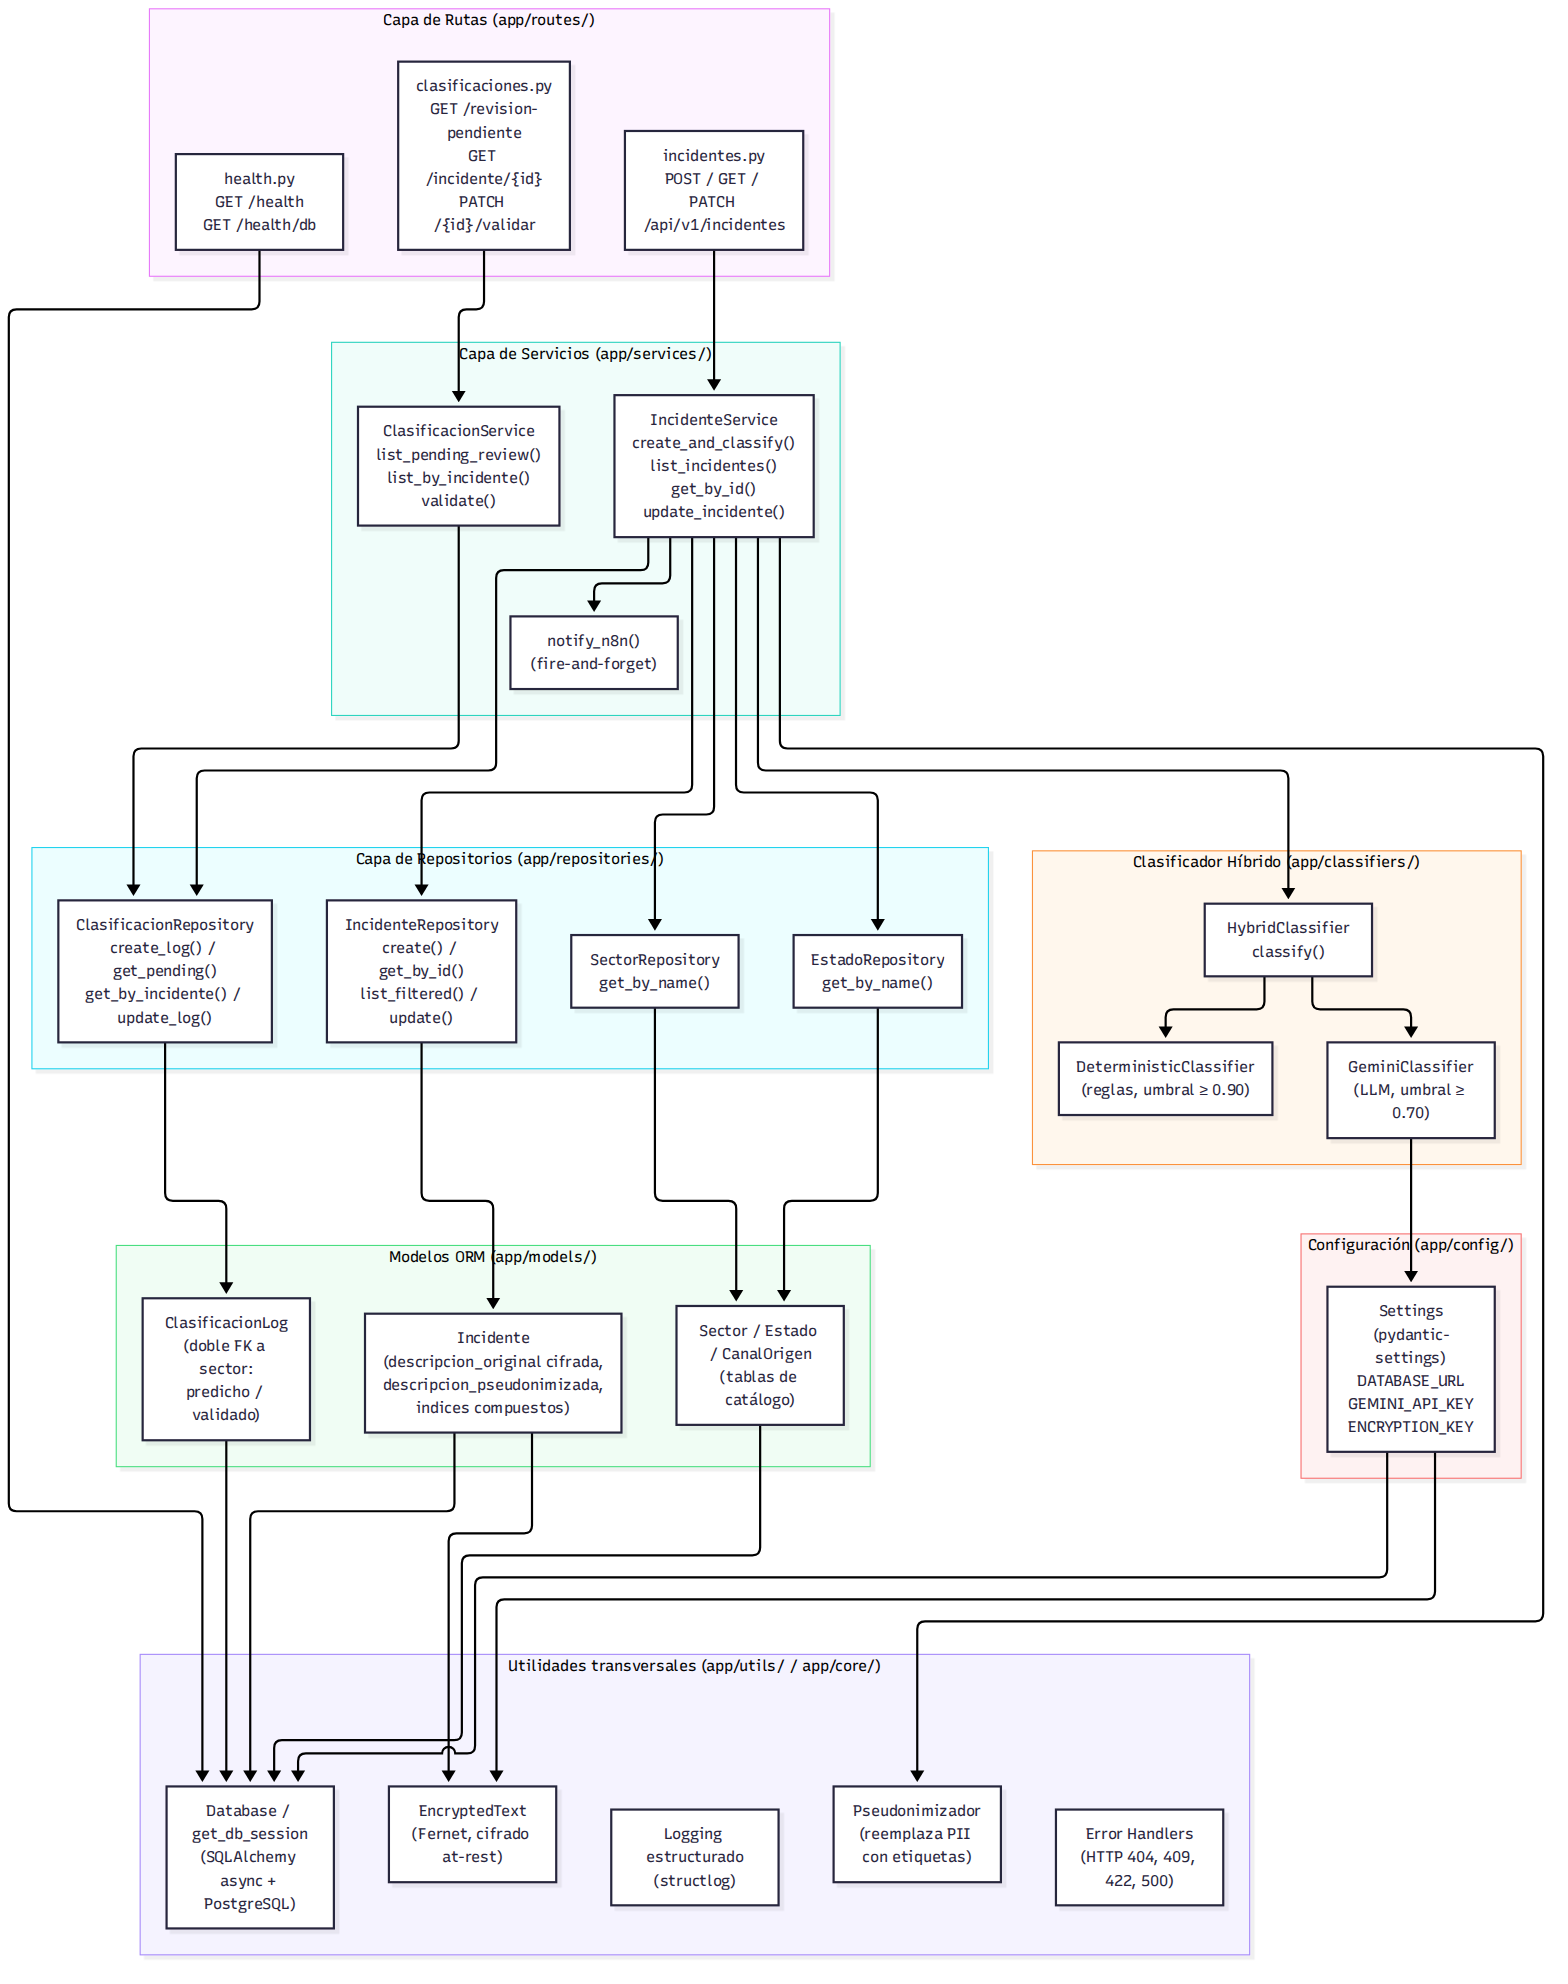
\includegraphics[width=0.80\textwidth,height=0.9\textheight,keepaspectratio]{componentes}
\caption[Diagrama de componentes del módulo Python organizado en capas]{Diagrama de componentes del módulo Python organizado en capas (routes, services, repositories, classifiers). Describe la configuración entregada (release \texttt{v1.2.5}): el filtro determinístico cortocircuita con señal dominante y puntaje de correctitud \(\geq 0{,}5166\) sin derivar por su confianza, la revisión por confianza menor que 0,70 rige solo sobre Gemini, la etapa de reserva deriva siempre, y el disparador por reportante no identificado en el directorio es posterior a la campaña (c-82, 13-10-2026; \autoref{tab:configuracion-evaluada-entregada}). Fuente: \texttt{docs/diagrams/componentes.md}.}
\label{fig:componentes}
\end{figure}

La trazabilidad operativa se garantiza mediante registros estructurados en cada capa, accesibles desde la capa de orquestación. La Figura~\ref{fig:arquitectura} representa esquemáticamente el flujo de información entre capas.

\begin{figure}[htbp]
\centering
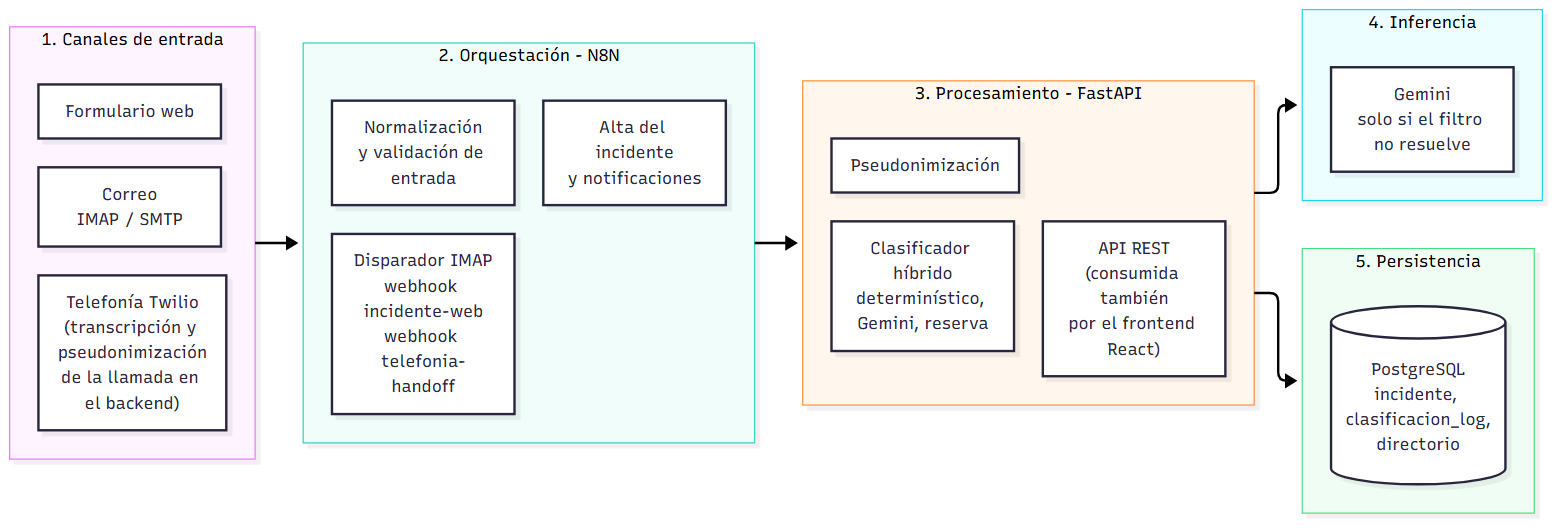
\includegraphics[width=\textwidth]{arquitectura_sistema}
\caption[Diagrama de arquitectura del sistema]{Diagrama de arquitectura del sistema: cinco capas y tres canales de entrada (correo, formulario web y telefonía), en la configuración entregada (release \texttt{v1.2.5}). Fuente versionada: \texttt{docs/diagrams/arquitectura\_sistema.md} (Anexo~\ref{sec:anexo-diagrama-arquitectura}).}
\label{fig:arquitectura}
\end{figure}

\begin{figure}[htbp]
\centering
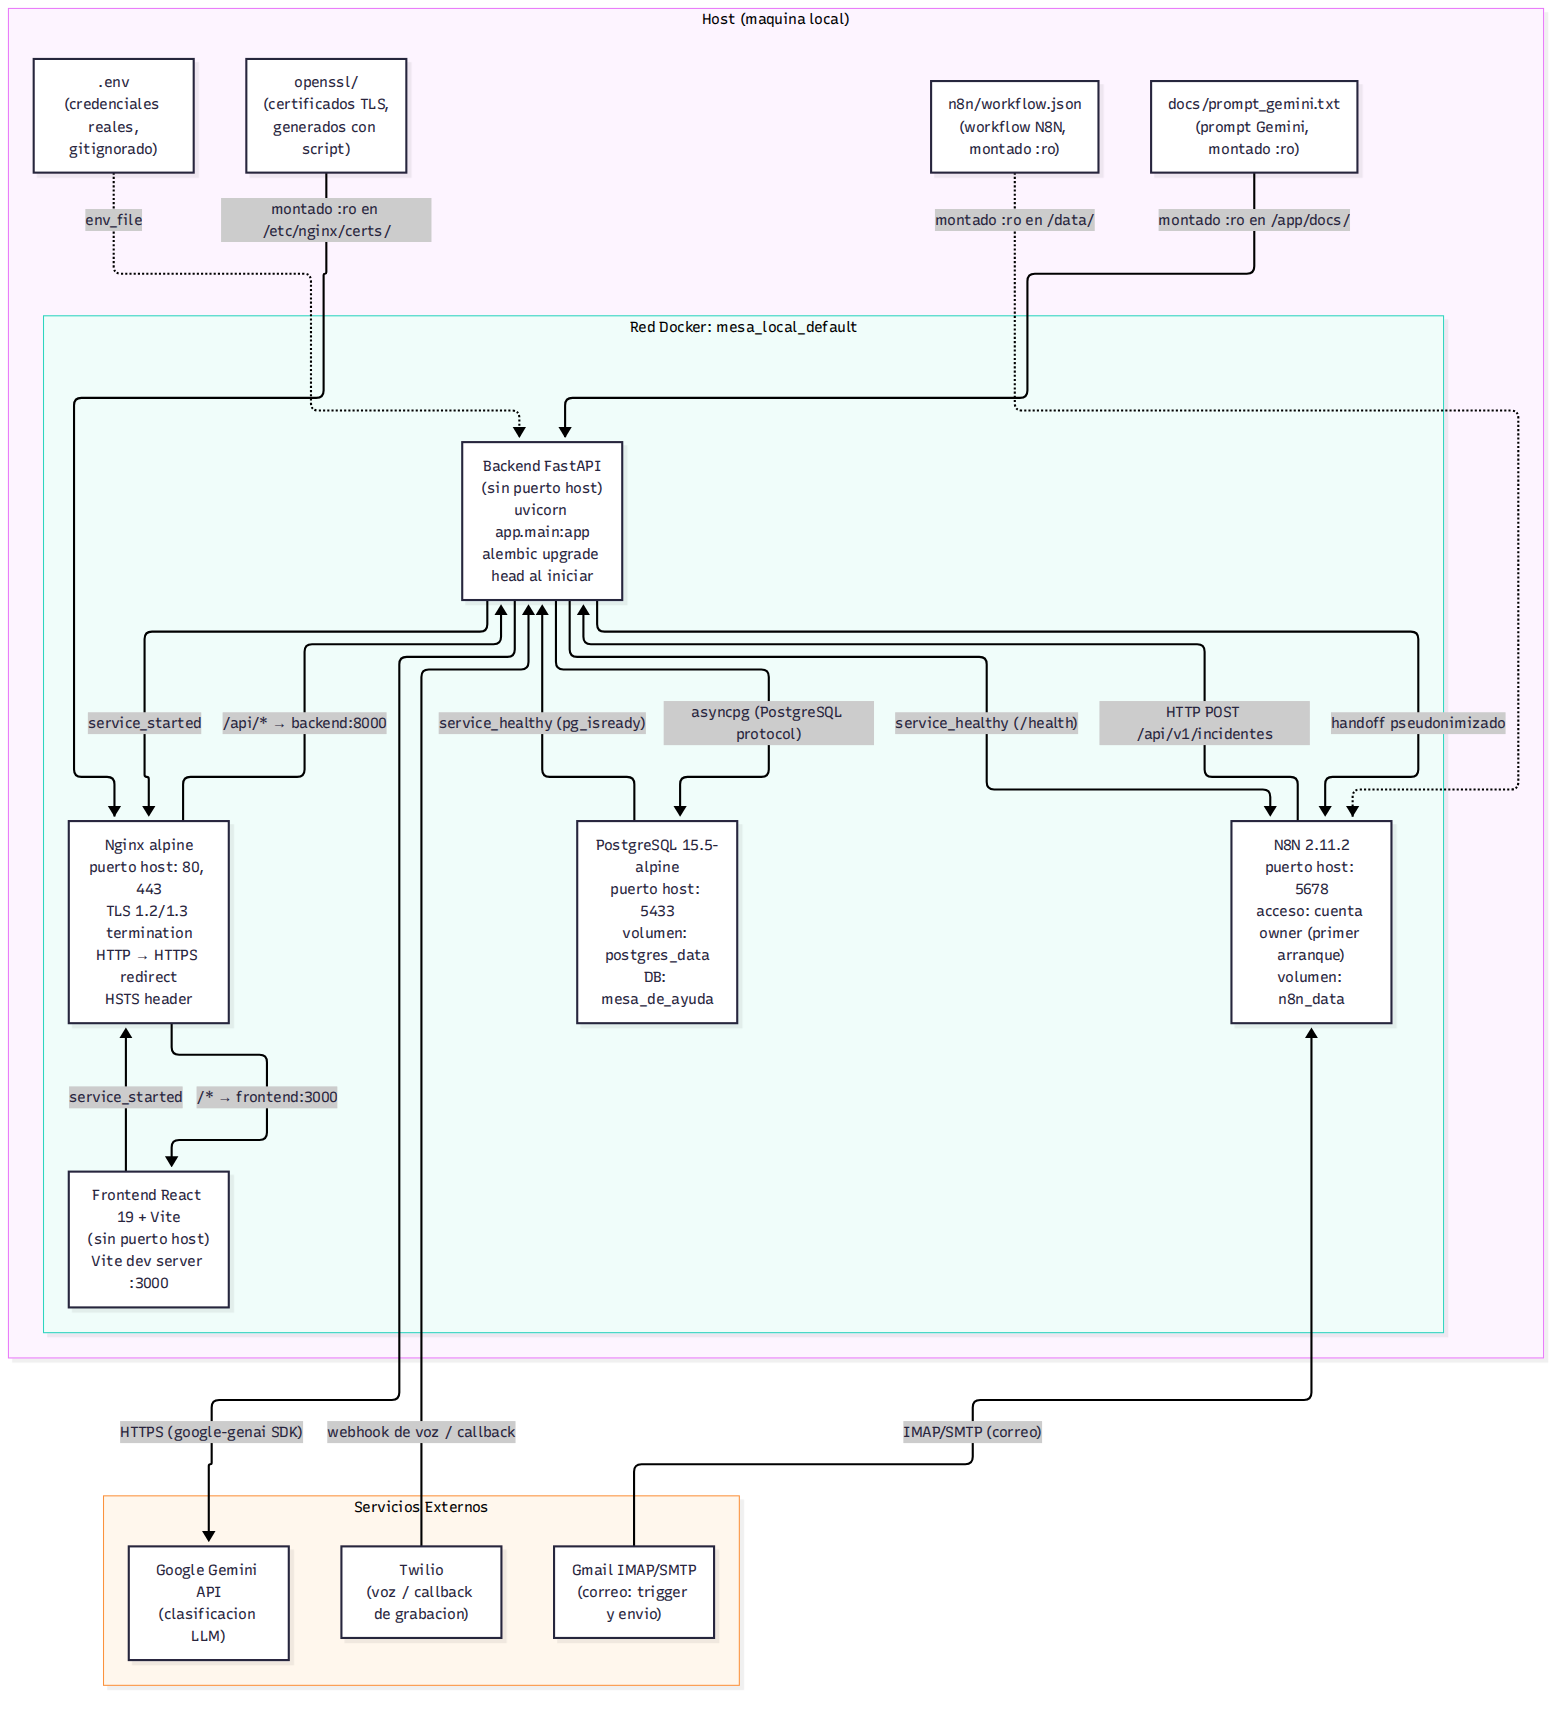
\includegraphics[width=0.92\textwidth]{despliegue}
\caption{Diagrama de despliegue del entorno local. Servicios, red Docker, volúmenes y servicios externos.}
\label{fig:despliegue}
\end{figure}

\begin{figure}[htbp]
\centering
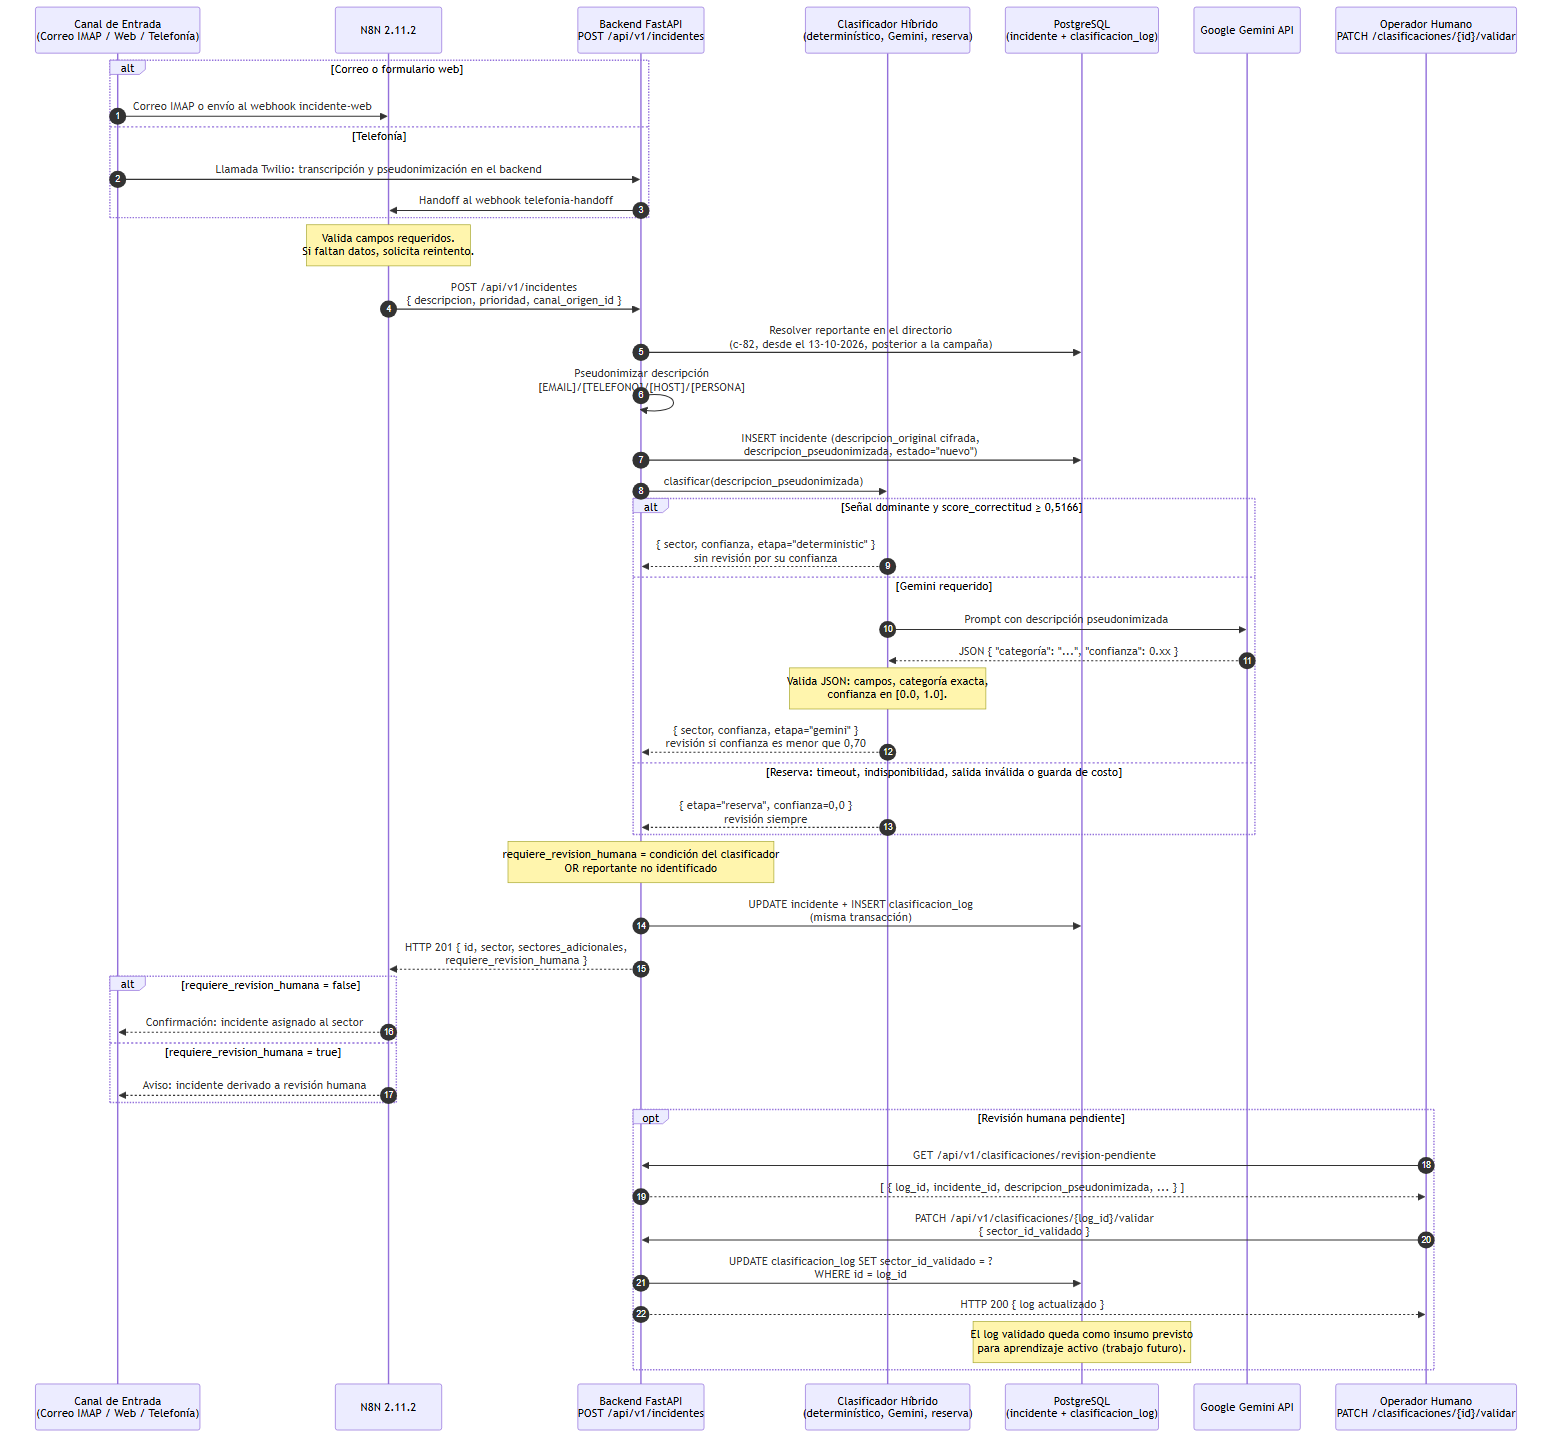
\includegraphics[width=\textwidth]{secuencia}
\caption[Diagrama de secuencia del flujo extremo a extremo de un incidente]{Diagrama de secuencia del flujo extremo a extremo de un incidente, desde el canal de entrada hasta la confirmación o la derivación a revisión humana, en la configuración entregada (release \texttt{v1.2.5}). El disparador por reportante no identificado en el directorio es posterior a la campaña (c-82, 13-10-2026): véase la \autoref{tab:configuracion-evaluada-entregada}.}
\label{fig:secuencia}
\end{figure}

\subsection{Capa de canales de entrada}\label{subsec:capa-canales}

La capa de canales de entrada habilita tres vías paralelas a través de las cuales un usuario puede reportar un incidente. La primera es el correo electrónico, monitoreado mediante IMAP/SMTP que detecta nuevos mensajes en una casilla institucional dedicada. La segunda vía es un formulario web implementado como aplicación React de página única (SPA) que se comunica directamente con la API REST del módulo de procesamiento. La autenticación se realiza mediante tokens JWT (JSON Web Tokens) con usuario y contraseña; la autenticación única corporativa (SSO) se prevé como evolución para entornos productivos (\autoref{sec:recomendaciones}). La tercera vía es la llamada telefónica, en la cual el usuario marca un número virtual provisto por Twilio, recibe instrucciones por voz pregrabadas y deja su solicitud; la grabación es transcrita automáticamente por el servicio de reconocimiento del habla del proveedor y enviada al flujo N8N mediante webhook posterior al cuelgue. El script TwiML que define el flujo de la llamada —incluyendo el mensaje de bienvenida en español rioplatense y la configuración de grabación— se implementa en el módulo de backend del proyecto (\texttt{app/cost\_guard/twiml.py}), versionado en el repositorio. Esta diversidad de canales amplía la accesibilidad del sistema y reduce las barreras al reporte oportuno.

\subsection{Capa de orquestación}\label{subsec:capa-orquestacion}

N8N actúa como orquestador principal del flujo de trabajo: recibe la entrada de cada canal, la normaliza en una estructura unificada y coordina la clasificación y la persistencia del incidente. La descripción operativa detallada del flujo ---los disparadores por canal, la estructura normalizada con identificador único (UUID v4), la invocación al módulo Python y la persistencia del ticket--- se desarrolla en la \autoref{subsec:construccion-flujo-n8n}. Los registros de cada ejecución se conservan durante 30 días para fines de auditoría y diagnóstico operativo; constituyen un conjunto de datos distinto de los incidentes, cuya retención se rige por la política declarada en la \autoref{subsec:principios-datos}.

\subsection{Capa de procesamiento}\label{subsec:capa-procesamiento}

El módulo de procesamiento se implementó como un servicio web ligero utilizando el marco FastAPI~0.115, expuesto sobre un servidor ASGI Uvicorn 0.30.6 (versiones de la configuración evaluada; Anexo~B, Tabla~\ref{tab:configuracion-evaluada-entregada}) \parencite{Tiangolo2024_fastapi}. La elección de FastAPI obedece a su soporte nativo de validación de esquemas mediante Pydantic, su rendimiento competitivo y su documentación automática conforme a la especificación OpenAPI~3.1.

Las dependencias del módulo se organizan por capas funcionales claramente delimitadas. La capa de acceso a datos utiliza SQLAlchemy~2.0 como mapeador objeto-relacional (ORM) y asyncpg como driver asincrónico para PostgreSQL, en coherencia con la operación no bloqueante de FastAPI. La capa de procesamiento textual emplea las bibliotecas regex y unicodedata de la biblioteca estándar de Python para normalización ortográfica y eliminación de signos diacríticos. La capa de inferencia se comunica con la interfaz oficial del modelo \texttt{gemini-3.6-flash} mediante el cliente google-genai >=2.20.0 de la configuración evaluada (SDK unificado de Google Generative AI), con los siguientes parámetros de configuración: temperatura \(= 0{,}3\), top\_p \(= 0{,}9\), max\_tokens \(= 100\) y timeout \(= 30\)~s por intento del backend al modelo, con un presupuesto total de \(60\)~s por clasificación. Estos valores corresponden a la configuración adoptada para el despliegue y no a un procedimiento de optimización documentado; su calibración sistemática frente a valores alternativos se plantea como trabajo futuro (\autoref{sec:recomendaciones}). Las bibliotecas NumPy~2.1 y Pandas~2.2 se utilizan exclusivamente para la generación de reportes agregados de desempeño y no participan del flujo de procesamiento individual de incidentes.

\subsection{Subsistema de clasificación híbrido}\label{subsec:subsistema-clasificacion}

El subsistema de clasificación adopta un enfoque híbrido en dos etapas, característica que lo diferencia de aproximaciones puramente basadas en modelo externo. La primera etapa aplica un filtro determinístico basado en expresiones regulares y diccionarios de términos del dominio. La procedencia de los datos empleados para construir el filtro determinístico, redactar las reglas de frontera del prompt y fijar el punto de operación se declara en la \autoref{subsec:interpretacion-resultados}. La especificación detallada del prompt y de los parámetros de configuración del modelo se documenta en el Anexo~H.

Este filtro resuelve de inmediato los incidentes con marcadores léxicos inequívocos y emite dos magnitudes en \([0;1]\) que no son probabilidades de acierto: la \emph{confianza}, índice de fuerza de señal ---margen del sector ganador sobre el segundo, ponderado por la cantidad de patrones coincidentes--- que vale 0 con menos de dos patrones, y el \emph{puntaje de correctitud} (\texttt{score\_correctitud}), que ordena la correctitud esperada. El filtro decide sin consultar al modelo (cortocircuito) cuando la señal es dominante ---sin empate ni ausencia de coincidencias--- y el puntaje alcanza el punto de operación 0,5166; la confianza no interviene y esos casos no se derivan a revisión por su confianza. El punto se derivó por validación cruzada de cinco pliegues sobre el corpus, maximizando la cobertura sin que la precisión del filtro fuera inferior a la del modelo sobre el conjunto que resuelve (0,7385 frente a 0,6769 sobre los 130 casos con predicción de ambas etapas, ambas estimadas dentro de la muestra; \autoref{subsec:sensibilidad-ajustes}), y equivale a resolver los 131 casos con señal dominante.

La segunda etapa, activada únicamente cuando el filtro determinístico no resuelve el caso, consulta al modelo Gemini~3.6 Flash mediante un prompt estructurado en español que incluye una breve descripción de cada categoría, ejemplos representativos balanceados y la solicitud explícita de devolver la categoría asignada y un valor numérico de confianza entre 0 y 1 en formato JSON estricto. El diseño compositivo reserva la capacidad semántica del modelo para los casos que el filtro no resuelve, lo que reduce la latencia y el costo de inferencia. El pipeline completo comprende tres etapas, aplicadas en orden: (1)~el filtro determinístico, (2)~el modelo Gemini y (3)~una etapa de reserva (\emph{fallback}) que, cuando el modelo no responde o no produce una salida válida, fija la confianza en 0,0 y marca siempre el caso para revisión humana. La regla \texttt{requiere\_revision\_humana = (confianza < 0{,}70)} se evalúa solo sobre la salida de la etapa Gemini; la etapa de reserva deriva siempre a revisión, con confianza 0,0, y la etapa determinística no deriva por su confianza. Desde el 13 de octubre de 2026, posterior a las corridas de la campaña, el backend deriva además a revisión el incidente cuyo reportante no se identifica en el directorio de empleados, condición independiente de la clasificación. El desglose de casos resueltos por cada etapa del pipeline sobre el corpus de validación se reporta en la \autoref{sec:resultados}.

El camino de clasificación es único para los tres canales de entrada. Tanto el correo electrónico y el formulario web como la llamada telefónica resuelven su sector mediante esta misma cascada híbrida, aplicada sobre la descripción pseudonimizada del incidente: ningún canal aporta una clasificación precalculada que omita la cascada, de modo que las reglas determinísticas, el prompt y las reglas de frontera se ajustan una sola vez para todo el sistema. El prompt único incorpora reglas de desambiguación de frontera entre sectores adyacentes (acceder o iniciar sesión en una aplicación se orienta a Soporte Tecnico Software; la digitalización, el escáner o la impresora se orientan a Soporte Tecnico Hardware; el servidor, la red, SMTP o una VM se orientan a Sistemas). Desde el punto de vista del costo, la clasificación telefónica dejó de computarse sobre una invocación incondicional al modelo externo: el canal atraviesa el filtro determinístico y solo escala al modelo semántico cuando la cascada lo requiere.

\subsection{Modelo de datos}\label{subsec:modelo-datos}

La persistencia se realiza sobre PostgreSQL~15.5, desplegado en contenedor Docker bajo configuración de respaldo diario y replicación física opcional para entornos productivos \parencite{PostgreSQL2024_docs}. El modelo de datos se organiza alrededor de siete entidades principales, descritas en la Tabla~\ref{tab:entidades}.

\begin{table}[htbp]
\centering
\caption[Entidades principales del modelo de datos]{Entidades principales del modelo de datos de la configuración entregada (release \texttt{v1.2.5}); el atributo \texttt{reportante\_empleado\_id}, el cuarto rol del directorio y el cifrado del contacto son posteriores a la campaña de medición (c-82, c-86 y c-153).}
\label{tab:entidades}
\footnotesize\singlespacing
\begin{tabular}{@{}>{\raggedright\arraybackslash}p{3.4cm} >{\raggedright\arraybackslash}p{5.3cm} >{\raggedright\arraybackslash}p{6.9cm}@{}}
\toprule
\textbf{Tabla} & \textbf{Atributos clave} & \textbf{Descripción} \\
\midrule
\texttt{incidente} & id (PK), descripcion\_original (cifrada), descripcion\_pseudonimizada, prioridad, sector\_id (FK), estado\_id (FK), canal\_origen\_id (FK), reportante\_empleado\_id (FK), requiere\_revision\_humana & Tabla central: descripción original cifrada en reposo y descripción pseudonimizada, prioridad, sector asignado, estado actual, canal de origen, reportante resuelto en el directorio e indicador de revisión humana. \\
\texttt{sector} & id (PK), nombre & Catálogo de los cinco sectores canónicos: Seguridad Informatica, Soporte Tecnico Hardware, Soporte Tecnico Software, Bases de Datos y Sistemas. \\
\texttt{estado} & id (PK), nombre, es\_terminal & Catálogo de estados: nuevo, en proceso, en espera, resuelto y cerrado. \\
\texttt{canal\_origen} & id (PK), nombre & Catálogo de canales: correo, formulario web y llamada telefónica. \\
\texttt{clasificacion\_log} & id (PK), incidente\_id (FK), sector\_id\_predicho (FK), sector\_id\_validado (FK), confianza, etapa, requiere\_revision\_humana & Registro de cada decisión del clasificador, con el sector predicho, la confianza asociada, la etapa que resolvió, el indicador de revisión y el sector validado por el sector responsable. \\
\texttt{users} & id (PK), username (UNIQUE), hashed\_password, is\_active & Almacena credenciales de operadores para autenticación JWT. \\
\texttt{directorio\_empleado} & id (PK), legajo (UNIQUE), nombre, email y telefono (cifrados), email\_bidx (UNIQUE), telefono\_bidx, sector\_id (FK), rol, activo, fecha\_baja, user\_id (FK) & Directorio institucional de empleados para resolución de contacto y notificación. El correo y el teléfono se cifran en reposo con Fernet y se buscan mediante un índice ciego (HMAC-SHA-256), según la decisión de c-153; el campo \texttt{rol} admite cuatro valores: usuario final, mesa de ayuda, administrador del directorio y gestión de incidentes. La columna \texttt{fecha\_baja} registra la desactivación y sostiene la retención (relación laboral activa más un año). \\
\bottomrule
\end{tabular}
\par\smallskip
{\footnotesize\textit{Fuente:} elaboración propia a partir de \texttt{App/Backend/app/models/}.\par}
\end{table}

El canal de origen constituye una entrada opcional del backend: el esquema de creación de incidentes acepta \texttt{canal\_origen\_id} como campo anulable, de modo que un incidente puede registrarse sin canal conocido. La entidad central \texttt{incidente} referencia mediante claves foráneas a los catálogos de sector, estado y canal de origen, y mantiene una relación uno a muchos con \texttt{clasificacion\_log} para preservar la trazabilidad histórica de las decisiones del clasificador. El número de incidente que se comunica al usuario corresponde al identificador único del registro, formateado para su legibilidad; la incorporación de un prefijo configurable se prevé como evolución futura (\autoref{sec:recomendaciones}). El esquema completo, incluyendo restricciones de integridad referencial e índices secundarios, se documenta en el Anexo~C. El directorio de empleados (\texttt{directorio\_empleado}) se vincula opcionalmente con la tabla de autenticación mediante \texttt{user\_id} y referencia el catálogo de sectores mediante \texttt{sector\_id}; su campo \texttt{rol} distingue al usuario final, a la mesa de ayuda, al administrador del directorio y a la gestión de incidentes (cuatro valores; \autoref{tab:entidades}).

\begin{figure}[htbp]
\centering
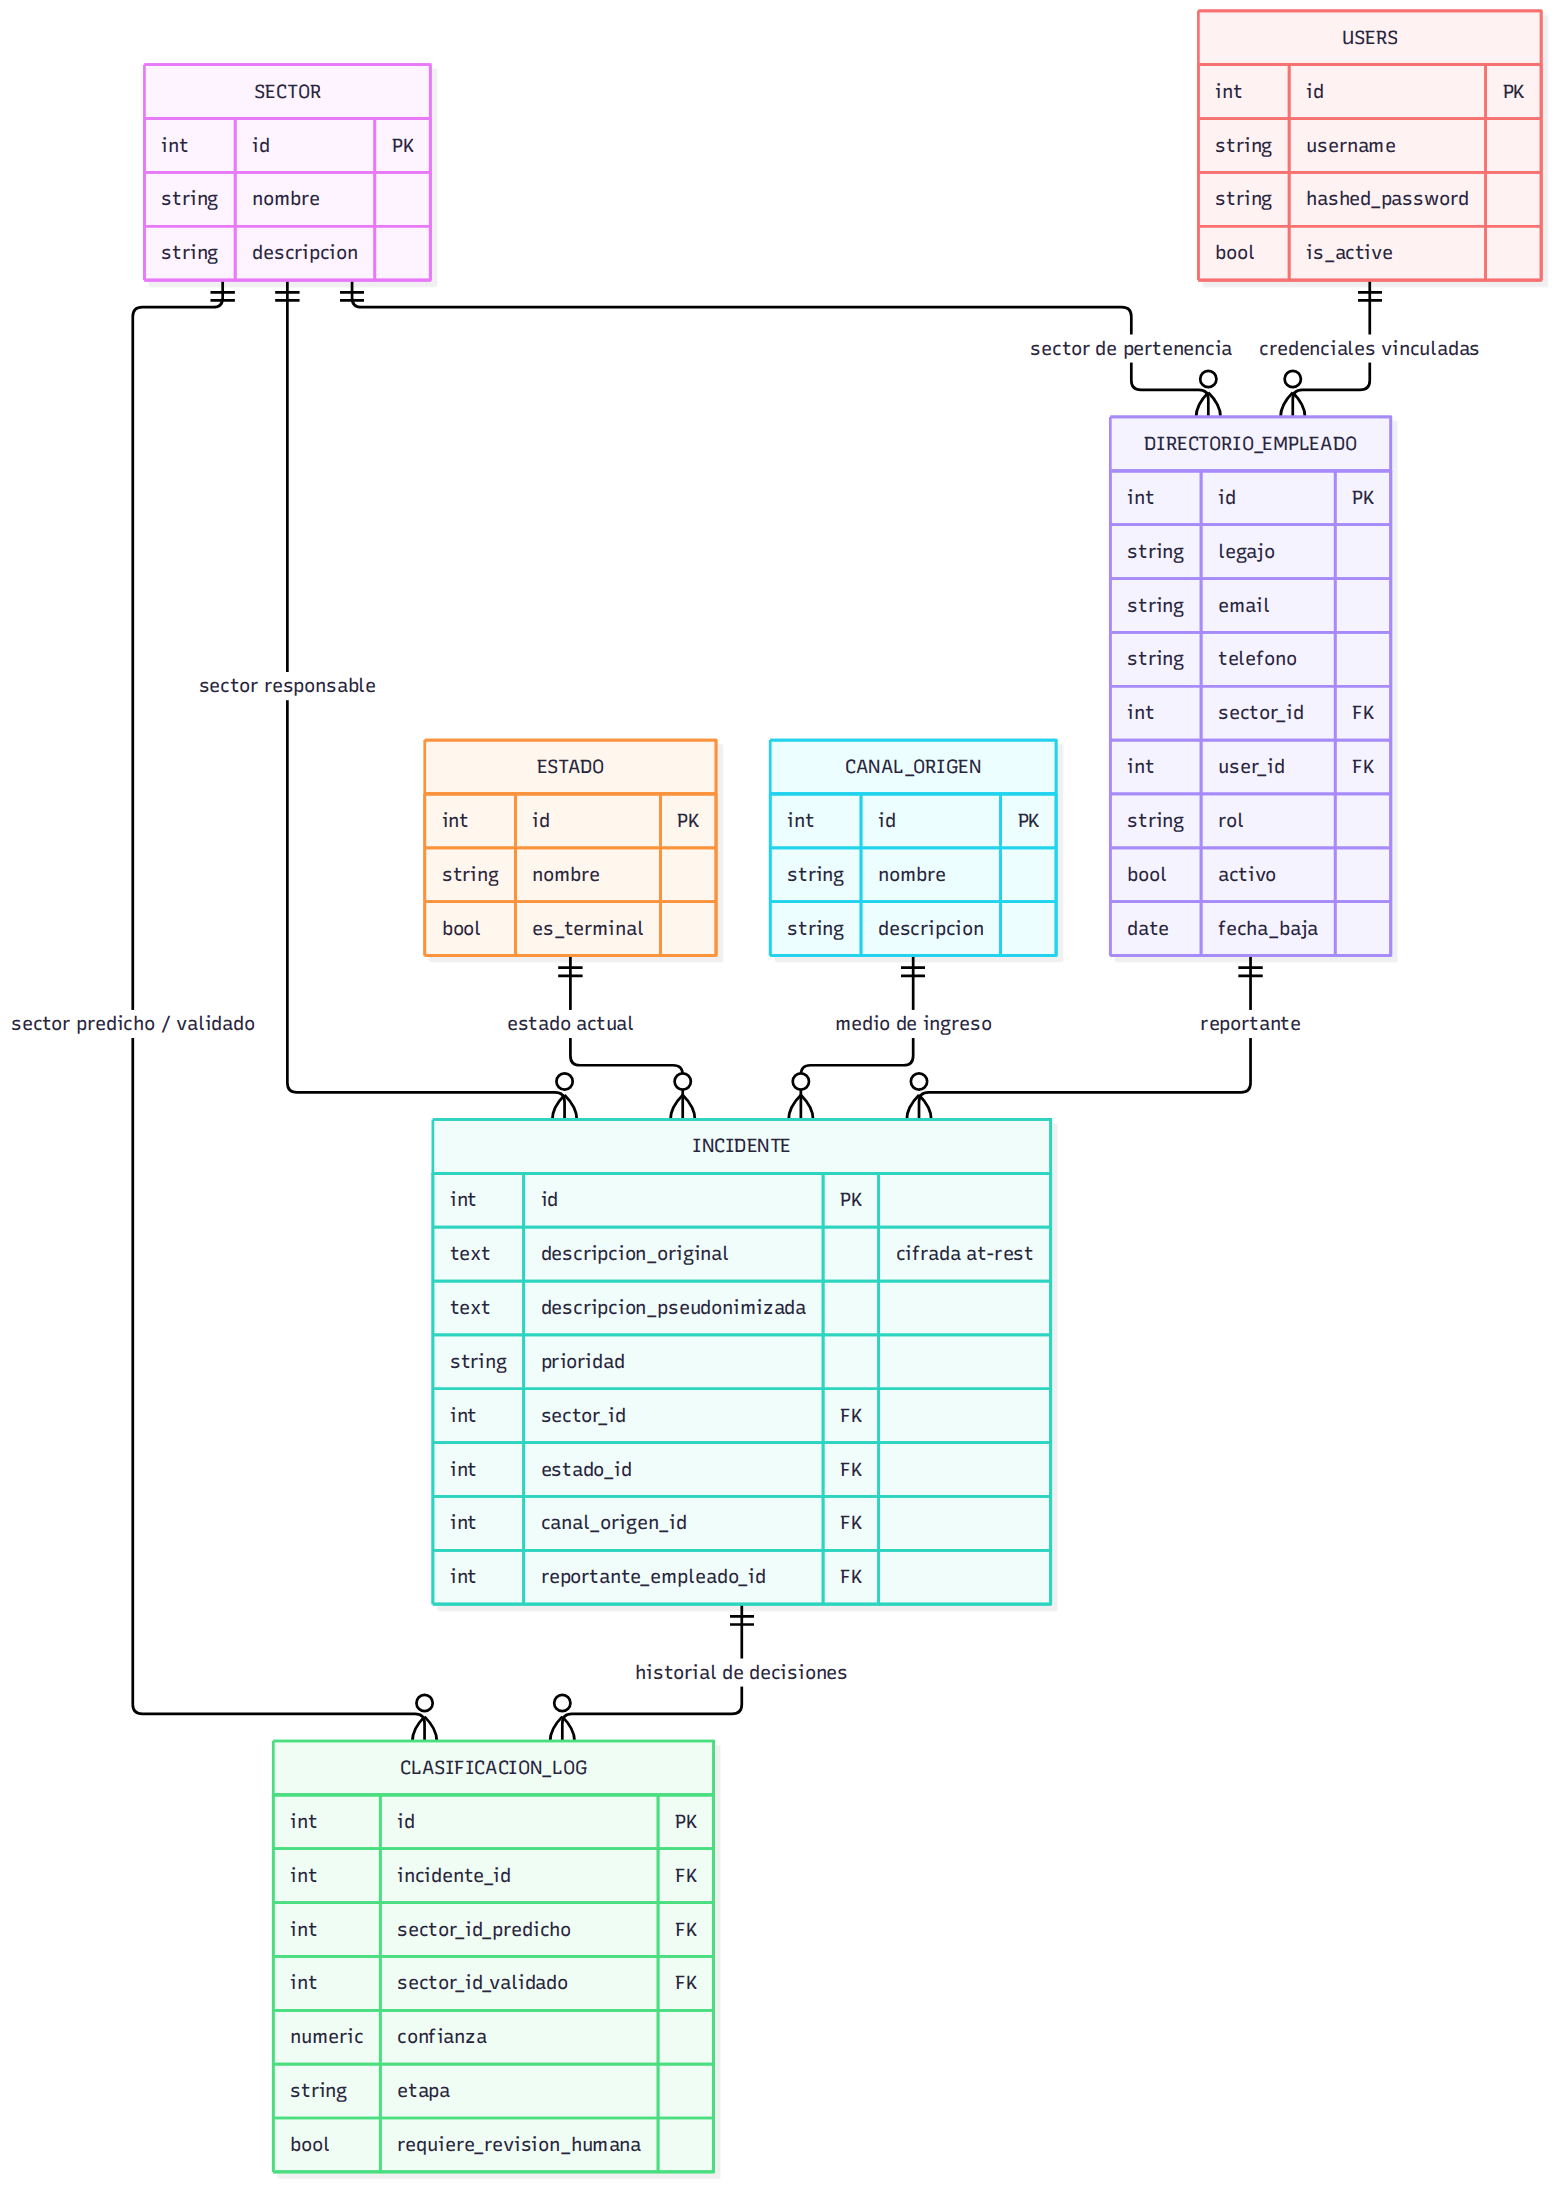
\includegraphics[width=0.85\textwidth]{er_modelo_datos}
\caption[Diagrama entidad-relación de las siete entidades principales]{Diagrama entidad-relación de las siete entidades principales del modelo de datos de la configuración entregada (release \texttt{v1.2.5}; esquema completo en el Anexo~C).}
\label{fig:er_modelo_datos}
\end{figure}

\subsection{Contrato de la interfaz REST}\label{subsec:contrato-rest}

La interfaz de programación de aplicaciones expuesta por el módulo Python sigue el estilo arquitectónico REST \parencite{Fielding2002_rest}, con representación de recursos mediante identificadores uniformes, uso semántico de los métodos HTTP estándar y comunicación sin estado del lado del servidor. La autenticación se realiza mediante tokens JWT (JSON Web Tokens) firmados con HS256, validados en cada solicitud mediante el esquema OAuth2PasswordBearer de FastAPI. La Tabla~\ref{tab:api} sintetiza los principales puntos de entrada.

\begin{table}[htbp]
\centering
\caption{Puntos de entrada principales de la interfaz REST}
\label{tab:api}
\small
\begin{tabular}{@{}p{1.8cm} >{\raggedright\arraybackslash}p{5.2cm} p{1.8cm} >{\raggedright\arraybackslash}p{4.8cm}@{}}
\toprule
\textbf{Método} & \textbf{Ruta} & \textbf{Código} & \textbf{Función} \\
\midrule
\multicolumn{4}{@{}l}{\textbf{Autenticación}} \\
POST & \texttt{/api/v1/auth/login}, \texttt{/refresh}, \texttt{/logout} & 200 OK & Inicio y renovación de sesión y cierre de sesión de operadores. \\
GET & \texttt{/api/v1/auth/me} & 200 OK & Recupera el perfil del operador autenticado. \\
\midrule
\multicolumn{4}{@{}l}{\textbf{Incidentes}} \\
POST & \texttt{/api/v1/incidentes} & 201 Created & Crea un nuevo ticket y devuelve el identificador generado. \\
GET & \texttt{/api/v1/incidentes/\{id\}} & 200 OK & Recupera la información de un ticket por su identificador. \\
PATCH & \texttt{/api/v1/incidentes/\{id\}} & 200 OK & Actualiza los campos editables de un ticket. \\
\midrule
\multicolumn{4}{@{}l}{\textbf{Clasificaciones}} \\
GET & \texttt{/api/v1/clasificaciones/incidente/\{id\}} & 200 OK & Recupera la trazabilidad de la clasificación de un incidente. \\
GET & \texttt{/api/v1/clasificaciones/revision-pendiente} & 200 OK & Lista los casos derivados a revisión humana. \\
PATCH & \texttt{/api/v1/clasificaciones/\{log\_id\}/validar} & 200 OK & Registra la categoría validada por el sector responsable. \\
\midrule
\multicolumn{4}{@{}l}{\textbf{Estadísticas}} \\
GET & \texttt{/api/v1/estadisticas/resumen}, \texttt{/tendencias} & 200 OK & Agregados y series temporales para el dashboard. \\
\midrule
\multicolumn{4}{@{}l}{\textbf{Salud}} \\
GET & \texttt{/health} y \texttt{/health/db} & 200 OK & Verificación de salud del servicio para monitoreo externo. \\
\bottomrule
\end{tabular}
\par\smallskip
{\footnotesize\textit{Fuente:} elaboración propia.\par}
\end{table}

Los códigos de estado HTTP se utilizan conforme a su semántica original: 201 cuando un recurso se crea exitosamente, 200 cuando una consulta se atiende con éxito, 400 cuando los datos de entrada no validan el esquema esperado, 401 cuando la autenticación falla, y 500 cuando ocurre un error interno no recuperable. La Tabla~\ref{tab:api} no es exhaustiva: reúne los grupos principales de puntos de entrada, mientras que el contrato completo de la interfaz ---que comprende la totalidad de las rutas expuestas--- se documenta en el Anexo~D y se versiona en \texttt{docs/openapi.json}; la especificación OpenAPI~3.1 la genera FastAPI automáticamente.

\newpage


% --- Capitulo 6: Implementacion ---
%==============================================================================
% Capítulo 6: Implementación
%==============================================================================
\section{Implementación}\label{sec:implementacion}

\subsection{Entorno de despliegue y dependencias}\label{subsec:entorno-despliegue}

La implementación del sistema se llevó a cabo combinando componentes de código abierto ---Python, FastAPI y PostgreSQL--- con N8N, cuya licencia Sustainable Use (\emph{fair-code}) permite auditar su código fuente, con el objetivo de garantizar la portabilidad, la reproducibilidad y la auditoría de seguridad de la solución en organizaciones medianas. Toda la infraestructura se encapsula mediante contenedores Docker, orquestados localmente por Docker Compose para los entornos de desarrollo y preproducción; la migración a un cluster Kubernetes~1.30 para el entorno productivo se plantea como trabajo futuro y no cuenta con manifiestos de despliegue en esta versión (\autoref{sec:recomendaciones}).

Las versiones específicas de los componentes son: N8N~2.11.2, Python~3.12, PostgreSQL~15.5 con volumen persistente, FastAPI~0.115, Uvicorn 0.30.6, SQLAlchemy~2.0, y el cliente google-genai >=2.20.0 (SDK unificado de Google Generative AI) para la comunicación con el modelo \texttt{gemini-3.6-flash}. Todos los servicios se despliegan sobre imágenes Docker oficiales (\texttt{python:3.12-slim} y \texttt{postgres:15.5-alpine}). La gestión de dependencias del módulo Python se realiza mediante un archivo \texttt{requirements.txt} con versiones fijadas (\emph{pinned}) para garantizar la reproducibilidad de las compilaciones en distintos entornos.

\subsection{Construcción del módulo Python}\label{subsec:construccion-modulo-python}

La selección del marco de trabajo para el servicio de procesamiento implicó la evaluación de tres alternativas: Flask, Django REST Framework y FastAPI. Flask, ampliamente adoptado en el ecosistema Python por su simplicidad, carece de validación nativa de esquemas y de generación automática de documentación OpenAPI, funcionalidades que el proyecto requería para garantizar la calidad de la interfaz REST. Django REST Framework, por su parte, ofrece un conjunto completo de herramientas para la construcción de interfaces de programación de aplicaciones, pero su modelo de operación sincrónico y la inclusión de componentes no requeridos por el proyecto ---tales como el ORM de Django y el motor de plantillas--- incrementaban la complejidad de la base de código sin aportar beneficios funcionales para una arquitectura de microservicio acotado. FastAPI~0.115, sustentado sobre el servidor ASGI Uvicorn 0.30.6, ofrece tres ventajas determinantes para el proyecto: validación automática de esquemas de entrada y salida mediante Pydantic~v2, generación de documentación interactiva conforme a la especificación OpenAPI~3.1 sin configuración adicional, y operación asincrónica nativa que permite manejar las llamadas concurrentes desde N8N sin bloquear el hilo de ejecución principal \parencite{Tiangolo2024_fastapi}. La madurez del ecosistema de FastAPI, su adopción creciente en la industria y la disponibilidad de documentación exhaustiva en español consolidaron la decisión.

El módulo Python expone su contrato REST organizado en capas, según la estructura descrita en la \autoref{sec:arquitectura}, con una separación clara entre responsabilidades:

\begin{itemize}
  \item \textbf{models}: entidades del modelo de dominio mapeadas mediante SQLAlchemy~2.0.
  \item \textbf{schemas}: modelos de validación y serialización con Pydantic~v2.
  \item \textbf{services}: lógica de aplicación (IncidenteService, ClasificacionService).
  \item \textbf{repositories}: acceso a datos, aislando las consultas SQL del resto de la aplicación.
  \item \textbf{classifiers}: lógica del clasificador híbrido (filtro determinístico + LLM).
  \item \textbf{routes}: enrutadores REST que delegan en los servicios correspondientes.
  \item \textbf{core}: configuración de base de datos, manejo de errores y logging estructurado.
\end{itemize}

La construcción se realiza bajo un esquema de inyección de dependencias gestionado por las funcionalidades nativas de FastAPI (\texttt{Depends}), lo que facilita el reemplazo de implementaciones durante la ejecución de pruebas unitarias y de integración. Esta arquitectura permite, por ejemplo, sustituir el clasificador real por una implementación simulada durante las pruebas sin modificar el código de los servicios que lo consumen. La gestión de credenciales se realiza exclusivamente mediante variables de entorno, en línea con el principio de configuración de la metodología Twelve-Factor App \parencite{Wiggins2017_12factor}.

\subsection{Construcción del flujo en N8N}\label{subsec:construccion-flujo-n8n}

El flujo de orquestación implementado en N8N comprende 32 nodos (29 operativos más 3 notas adhesivas), organizados en siete etapas funcionales pero con ramificaciones específicas por canal. La elección de N8N como plataforma de orquestación, frente a alternativas como Apache Airflow, Zapier o Make, obedeció a tres criterios concurrentes. El primero, de naturaleza operativa, radica en que N8N admite despliegue completamente autoalojado bajo Docker, manteniendo los flujos de procesamiento y los datos dentro del perímetro organizacional. Zapier y Make operan exclusivamente como servicios en la nube, lo que las descarta en escenarios donde el procesamiento de datos sensibles exige control de infraestructura. Apache Airflow, aunque autoalojable, diseña sus flujos como grafos acíclicos dirigidos programados por intervalos temporales; ese paradigma resulta adecuado para procesos de extracción, transformación y carga de datos pero forzadamente inadecuado para un sistema reactivo que debe responder en tiempo real a eventos de entrada no programados \parencite{Apache2024_airflow}. El segundo criterio refiere al modelo de construcción visual que N8N ofrece sobre un editor de nodos arrastrables: la curva de aprendizaje de esta interfaz es sustancialmente menor que la de alternativas centradas en definición programática de flujos, lo que permitió al equipo concentrar el esfuerzo en la lógica de negocio antes que en la sintaxis de definición de procesos. El tercer criterio se vincula con la licencia de código fuente disponible (\emph{fair-code}) que habilita la auditoría de seguridad del núcleo de orquestación \parencite{n8n2024_docs}.

La composición de los 29 nodos responde a un patrón de procesamiento por canal, de cinco pasos, que se replica para cada medio de ingreso con ramificaciones específicas según el canal:

\begin{enumerate}[leftmargin=*]
  \item \textbf{Recepción}: Tres disparadores (\emph{triggers}) reciben las entradas desde correo electrónico (IMAP), formulario web (Webhook) y telefonía (trigger de Twilio). La decisión de separar los disparadores por canal, en lugar de unificar la recepción mediante un único webhook con discriminación interna, se fundamenta en la necesidad de preservar la configuración de autenticación y los parámetros de reintento específicos de cada protocolo.
  \item \textbf{Normalización}: Un nodo de transformación (\emph{Function}) homogeniza la estructura del mensaje en un formato unificado \parencite{Hohpe2003_eip} con campos de identificador único (UUID v4), marca temporal, canal de origen, remitente y descripción textual normalizada. Esta etapa elimina las diferencias de formato entre canales y garantiza que las capas posteriores procesen siempre la misma estructura de datos, independientemente de la vía de entrada.
  \item \textbf{Clasificación y persistencia}: Un nodo HTTP invoca el endpoint \texttt{POST /api/v1/incidentes} del módulo Python enviando la descripción textual junto con los metadatos del canal. La clasificación no se expone como punto de entrada independiente sino que se encuentra embebida dentro de la creación del incidente: el clasificador híbrido se invoca internamente durante la creación, que persiste el ticket en la misma operación, y la respuesta incluye el identificador del ticket, la categoría asignada y el indicador de revisión humana (\texttt{requiere\_revision\_humana}), que el backend activa según las condiciones descritas en la etapa de evaluación. El canal telefónico no constituye una excepción: su clasificación se resuelve dentro del backend mediante la misma cascada híbrida que los canales escritos, aplicada sobre la descripción pseudonimizada, y el cuerpo de la creación no transporta una clasificación precalculada.
  \item \textbf{Evaluación}: Aguas abajo del POST, un nodo condicional (\emph{IF}) evalúa el indicador de revisión humana devuelto por el backend. Cuando el indicador está activo el flujo notifica al operador designado por correo electrónico y registra el evento en la auditoría; cuando no lo está, el flujo continúa automáticamente con las confirmaciones al usuario. Con anterioridad al POST, un nodo de validación de entrada verifica que la descripción no esté vacía y respete la longitud mínima y máxima aceptada por el backend, de modo que una entrada inválida no genera un incidente. El backend activa el indicador cuando la etapa Gemini devuelve una confianza inferior a 0,70, cuando interviene la etapa de reserva o cuando el reportante no se identifica en el directorio de empleados; los casos que resuelve el filtro determinístico no se derivan por su confianza (\autoref{subsec:subsistema-clasificacion}). La calibración de la confianza del modelo se analiza en la Sección~\ref{subsec:calibracion}.
  \item \textbf{Notificación}: Tres nodos posteriores notifican al usuario por el canal correspondiente y registran la ejecución en el sistema de auditoría; la persistencia del ticket ocurre en el mismo POST de creación, que almacena el incidente y su clasificación en una sola operación. El paralelismo de la notificación garantiza que la demora de un canal (por ejemplo, el envío de correo electrónico) no bloquee el registro de auditoría ni la confirmación por otros medios.
\end{enumerate}

El canal telefónico incorpora un nodo adicional de normalización y validación que prepara la transcripción pseudonimizada antes de incorporarla al flujo principal, pero no determina el sector persistido: la rama de clasificación por agente LLM basada en LangChain fue retirada (decisión OQ1 = A del change c-72). La clasificación del incidente telefónico se rige por el diseño unificado descrito en la \autoref{subsec:subsistema-clasificacion}.

La trazabilidad completa de cada ejecución se preserva almacenando los identificadores de nodo, las marcas temporales de entrada y salida de cada etapa, y los datos de entrada y salida de cada paso del flujo, generando un historial auditable que resulta especialmente valioso en contextos donde la Ley~25.326 exige demostrar el camino recorrido por los datos personales \parencite{Ley25326_2000}. La exportación completa del flujo en formato JSON se incluye en el Anexo~E.

\subsection{Integración del canal telefónico}\label{subsec:integracion-canal-telefonico}

La integración con Twilio se realizó mediante el producto Programmable Voice, complementado con la transcripción automática nativa. El flujo telefónico opera de la siguiente manera: el usuario marca un número virtual asignado a la organización; un script TwiML reproduce un mensaje de bienvenida en español rioplatense y solicita al usuario describir su problema durante un máximo de 45 segundos; la grabación finaliza cuando el usuario presiona la tecla numeral (\texttt{\#}) o transcurrido el tiempo máximo; la grabación se envía al servicio de transcripción de Twilio; y, una vez transcrito el contenido, Twilio invoca un webhook expuesto por N8N con la transcripción textual. A partir de ese punto, el flujo continúa de manera idéntica a la de los canales escritos.

El tiempo de registro del canal telefónico ---medido, para igualar la base de comparación con el flujo manual, desde el inicio de la llamada hasta la confirmación del número de incidente--- promedió 20,1 segundos sobre los 81 casos del corpus. Ese total comprende la duración de la llamada grabada y la latencia de procesamiento posterior al cuelgue; el corpus registra la suma de ambos tramos, no su descomposición por etapa (transcripción, clasificación y persistencia), de modo que no se publica un desglose de latencias que el repositorio no permite reproducir con tamaño de muestra y procedimiento de medición. La grabación está acotada a un máximo de 45~s, de modo que el tiempo telefónico reportado constituye una cota inferior de la duración real de la llamada.

Unificada la clasificación, el canal telefónico dejó de reservar la superficie de costo asociada a la invocación incondicional del agente en N8N. La clasificación pasa a computarse en la superficie de inferencia del backend y solo cuando la cascada híbrida escala al modelo semántico; los casos resueltos por el filtro determinístico no consumen cuota de Gemini. Este traslado de la superficie de costo corresponde a la decisión OQ2 = A del change c-72 y elimina la reserva telefónica del proveedor invocado desde N8N.

\subsection{Desafíos de integración}\label{subsec:desafios-integracion}

La implementación del sistema enfrentó tres desafíos de integración que merecen documentación explícita por su potencial utilidad en replicaciones futuras.

El primer desafío se presentó en la comunicación asincrónica entre N8N y el servicio de clasificación. El nodo HTTP de N8N invoca el endpoint de clasificación de manera sincrónica y espera la respuesta del servidor antes de continuar el flujo. Esta arquitectura, aunque simple de implementar, introduce un punto de fallo único: si el servicio Python no responde dentro del tiempo de espera configurado en el nodo HTTP, el flujo completo se detiene y el incidente queda sin procesar. Esta limitación se asume como conocida en la versión evaluada: no se implementó un mecanismo de reintento con retroceso exponencial ni una cola de respaldo en el servicio Python que retuviera los mensajes durante ventanas de saturación. La disponibilidad ante fallas transitorias del servicio de clasificación queda, por lo tanto, como trabajo futuro, junto con la definición de una política de reintentos idempotente que preserve la trazabilidad de cada intento.

El segundo desafío surgió de la heterogeneidad de los formatos de entrada. Los correos electrónicos incluyen encabezados, firmas corporativas y reenvíos que contaminan el texto que el clasificador recibe; las llamadas telefónicas transcritas introducen errores de reconocimiento del habla, particularmente en términos técnicos (por ejemplo, \texttt{API} transcrito como \texttt{a p i} o \texttt{apeye}); y los formularios web, aunque proveen texto limpio, llegan con una proporción significativa de campos vacíos o con descripciones de una sola palabra. La respuesta a esta heterogeneidad fue doble. Por un lado, se implementó un preprocesador en el nodo de normalización de N8N que elimina firmas, encabezados de reenvío y líneas de disclaimer mediante expresiones regulares específicas del dominio de correo institucional. Por el otro, se enriqueció el prompt enviado al clasificador con instrucciones explícitas para interpretar términos técnicos frecuentemente mal transcritos, lo que mejoró la robustez de la clasificación sobre transcripciones automáticas respecto de la configuración inicial sin estas instrucciones.

El tercer desafío, de naturaleza operativa, se vincula con la persistencia transaccional de la sesión de clasificación. El sistema debe garantizar que una vez que el clasificador asigna una categoría, el incidente se persiste con esa decisión o, en caso de falla de la base de datos, el estado interno del sistema refleje la inconsistencia y pueda recuperarse. La solución adoptó un enfoque pragmático: N8N invoca la creación del incidente ---que clasifica y persiste en una sola operación del backend--- como paso único del flujo. El nodo HTTP de creación declara un enrutamiento de error (\texttt{continueErrorOutput}): ante una falla de persistencia, la ejecución se desvía hacia la rama de error del flujo en lugar de reintentar automáticamente la operación. La recuperación del incidente exige, por lo tanto, una reejecución manual del flujo o el reproceso del mensaje de origen, situación que se asume como limitación conocida de la versión evaluada y se propone como trabajo futuro junto con una política de reintentos idempotente. La tabla de trazabilidad (\texttt{clasificacion\_log}) fue diseñada para admitir múltiples registros de clasificación por incidente, preservando así el historial de cada intento.

\subsection{Conexión con el proceso Scrumban}\label{subsec:conexion-scrumban}

La construcción del sistema fue organizada bajo el esquema Scrumban descrito en la \autoref{sec:marco-metodologico}, ejecutando iteraciones de duración variable, ubicadas sin fechar por separado en los dos períodos de actividad del repositorio (\autoref{fig:cronograma}, Anexo~A). La vinculación entre cada etapa de construcción y los artefactos de implementación producidos se detalla a continuación:

\begin{enumerate}[label=Etapa \arabic*:, leftmargin=*]
  \item La elicitación de requisitos produjo el diseño preliminar de la arquitectura de cinco capas y la especificación de la interfaz REST, documentadas en la \autoref{sec:arquitectura}.
  \item La construcción del módulo Python entregó el modelo de datos, los repositorios con operaciones CRUD asincrónicas y los servicios de negocio. Al cierre de esta etapa, el módulo Python exponía el endpoint de salud y aceptaba la creación de incidentes mediante \texttt{POST /api/v1/incidentes}, con la cobertura de pruebas unitarias medida por pytest-cov sobre los paquetes de rutas, servicios y repositorios (véase la \autoref{subsec:pruebas-automatizadas}).
  \item La configuración inicial del flujo N8N implementó el canal de correo electrónico como vía prioritaria, estableciendo el patrón de procesamiento por canal que luego se replicaría para los canales restantes. Al finalizar esta etapa, el sistema procesaba incidentes por correo electrónico de extremo a extremo, desde la recepción hasta la notificación.
  \item La integración del canal telefónico y la persistencia incorporó Twilio Programmable Voice, el script TwiML y la configuración del webhook de transcripción. Esta etapa fue la que más expuso los desafíos de heterogeneidad de formatos descritos en la \autoref{subsec:desafios-integracion}, y su resolución consumió aproximadamente el 40~\% del esfuerzo de la etapa.
  \item La validación funcional y el ajuste fino del clasificador se concentraron en la calibración del filtro determinístico y del prompt de Gemini. Los ajustes se realizaron a partir de errores observados en el corpus de validación; no se dispuso de un conjunto independiente de incidentes de preproducción (\autoref{subsec:interpretacion-resultados}).
  \item La validación experimental y la documentación final ejecutaron el protocolo de pruebas descrito en la \autoref{sec:marco-metodologico}, recolectaron las mediciones del corpus completo y produjeron el análisis estadístico presentado en la \autoref{sec:resultados}.
\end{enumerate}

La campaña del flujo manual (junio a agosto de 2026) no es una etapa de construcción; la del flujo automatizado (septiembre a octubre de 2026) corresponde a la validación experimental, con \texttt{gemini-3.6-flash} integrado el 24 de septiembre de 2026.

La trazabilidad entre etapas y artefactos, mediada por el tablero Kanban en Jira, permitió al equipo identificar tempranamente los desvíos respecto del plan y redistribuir el esfuerzo cuando la complejidad de un componente superaba la estimación inicial. La adopción de límites de trabajo en curso (WIP) por columna del tablero evitó la acumulación de tareas a medio terminar, una práctica que resultó particularmente valiosa durante las etapas 4 y 5, donde la interdependencia entre módulos exigía finalizar componentes antes de integrarlos.

\subsection{Pruebas automatizadas}\label{subsec:pruebas-automatizadas}

La estrategia de pruebas se sustentó en la pirámide clásica descrita por \textcite{Crispin2009_agile_testing}. En la base se ubicaron las pruebas unitarias del módulo Python construidas con el marco pytest~8.3. La cobertura de código de aplicación se mide con pytest-cov 5.0.0 sobre los paquetes de rutas, servicios y repositorios, mediante el comando \texttt{pytest --cov=app.routes --cov=app.services --cov=app.repositories --cov-report=term-missing}, cuyo reporte se genera en cada ejecución del pipeline de integración continua; la cifra exacta queda sujeta al reporte vigente y no se fija en el texto para no declarar un valor no reproducible. Estas pruebas cubren los clasificadores (determinístico e híbrido), los servicios de negocio, los esquemas de validación y los repositorios de acceso a datos.

En el nivel intermedio se ejecutaron pruebas de integración en dos variantes complementarias: (a)~pruebas rápidas contra SQLite en memoria para la ejecución durante el desarrollo, utilizando el fixture \texttt{db\_session} con rollback por test; y (b)~pruebas de integración contra una instancia real de PostgreSQL~15.5, que validan comportamientos específicos del motor ---integridad de claves foráneas, eliminación en cascada, restricciones UNIQUE, precisión de tipos \texttt{Numeric(5,4)} y zona horaria en \texttt{TIMESTAMPTZ}, índices compuestos y coexistencia de esquemas--- mediante 16 tests con un mecanismo de omisión automática (\texttt{pytest.skip}) cuando PostgreSQL no está disponible. En el nivel superior no se dispone de pruebas de extremo a extremo que instancien N8N y ejecuten el flujo completo: la integración con la plataforma de orquestación se verifica de forma estructural, mediante pruebas que parsean y validan el archivo \texttt{n8n/workflow.json} (composición de nodos, conexiones y límites de costo) y pruebas de API y de base de datos que ejercitan los endpoints y la persistencia del módulo Python. La ejecución del flujo dentro de una instancia N8N activa queda fuera del alcance de la suite automatizada.

El frontend se desarrolló como una aplicación React 19 de página única (SPA) con TypeScript y Vite como herramienta de construcción. La aplicación consta de dos vistas principales: un portal de reporte de incidentes con validación de formularios, y un panel de administración que incluye listado de tickets con filtros combinados, cola de revisión humana para los casos derivados por el backend, y visualización detallada de cada incidente con trazabilidad completa de la decisión del clasificador. La comunicación con el backend se realiza mediante Axios, y la gestión del estado del servidor se apoya en React Query para caching y revalidación automática.

El frontend cuenta con una suite de 357 pruebas automatizadas distribuidas en 56 archivos, construidas con Vitest y Testing Library, que alcanza una cobertura de sentencias del 99,6~\% sobre los paquetes medidos, conforme al reporte reproducido con \texttt{npm run test:coverage}; la cifra queda sujeta al reporte vigente en cada ejecución del pipeline de integración continua.

La integración continua (CI) se ejecuta automáticamente en cada solicitud de incorporación (\emph{pull request}) al repositorio mediante GitHub Actions, ejecutando la suite completa de pruebas unitarias y de integración antes de permitir la fusión a la rama principal. El pipeline de CI incluye verificación de estilo de código (Ruff), ejecución de pruebas con reporte de cobertura, y verificación de sincronización de la especificación OpenAPI.

\subsection{Dashboard de analítica}\label{subsec:dashboard-analitica}

El panel de administración incluye un dashboard de analítica desarrollado con la biblioteca ReCharts de React. Este módulo proporciona visualización agregada de los datos históricos de incidentes, permitiendo identificar tendencias temporales, patrones de fallas recurrentes y desequilibrios en la distribución de carga entre sectores. Esta capacidad de análisis retrospectivo transforma los datos operativos acumulados en inteligencia organizacional accionable. La Figura~\ref{fig:panel_admin} muestra el panel de administración sobre el que se integra esta capacidad analítica, con el listado de tickets, los filtros combinados y la pestaña de revisión humana para los casos derivados por el backend.

\begin{figure}[htbp]
\centering
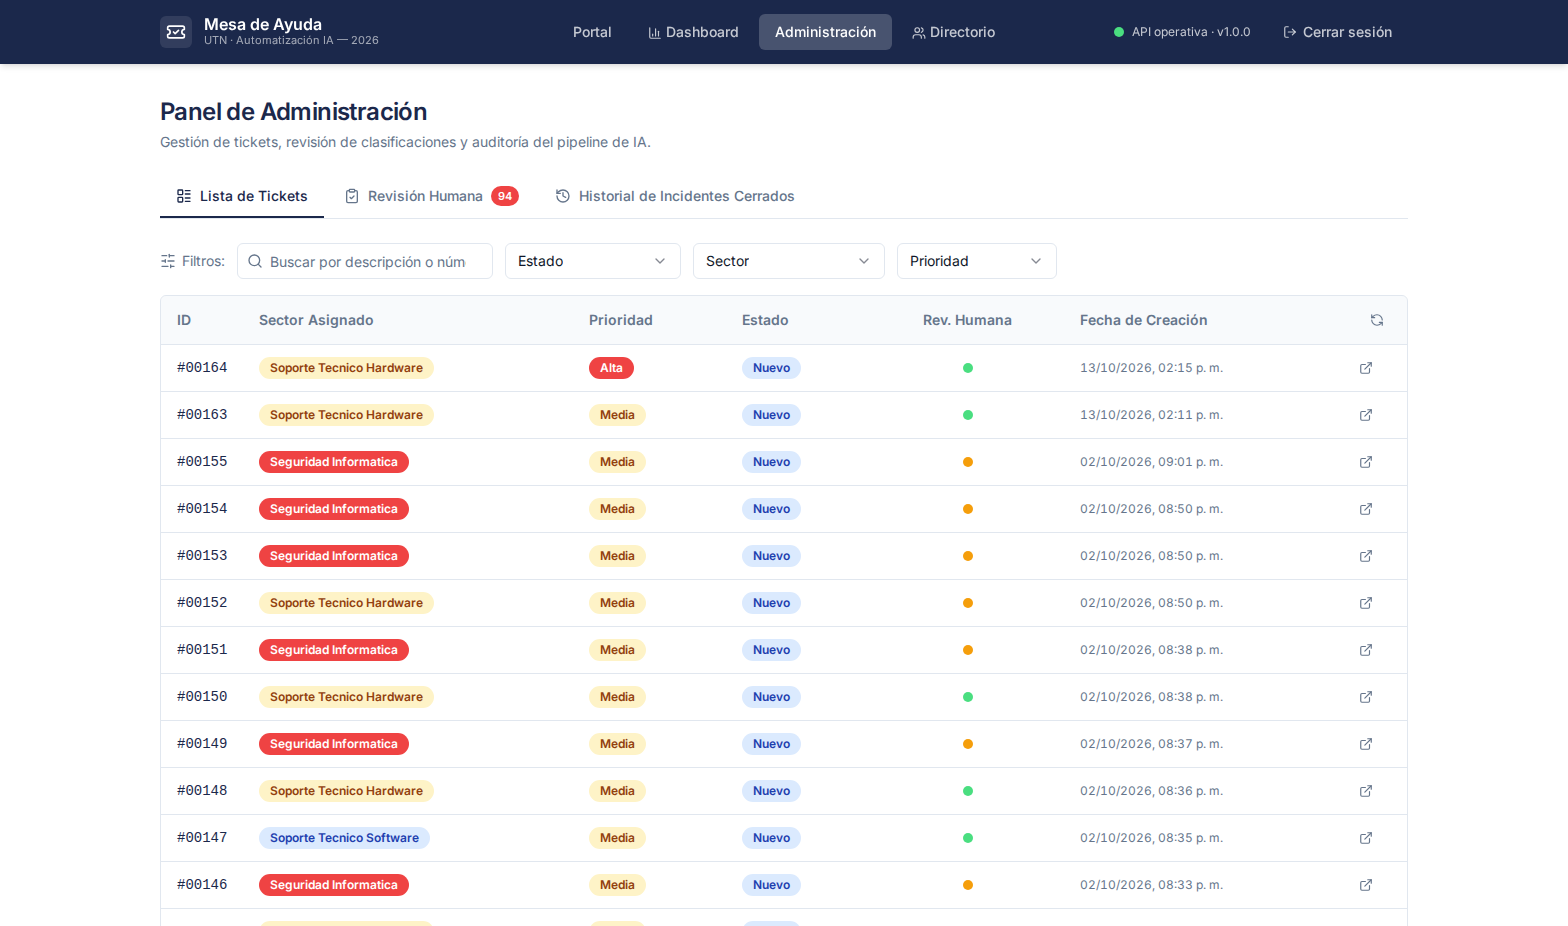
\includegraphics[width=\textwidth]{panel_admin}
\caption{Panel de administración del sistema: listado de tickets con filtros combinados y cola de revisión humana.}
\label{fig:panel_admin}
\end{figure}

El dashboard se organiza en tres visualizaciones principales. Un gráfico de tendencias muestra la evolución temporal de los incidentes, agrupables por día o por mes según la granularidad seleccionada por el operador. Un gráfico de torta presenta la distribución proporcional de incidentes entre los cinco sectores responsables. Un gráfico de barras apiladas desglosa los incidentes según su estado en el ciclo de vida, facilitando la identificación de cuellos de botella en la resolución. La Figura~\ref{fig:dashboard} presenta estas tres visualizaciones junto con los indicadores agregados del período seleccionado.

\begin{figure}[htbp]
\centering
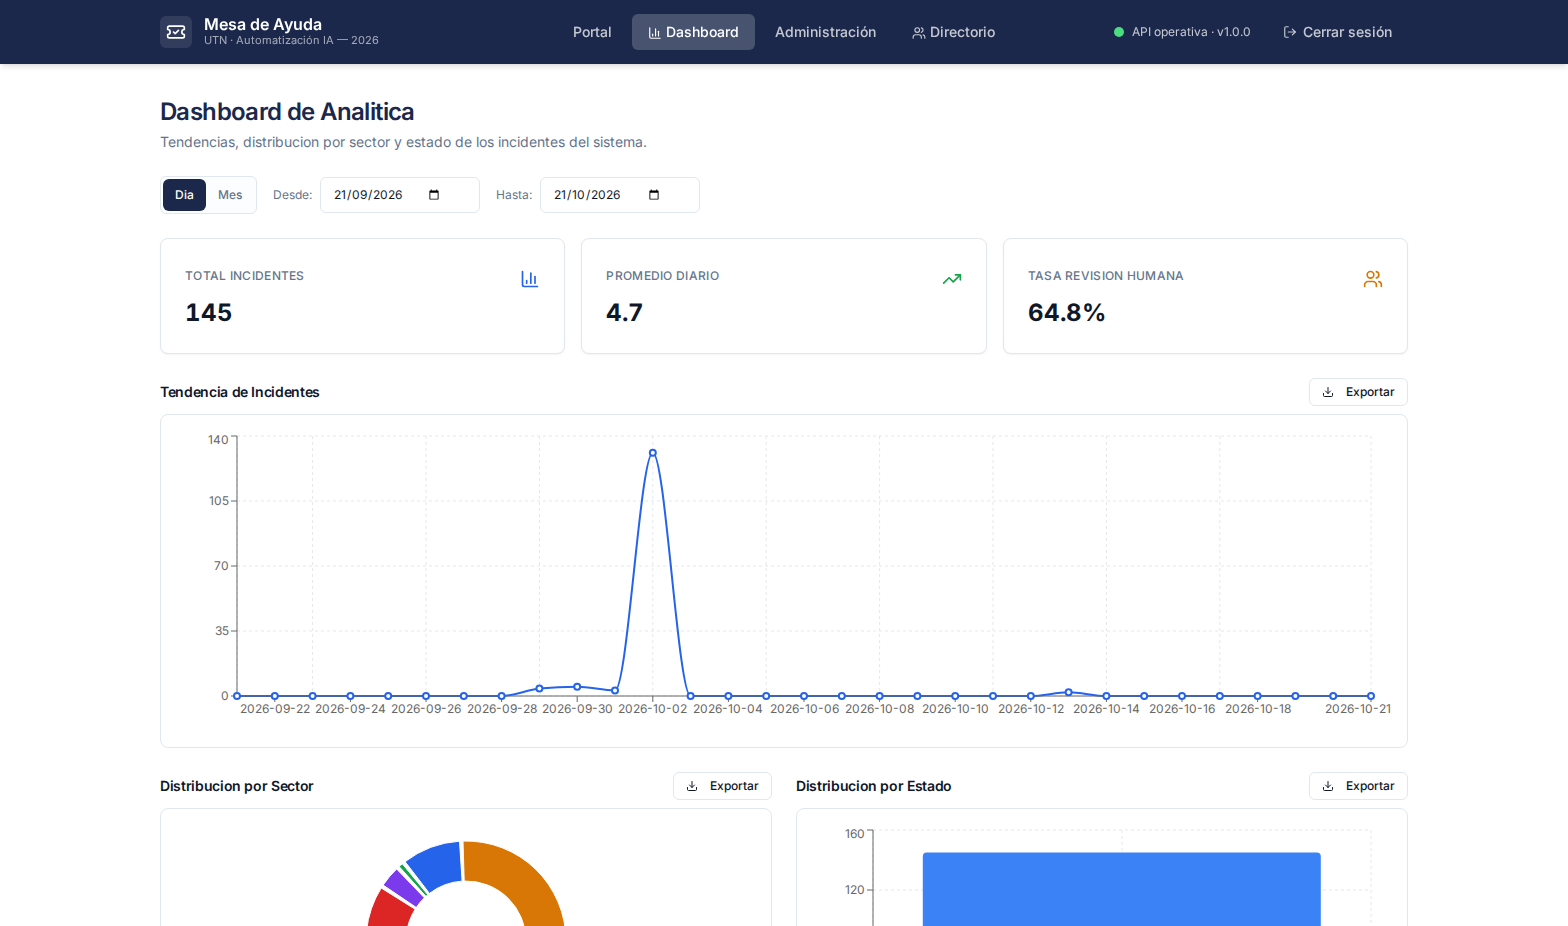
\includegraphics[width=\textwidth]{dashboard}
\caption{Dashboard de analítica del panel de administración: tendencia temporal de incidentes, distribución por sector y distribución por estado.}
\label{fig:dashboard}
\end{figure}

Los controles de filtro permiten acotar el período de análisis mediante un rango de fechas configurable, y alternar entre agrupación diaria y mensual para adaptar la granularidad al horizonte temporal de interés. Cada gráfico puede exportarse como imagen PNG para su inclusión en informes periódicos o presentaciones.

La utilidad práctica del dashboard puede ilustrarse con un escenario hipotético: si el sistema detectara que veinte usuarios reportaron la rotura de auriculares en una franja temporal acotada, el patrón sugeriría un problema de calidad del proveedor antes que una serie de fallas aisladas. Esta capacidad de identificar causas raíz a partir de datos agregados constituye un salto cualitativo respecto del enfoque tradicional de gestión de incidentes, donde cada ticket se trata de forma aislada y los patrones sistémicos permanecen invisibles.

\newpage


% --- Capitulo 7: Consideraciones eticas y legales (reubicado por c-105) ---
%==============================================================================
% Capítulo 7: Consideraciones éticas y aspectos legales (reubicado por c-105)
%==============================================================================
\section{Consideraciones éticas y aspectos legales}\label{sec:aspectos-legales}

\subsection{Marco normativo aplicable}\label{subsec:marco-normativo}

El sistema desarrollado se enmarca normativamente en la Ley~25.326 de Protección de los Datos Personales de la República Argentina \parencite{Ley25326_2000}, en su decreto reglamentario, el Decreto~1558/2001 \parencite{Decreto1558_2001}, y en las disposiciones complementarias emitidas por la Agencia de Acceso a la Información Pública en su carácter de autoridad de aplicación. Dado que el sistema realiza transferencia de fragmentos textuales hacia infraestructura de inferencia operada por proveedores con sede en los Estados Unidos, resultan aplicables las consideraciones del artículo 12 de la mencionada ley sobre transferencia internacional de datos personales y, de manera complementaria, los lineamientos del Reglamento General de Protección de Datos de la Unión Europea \parencite{GDPR2016} en aquellos casos que pudieran involucrar a residentes europeos. La Unión Europea reconoce a la Argentina como país con nivel adecuado de protección de datos personales mediante la Decisión 2003/490/CE, del 30 de junio de 2003, revalidada en enero de 2024. Esta adecuación ampara el flujo desde la Unión Europea hacia la Argentina y no opera en sentido inverso: los Estados Unidos no revisten la condición de país adecuado para la normativa argentina, de modo que la transferencia desde la Argentina hacia los proveedores de inferencia y de telefonía con sede en ese país requiere un instrumento específico conforme al artículo 12 de la Ley~25.326, según se detalla en la \autoref{subsec:transferencia-internacional}.

\subsection{Principios aplicados al tratamiento de datos}\label{subsec:principios-datos}

El diseño se atiene a cinco principios del tratamiento de datos personales. La licitud se funda en el artículo~5, inciso~2, apartado~d) de la Ley~25.326, que admite tratar los datos que deriven de una relación contractual, científica o profesional y resulten necesarios para su cumplimiento: la organización es la empleadora y trata datos de sus propios empleados para gestionar los incidentes que estos reportan. Esta base se distingue del consentimiento analizado para el corpus académico en la \autoref{subsec:consentimiento-derechos} y no dispensa el deber de información del artículo~6 de la Ley~25.326. La finalidad determinada limita el uso de los datos a la declaración y derivación de incidentes, sin usos secundarios no compatibles. La minimización se materializa en que solo se almacena el usuario corporativo y un directorio acotado ---legajo, nombre, correo electrónico corporativo, teléfono, sector y rol--- para resolver el contacto y notificar al usuario, descartando otros datos capturados incidentalmente (domicilios, documentos, información financiera). La exactitud opera mediante la revisión y corrección del incidente antes de su persistencia definitiva; el ejercicio de los derechos de rectificación, actualización y supresión (derechos ARCO) se resuelve en cinco días hábiles, de acuerdo con el artículo~16 de la Ley~25.326. La limitación del plazo de conservación fija una retención de 12 meses rodantes para los incidentes, justificada por el ciclo estadístico anual, independiente de la retención de 30 días de los registros de ejecución con fines de auditoría y diagnóstico (\autoref{subsec:capa-orquestacion}); los datos del directorio se conservan mientras la relación laboral permanezca activa y hasta un año después de su finalización, y luego se eliminan. Vencido el plazo, los datos del incidente se someten a anonimización irreversible, de modo que se eliminan los identificadores que permiten vincularlos a una persona. El bloqueo de escritura sobre los incidentes cerrados, que rechaza con un error 409 los intentos de modificación, constituye un control de integridad de auditoría y no una excepción permanente al vencimiento del plazo. La pseudonimización y el cifrado en reposo protegen la información durante el plazo de conservación declarado.

\subsection{Transferencia internacional y pseudonimización}\label{subsec:transferencia-internacional}

El tratamiento comporta dos transferencias internacionales hacia proveedores con sede en los Estados Unidos. La primera corresponde a la inferencia Gemini~3.6 Flash, a la que se envían fragmentos textuales descriptivos de los incidentes; sobre ese texto, el módulo Python local pseudonimiza los nombres propios, las direcciones de correo electrónico, los números telefónicos, los identificadores corporativos y los nombres de hosts internos con etiquetas genéricas como \texttt{[PERSONA]}, \texttt{[EMAIL]} o \texttt{[HOST]}, de modo que el texto transmitido no contiene identificadores directos. La pseudonimización se valida con expresiones regulares del dominio y pruebas unitarias dedicadas.

La segunda corresponde al canal telefónico de Twilio, con sede en los Estados Unidos: el llamante deja su solicitud y Twilio graba el audio; el audio crudo y el número telefónico se transfieren a la infraestructura del proveedor y se transcriben mediante reconocimiento del habla; recién después el backend pseudonimiza el texto ya transcrito. En consecuencia, el audio crudo y el número telefónico cruzan a los Estados Unidos antes de cualquier pseudonimización, que opera únicamente sobre el texto y no sobre el audio.

Ambas transferencias se dirigen a un país que no reviste la condición de adecuado para la normativa argentina, por lo que requieren un instrumento específico conforme al artículo 12 de la Ley~25.326: el consentimiento del titular o la suscripción de cláusulas contractuales modelo. El acuerdo de procesamiento de datos suscripto con cada proveedor complementa ese instrumento, pero no lo sustituye, en tanto no configura por sí mismo una de las bases de transferencia que la ley admite.

\subsection{Seguridad técnica}\label{subsec:seguridad-tecnica}

Las medidas de seguridad técnica del sistema se sustentan en la triada confidencialidad, integridad y disponibilidad (CIA) descrita por \textcite{Stallings2017_computer_security}, y su evidencia de control se sintetiza en la \autoref{tab:cumplimiento-iso} (tema Tecnológico). El cifrado en reposo con Fernet (AES-128 en modo CBC con HMAC-SHA-256), el cifrado en tránsito sobre TLS~1.2/1.3 en el borde, el control de acceso por rol, el registro de auditoría de las modificaciones, la gestión de credenciales por variables de entorno y las medidas de disponibilidad ---respaldo diario cifrado con prueba de restauración, contenedores con reinicio automático y monitoreo de salud--- quedan mapeados allí junto con sus brechas residuales. La capa TLS 1.2/1.3 se verifica de forma automatizada sobre el despliegue de referencia de la release v1.2.2, capacidad de la configuración entregada y no de la evaluada (Anexo~B, Tabla~\ref{tab:configuracion-evaluada-entregada}); la campaña experimental usó dos despliegues: la medición telefónica del 5 y 6 de octubre de 2026 corrió sobre el perfil aislado \texttt{corpus}, que no incluye el proxy inverso, mientras que la ingesta del 2 de octubre corrió sobre el stack base, que sí lo incluye; en ningún caso las mediciones dependen de TLS.

\subsection{Consentimiento, derechos del usuario y supervisión humana}\label{subsec:consentimiento-derechos}

Los usuarios de la organización son informados, mediante una política de privacidad accesible desde los canales de entrada, sobre las características del sistema, los datos que se recolectan, la transferencia internacional aplicable y los derechos que les asisten conforme a la normativa vigente. Se garantiza el ejercicio de los derechos de acceso, rectificación, actualización y supresión (derechos ARCO) mediante un procedimiento documentado a cargo del responsable de protección de datos designado por la organización.

En lo que respecta al consentimiento informado para los fines de investigación académica, los 120 empleados de la organización fueron notificados mediante comunicación interna formal, con descripción explícita del propósito del estudio, del tipo de datos tratados, del carácter pseudonimizado de los registros y del derecho a requerir la exclusión de sus incidentes del corpus de validación. El procedimiento fue supervisado por la dirección académica del trabajo y avalado institucionalmente mediante una carta de autorización emitida por la organización adoptante.

En relación con el protocolo de medición en vivo aplicado durante la fase experimental ---en el cual los dos operadores se cronometraron mutuamente y sabían que se registraban tiempos, sin que se les anunciaran el inicio de cada medición ni el propósito comparativo del estudio, con el objeto de atenuar el efecto Hawthorne, de modo que la información sobre ese propósito fue diferida---, corresponde dejar constancia de que, una vez concluida la recolección de datos, se realizó una sesión de esclarecimiento posterior (\textit{debriefing}) con los dos operadores participantes. En dicha sesión se explicó el propósito del estudio, se detalló el procedimiento de medición empleado y se ofreció a cada operador la posibilidad de solicitar la exclusión de sus registros individuales del corpus de validación. Ninguno de los operadores ejerció este derecho. Este procedimiento se alinea con las recomendaciones de la Asociación Americana de Psicología para investigaciones que emplean medición con información diferida sobre el propósito del estudio \parencite{APA2017}, y fue supervisado por el director del trabajo.

En concordancia con las recomendaciones contemporáneas sobre sistemas que incorporan inteligencia artificial, se preserva en todo momento la posibilidad de supervisión humana significativa. Ninguna decisión que afecte derechos sustanciales de los usuarios se toma de manera completamente automatizada sin posibilidad de revisión, y el sector responsable conserva la potestad de modificar la clasificación inicial cuando lo considere apropiado, registrándose tal modificación en la tabla de trazabilidad descrita en la \autoref{sec:arquitectura}. Este mecanismo materializa el principio de la persona en el bucle (\emph{human in the loop}) como salvaguarda frente a errores potenciales del clasificador automático. Cabe precisar su alcance: el umbral de confianza de 0,70 que dispara la revisión obligatoria se evalúa solo sobre la salida de la etapa Gemini (la etapa de reserva deriva siempre a revisión, con confianza 0,0), de modo que sobre el 65,5~\% de los casos, resueltos por la etapa determinística, no existe derivación automática por caso basada en la clasificación; desde el 13 de octubre de 2026, posterior a las corridas de la campaña, el backend deriva además a revisión el incidente cuyo reportante no se identifica en el directorio de empleados, condición independiente de la clasificación. Para esa fracción la salvaguarda se limita al criterio con que se fijó el punto de operación del filtro ---precisión no inferior a la del modelo sobre el conjunto que resuelve, estimada sobre el corpus de validación--- y a la reasignación trazable del incidente descrita, disponible en la interfaz REST y expuesta en la interfaz web solo para los casos derivados. El análisis de calibración por etapa muestra que la confianza de Gemini no discrimina aciertos de errores en su rango observado (0,85 a 1,00) y que la etapa de reglas no emite una confianza utilizable para derivar (\autoref{subsec:calibracion}); el umbral de 0,70 no garantiza, por lo tanto, la detección de errores.

\subsection{Cumplimiento normativo y alineación con estándares}\label{subsec:cumplimiento}

\subsubsection{Marco de referencia adoptado}\label{subsec:cumplimiento-marco}

Este apartado evalúa el grado de alineación del sistema con los marcos adoptados: ISO/IEC~27001:2022 \parencite{ISO27001_2022} y su catálogo de controles ISO/IEC~27002:2022 \parencite{ISO27002_2022}, NIST CSF~2.0 \parencite{NIST2024_csf}, la norma de gestión de la privacidad ISO/IEC~27701:2025 \parencite{ISO27701_2025} y la Ley~25.326. El relevamiento es estático y documental: describe el grado de alineación y las brechas identificadas, no un aseguramiento de un tercero (no constituye una acreditación externa ni una auditoría independiente), y su detalle se conserva en el repositorio (\texttt{docs/cumplimiento/}).

\subsubsection{Estado de alineación con ISO/IEC 27002:2022}\label{subsec:cumplimiento-iso}

La Tabla~\ref{tab:cumplimiento-iso} agrupa por tema los controles de ISO/IEC~27002:2022, que corresponden al Anexo~A de ISO/IEC~27001:2022; el inventario de los 93 controles reside en el repositorio.

\begin{table}[htbp]
\centering
\caption{Estado de alineación con los controles de ISO/IEC 27002:2022, agrupados por tema}
\label{tab:cumplimiento-iso}
\footnotesize\singlespacing
\setlength{\tabcolsep}{4pt}
\begin{tabular}{@{}>{\raggedright\arraybackslash}p{2.2cm} >{\raggedright\arraybackslash}p{1.4cm} >{\raggedright\arraybackslash}p{1.7cm} >{\raggedright\arraybackslash}p{10.5cm}@{}}
\toprule
\textbf{Tema} & \textbf{Controles} & \textbf{Estado} & \textbf{Evidencia / brecha principal} \\
\midrule
Organizacional & 5.x & Parcial & Política, clasificación, roles e IR (C-61); residual: revisión independiente (5.35) \\
Personas & 6.x & No aplicable & Selección, formación, sanciones y cese: competen al adoptante \\
Físico & 7.x & No aplicable & Sin infraestructura productiva; se cubren en el hosting del adoptante \\
Tecnológico & 8.x & Alineado y parcial & Pseudonimización, Fernet, TLS, JWT y roles, vulnerabilidades en CI y respaldo cifrado (C-62 a C-66), MFA de cuentas privilegiadas (C-63b); residual: operación con KMS/PAM, logs centralizados y redundancia offsite \\
\bottomrule
\end{tabular}
\par
{\footnotesize\textit{Fuente:} elaboración propia a partir del gap assessment ISO/IEC 27001:2022/27002:2022 y NIST CSF 2.0.\par}
\end{table}

\subsubsection{Perfil de alineación con NIST CSF 2.0}\label{subsec:cumplimiento-nist}

La Tabla~\ref{tab:cumplimiento-nist} cubre las seis funciones de NIST CSF~2.0 y su madurez en una escala propia del relevamiento, de 0 (inexistente) a 4 (optimizado).

\begin{table}[htbp]
\centering
\caption{Perfil de alineación con las funciones de NIST CSF 2.0}
\label{tab:cumplimiento-nist}
\footnotesize\singlespacing
\setlength{\tabcolsep}{4pt}
\begin{tabular}{@{}>{\raggedright\arraybackslash}p{2.2cm} >{\raggedright\arraybackslash}p{3.7cm} >{\centering\arraybackslash}p{1.2cm} >{\raggedright\arraybackslash}p{8.7cm}@{}}
\toprule
\textbf{Función} & \textbf{Subcategoría representativa} & \textbf{Madurez} & \textbf{Brecha principal} \\
\midrule
GV (Gobernar) & Políticas, roles, riesgo y proveedores & 2 & Política, roles y evaluación de proveedores vigentes (C-61, C-64); residual: revisión independiente del adoptante (5.35) \\
ID (Identificar) & Inventario de activos y clasificación & 2 & Inventario de activos y clasificación y etiquetado vigentes (C-61; 5.9, 5.12, 5.13); residual: SBOM del adoptante \\
PR (Proteger) & Acceso, endurecimiento y criptografía & 3 & Pseudonimización, Fernet, TLS, JWT y roles, MFA de cuentas privilegiadas y SAST/auditoría de dependencias en CI (C-62 a C-64); residual: KMS/PAM y SIEM del adoptante (8.5, 8.8, 8.20, 8.24) \\
DE (Detectar) & Monitoreo y detección de eventos & 1 & Logs estructurados, chequeos de salud y retención por clase (C-66; 8.15 parcial); sin centralización ni alertas de seguridad (brecha 8.16) \\
RS (Responder) & Plan de respuesta y mitigación & 2 & Plan de respuesta a incidentes vigente (C-61; 5.24--5.27) y manejo de evidencia (5.28 parcial, C-156); residual: operación en producción del adoptante \\
RC (Recuperar) & Recuperación y restauración & 2 & Respaldo cifrado y continuidad con RTO/RPO; copia fuera del host y redundancia como acción del adoptante (5.29, 5.30, 8.13, 8.14) \\
\bottomrule
\end{tabular}
\par
{\footnotesize\textit{Fuente:} elaboración propia a partir del gap assessment ISO/IEC 27001:2022/27002:2022 y NIST CSF 2.0 (\texttt{docs/cumplimiento/gap-assessment-iso27001-27002-nist-csf2.md}, sección~4), con el estado reconciliado al 28-10-2026 (release \texttt{v1.2.5}).\par}
\end{table}

\subsubsection{Brechas principales y hoja de ruta}\label{subsec:cumplimiento-brechas}

Los seis changes de cumplimiento cerraron, para el alcance del repositorio, las brechas priorizadas: C-61 (gobernanza documental: 5.1, 5.2, 5.9, 5.12, 5.13, 5.24--5.27, 5.31, 8.26), C-62 (endurecimiento de red: 8.20, 8.22, 8.2, 5.14, 8.31), C-63 (identidades y accesos: 8.5, 5.15, 5.17, 8.2), C-64 (vulnerabilidades: 8.8, 8.28, 8.29, 5.19--5.23), C-65 (respaldo y continuidad: 8.13, 8.14, 5.29, 5.30, 5.33) y C-66 (privacidad: 5.34, 8.12, 8.15, 5.31). La MFA TOTP con desafío para cuentas privilegiadas y la rotación de claves (secreto JWT y clave Fernet) quedaron implementadas en el repositorio (C-63a/b/c, archivados el 2026-10-08); su operación con KMS/PAM, la custodia de claves en producción, la centralización de logs, la redundancia fuera del host y el SBOM quedan como acción de la organización adoptante; las brechas organizacionales ---personas (6.x), físicas (7.x), revisión independiente (5.35), segregación de funciones (5.3) y trabajo remoto (6.7, 8.1)--- son responsabilidad de la organización adoptante.

\subsubsection{Alineación con el marco legal}\label{subsec:cumplimiento-legal}

El plano legal de la alineación se desarrolla en el \autoref{subsec:marco-normativo} y en la \autoref{subsec:transferencia-internacional}, a los que este apartado remite sin reproducir su contenido. Los controles de privacidad mapeados (5.31, 5.34, 8.12, 8.15) se apoyan en la base de licitud del artículo~5 de la Ley~25.326, en el instrumento de transferencia internacional del artículo~12 y en los plazos ARCO del artículo~16.

\newpage


% --- Capitulo 8: Resultados ---
%==============================================================================
% Capítulo 8: Resultados
%==============================================================================
\section{Resultados}\label{sec:resultados}

Este capítulo presenta los resultados de la validación experimental en cuatro dimensiones: tiempos de registro, desempeño de clasificación, reducción de la intervención humana y análisis cualitativo de errores.

\subsection{Comparación de tiempos de registro}\label{subsec:comparacion-tiempos}

La comparación de los tiempos de registro entre el flujo manual y el flujo automatizado se sintetiza en la Tabla~\ref{tab:tiempos}. La media aritmética del tiempo manual sobre los 200 casos del corpus fue de 61,6~s (mediana de 50,0~s), con un desvío estándar de 44,9~s y un rango entre 10 y 300~s. Este valor, respaldado por la planilla de cronometraje descrita en la \autoref{subsec:diseno-experimental}, corresponde a la medición experimental incidente por incidente y reemplaza a la estimación preliminar de 2 minutos con 45 segundos citada en la \autoref{subsec:planteamiento-problema}, obtenida sin cronometraje individual. La media del flujo automatizado fue de 17,76~s (mediana de 17,47~s), con un desvío estándar de 13,48~s y un rango entre 0,525 y 65,834~s. La reducción relativa de la media de tiempo alcanzó el 71,2~\%.

\begin{table}[htbp]
\centering
\caption{Estadísticos descriptivos de los tiempos de registro por flujo (\(n = 200\))}
\label{tab:tiempos}
\small
\begin{tabular}{@{}>{\raggedright\arraybackslash}p{4.0cm} p{3.5cm} p{3.5cm} p{2.5cm}@{}}
\toprule
\textbf{Estadístico} & \textbf{Flujo manual} & \textbf{Flujo automatizado} & \textbf{Reducción} \\
\midrule
Media aritmética (s)      & 61,6   & 17,76   & 71,2~\% \\
Mediana (s)               & 50,0   & 17,47   & 65,1~\% \\
Desvío estándar (s)       & 44,9   & 13,48   & --- \\
Mínimo (s)                & 10     & 0,525   & --- \\
Máximo (s)                & 300    & 65,834  & --- \\
\bottomrule
\end{tabular}
\par\smallskip
{\footnotesize\textit{Fuente:} elaboración propia a partir del corpus de validación (\(n = 200\)).\par}
\end{table}

El tiempo automatizado de registro desagregado por canal de origen se presenta en la Tabla~\ref{tab:tiempos-canal}. El canal telefónico incorpora, además de la latencia de procesamiento, la duración de la llamada grabada; como la grabación esta acotada a un máximo de 45~s (véase la \autoref{subsec:metricas-instrumentos}), su valor constituye una cota inferior de la duración real de la llamada.

\begin{table}[htbp]
\centering
\caption{Tiempo automatizado de registro por canal de origen (\(n = 200\))}
\label{tab:tiempos-canal}
\small
\begin{tabular}{@{}p{6.0cm} c c c@{}}
\toprule
\textbf{Canal de origen} & \textbf{Casos} & \textbf{Media (s)} & \textbf{Mediana (s)} \\
\midrule
Llamada telefónica (cota inferior) & 81 & 20,09 & 18,70 \\
Correo electrónico                 & 66 & 27,65 & 25,82 \\
Formulario web                     & 53 & 1,88  & 1,26  \\
\midrule
\textbf{Global}                    & \textbf{200} & \textbf{17,76} & \textbf{17,47} \\
\bottomrule
\end{tabular}
\par\smallskip
{\footnotesize\textit{Fuente:} elaboración propia a partir del corpus de validación (\(n = 200\)).\par}
\end{table}

La prueba de Wilcoxon de rangos con signo aplicada sobre las mediciones pareadas \parencite{Virtanen2020_scipy} arrojó un estadístico de contraste \(W = \min(T^{+}, T^{-}) = 363\), con una suma de rangos positivos \(T^{+} = 19.737\), una suma de rangos negativos \(T^{-} = 363\) y \(n = 200\) pares válidos, junto con un valor \(p = 3{,}08 \times 10^{-32}\), lo que permite rechazar la hipótesis nula de igualdad de medianas con un nivel de confianza superior al 99,9~\%. El estadístico refleja que en 188 de los 200 pares el flujo automatizado fue más veloz que el manual; en los 12 pares restantes (6,0~\%) el flujo automatizado no fue más rápido, resultado coherente con la diferencia de aproximadamente 32,5~s entre medianas. La prueba se eligió por el rechazo de la normalidad en los tres conjuntos de tiempos (\autoref{subsec:analisis-estadistico}).

Para cuantificar la magnitud práctica de la diferencia, se calculó el coeficiente \(r\) de correlación rank-biserial a partir de los dos estadísticos de rango:
\[
r = \frac{T^{+} - T^{-}}{n(n+1)/2} = \frac{19.737 - 363}{200 \cdot 201 / 2} = \frac{19.374}{20.100} = 0{,}9639
\]
El valor obtenido (\(r = 0{,}9639\)) corresponde a un tamaño del efecto muy alto. La diferencia observada es, por tanto, estadísticamente significativa y, dada su magnitud absoluta, relativa y el tamaño del efecto reportado, también prácticamente relevante para la operación.

Cabe señalar que el tiempo manual se registró con redondeo hacia arriba (véase la \autoref{subsec:diseno-experimental}), un sesgo de medición sistemático que infla la línea base manual. Por ese motivo la reducción del 71,2~\% debe leerse como cota superior. Un análisis de sensibilidad que descuenta 5~s y 10~s a cada medición manual reduce la media manual a 56,6~s y 51,6~s, respectivamente, y sitúa la reducción en el 68,6~\% y en el 65,6~\% como cota inferior conservadora. Aun en el escenario más desfavorable la reducción de tiempo permanece sustancial y estadísticamente significativa (\(p = 1{,}8 \times 10^{-26}\), \(r = 0{,}8683\)).

\begin{figure}[htbp]
\centering
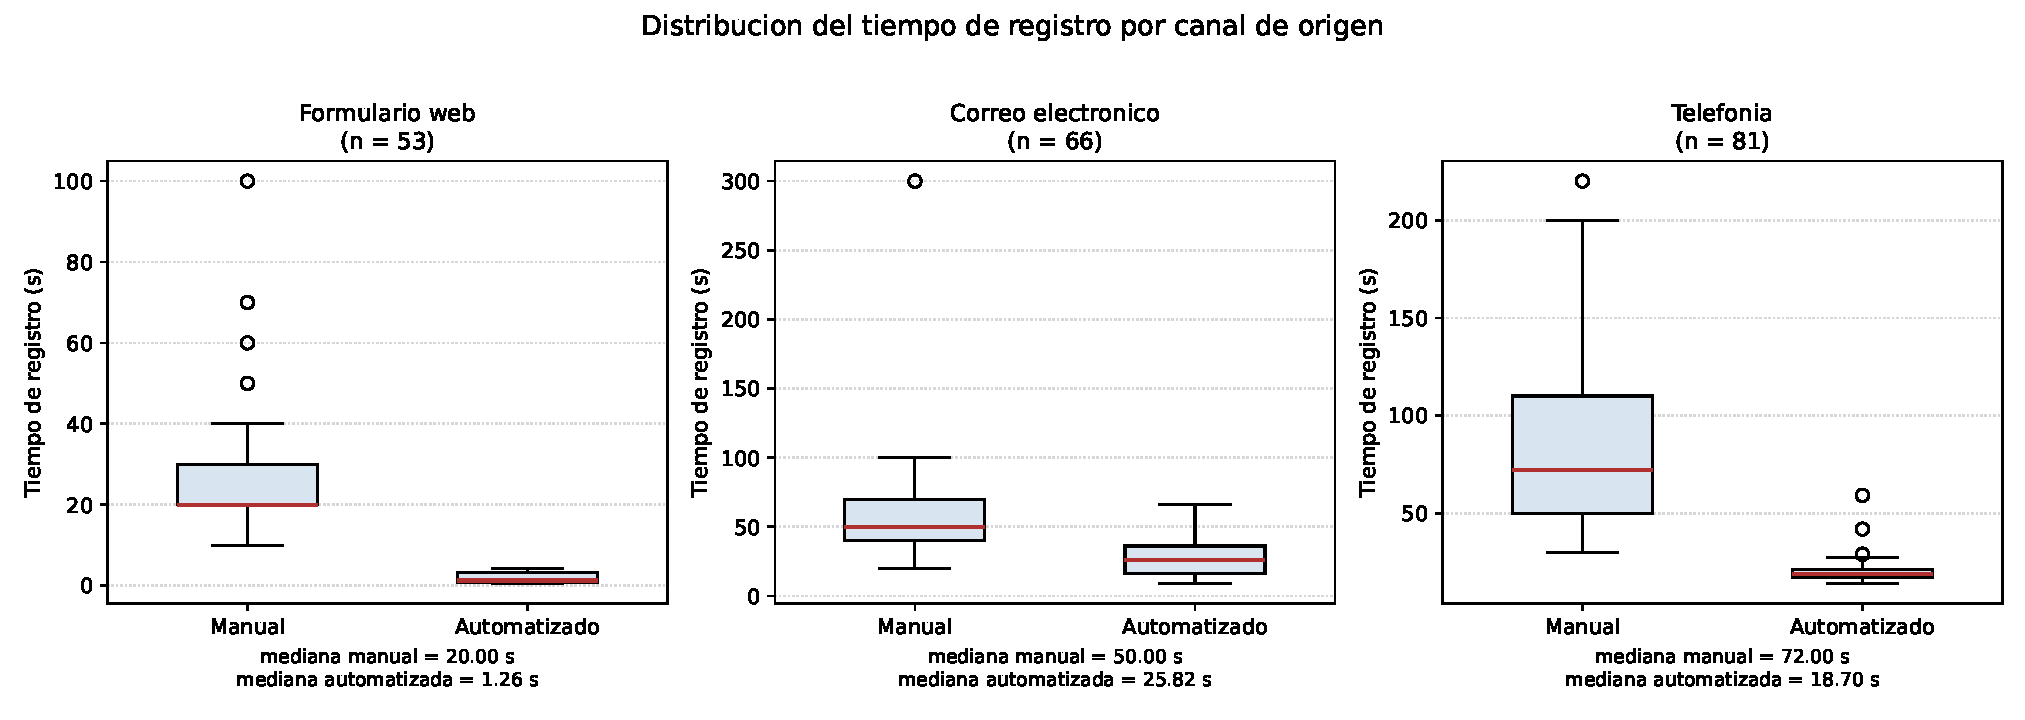
\includegraphics[width=\textwidth]{boxplot_tiempos}
\caption{Distribución del tiempo de registro por canal de origen (manual frente a automatizado). El panel de telefonía incorpora la duración de la llamada grabada.}
\label{fig:boxplot_tiempos}
\end{figure}

\subsection{Matriz de confusión y métricas de clasificación}\label{subsec:matriz-metricas}

La evaluación de clasificación se realizó sobre el corpus real de 200 casos pseudonimizados, cuya distribución por sector y por canal se describe en la \autoref{subsec:poblacion-muestra-corpus}.

La matriz de confusión obtenida se presenta en la Tabla~\ref{tab:matriz} y en la Figura~\ref{fig:matriz_confusion}. La exactitud estricta resultante asciende al 73,5~\% (147 casos correctos sobre 200).

\begin{table}[htbp]
\centering
\caption{Matriz de confusión del clasificador automático (\(n = 200\)). Filas: sector asignado; columnas: sector predicho principal.}
\label{tab:matriz}
\small
\setlength{\tabcolsep}{4pt}
\begin{tabular}{@{}>{\raggedright\arraybackslash}p{2.6cm} *{5}{>{\centering\arraybackslash}p{1.85cm}} >{\centering\arraybackslash}p{1.3cm}@{}}
\toprule
\textbf{Asignado \(\backslash\) Predicho} & \textbf{Seguridad Informatica} & \textbf{Soporte Tecnico Hardware} & \textbf{Soporte Tecnico Software} & \textbf{Bases de Datos} & \textbf{Sistemas} & \textbf{Total} \\
\midrule
Seguridad Informatica & 15 & 2 & 11 & 2 & 1 & \textbf{31} \\
Soporte Tecnico Hardware & 1 & \textbf{77} & 3 & 0 & 4 & \textbf{85} \\
Soporte Tecnico Software & 0 & 11 & \textbf{48} & 1 & 7 & \textbf{67} \\
Bases de Datos & 0 & 0 & 1 & 0 & 0 & \textbf{1} \\
Sistemas & 2 & 0 & 5 & 2 & \textbf{7} & \textbf{16} \\
\midrule
\textbf{Total} & \textbf{18} & \textbf{90} & \textbf{68} & \textbf{5} & \textbf{19} & \textbf{200} \\
\bottomrule
\end{tabular}
\par\smallskip
{\footnotesize\textit{Fuente:} elaboración propia a partir del corpus de validación (\(n = 200\)).\par}
\end{table}

\begin{figure}[htbp]
\centering
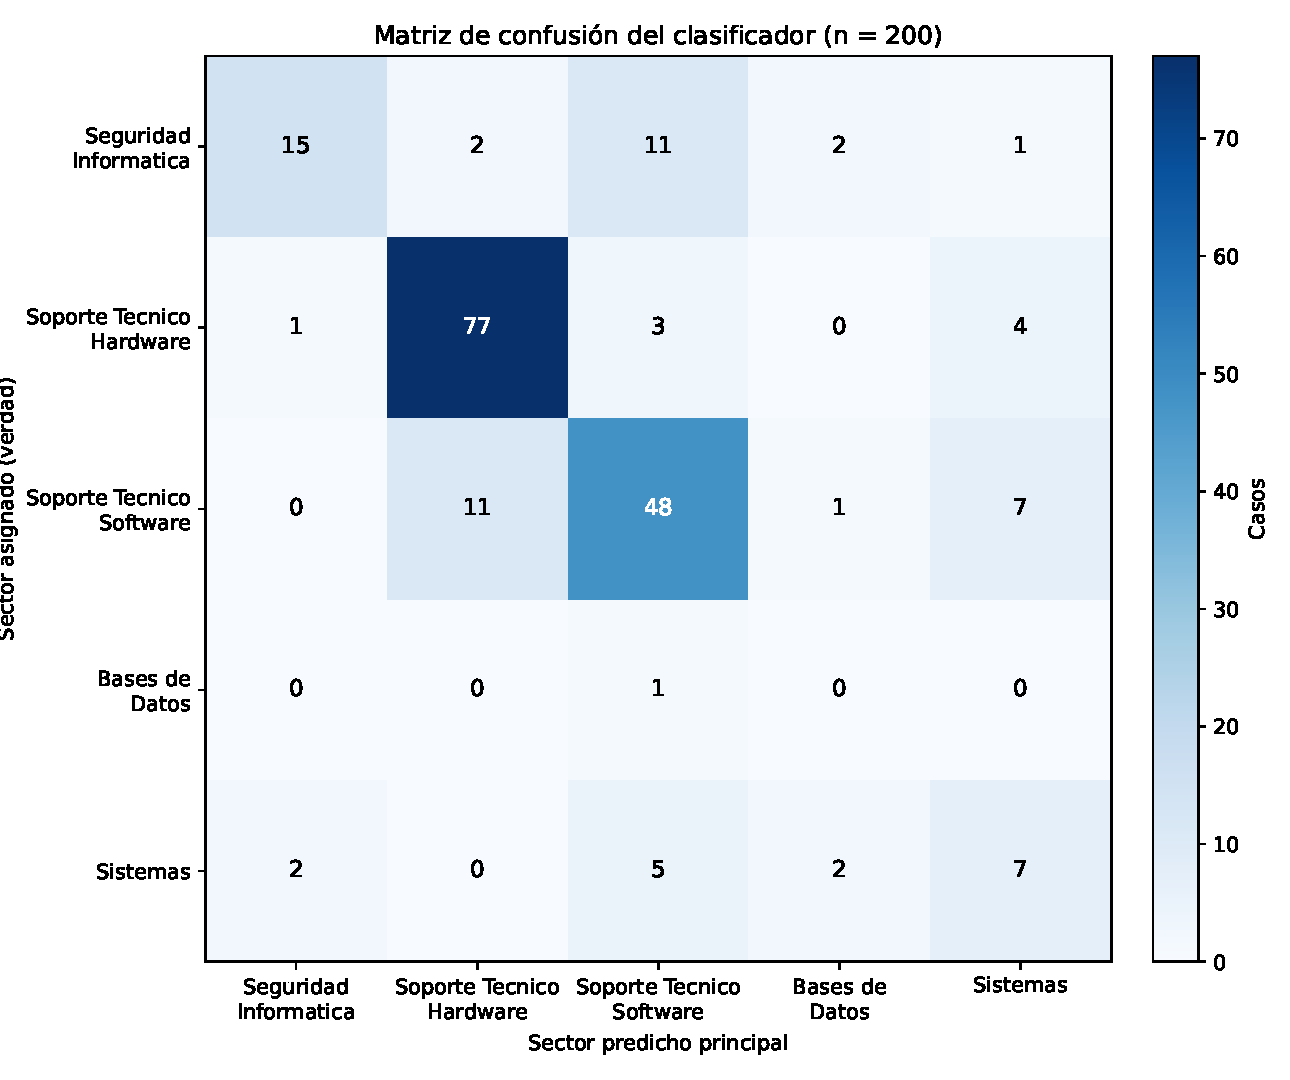
\includegraphics[width=0.85\textwidth]{matriz_confusion}
\caption{Matriz de confusión del clasificador (\(n = 200\)). Filas: sector asignado (verdad); columnas: sector predicho principal.}
\label{fig:matriz_confusion}
\end{figure}

Los valores de precisión, sensibilidad (recall) y F1 por clase, con su intervalo de confianza al 95~\% \parencite{Sokolova2009_performance_measures}, se presentan en la Tabla~\ref{tab:metricas}. La evaluación se enmarca en un único marco métrico cuya referencia de verdad es multietiqueta (107 de los 200 casos, 53,5~\%), frente a una salida del clasificador de una etiqueta principal: la exactitud estricta del 73,5~\% (147/200) es la métrica primaria monoetiqueta, con IC de Wilson al 95~\% de [67,0~\%, 79,1~\%]. El macro-F1 de umbral se reporta sobre las cuatro clases estimables (0,6508), excluida Bases de Datos (\(n = 1\), no estimable), y el de cinco clases (0,5207) se conserva como valor informativo. Las métricas secundarias se calculan contra el conjunto de verdad del corpus (multietiqueta): subset accuracy 0,43 (IC [0,36; 0,50]), Hamming loss 0,3586 (IC [0,31; 0,41]) y micro-F1 0,6654 (IC [0,62; 0,71]). Estas métricas de conjunto penalizan estructuralmente una salida forzada a una sola etiqueta y no son equivalentes de la exactitud estricta: el micro-F1 acumula los aciertos por etiqueta y no por caso, de modo que su valor (0,6654) no debe leerse como una exactitud (0,7350). De los 200 casos, 131 fueron resueltos por la etapa determinística del clasificador y 69 requirieron la etapa Gemini.

\begin{table}[htbp]
\centering
\caption{Métricas de clasificación por clase con intervalo de confianza al 95~\% (una contra el resto)}
\label{tab:metricas}
\small
\setlength{\tabcolsep}{4pt}
\begin{tabular}{@{}>{\raggedright\arraybackslash}p{4.5cm} >{\centering\arraybackslash}p{3.4cm} >{\centering\arraybackslash}p{3.4cm} >{\centering\arraybackslash}p{3.4cm}@{}}
\toprule
\textbf{Clase} & \textbf{Precisión (IC 95~\%)} & \textbf{Sensibilidad (IC 95~\%)} & \textbf{F1 (IC 95~\%)} \\
\midrule
Soporte Tecnico Hardware  & 0,8556 [0,77; 0,91] & 0,9059 [0,83; 0,95] & 0,8800 [0,82; 0,93] \\
Soporte Tecnico Software  & 0,7059 [0,59; 0,80] & 0,7164 [0,60; 0,81] & 0,7111 [0,61; 0,80] \\
Seguridad Informatica     & 0,8333 [0,61; 0,94] & 0,4839 [0,32; 0,65] & 0,6122 [0,44; 0,75] \\
Sistemas                  & 0,3684 [0,19; 0,59] & 0,4375 [0,23; 0,67] & 0,4000 [0,16; 0,59] \\
Bases de Datos            & \multicolumn{3}{c}{no estimable (\(n = 1\))} \\
\bottomrule
\end{tabular}
\par\smallskip
{\footnotesize\textit{Fuente:} elaboración propia a partir del corpus de validación (\(n = 200\)). IC de precisión y sensibilidad por Wilson; IC de F1 por bootstrap percentil (2000 remuestreos).\par}
\end{table}

Estas métricas confirman un desempeño desigual entre las clases objetivo \parencite{Sokolova2009_performance_measures}. Este desequilibrio importa en el contexto operativo, porque un clasificador que concentra sus errores en una clase minoritaria genera derivaciones erroneas en un sector específico y puede erosionar la confianza de ese equipo en la herramienta, independientemente de sus métricas agregadas.

La inspección de la matriz de confusión revela que los 53 errores totales se concentran en fronteras entre sectores léxicamente próximos, con Soporte Tecnico Software como categoría central; su análisis cualitativo, agrupado por frontera de confusión, se desarrolla en la \autoref{subsec:analisis-errores}.

\subsection{Intervención humana en el flujo automatizado}\label{subsec:reduccion-intervencion}

La intervención humana en el flujo automatizado se deriva del gate de revisión implementado, \texttt{requiere\_revision\_humana = (confianza < 0,70)}, que escala un caso a un operador humano cuando la confianza devuelta por el clasificador cae por debajo de ese umbral. El gate de revisión no derivó ningún caso del corpus: la etapa determinística fija el campo en \texttt{False} y la etapa Gemini nunca devolvió una confianza inferior a 0,85.

La sub-hipótesis de intervención humana por caso se declara no contrastada por ausencia de registro primario: la proporción no se computa como resultado, de modo que el aporte operativo asociado al gate queda, por lo tanto, como no medido.

\subsection{Calibración de la confianza}
\label{subsec:calibracion}

La confianza declarada por el clasificador solo resulta útil como criterio de derivación si guarda relación con la exactitud real. Para verificar esa relación se contrastó, sobre los 200 casos del corpus, la confianza devuelta en cada predicción contra la corrección de la clasificación. La Tabla~\ref{tab:bandas} desagrega la exactitud por bandas de confianza en torno al umbral del 70~\% que gobierna el gate de revisión humana.

\begin{table}[htbp]
\centering
\caption{Exactitud por banda de confianza declarada}
\label{tab:bandas}
\small
\begin{tabular}{@{}l c c c@{}}
\toprule
\textbf{Banda de confianza} & \textbf{Casos} & \textbf{Aciertos} & \textbf{Exactitud} \\
\midrule
\([0{,}00\,;\,0{,}50)\) & 98 & 75 & 0,765 \\
\([0{,}50\,;\,0{,}70)\) & 26 & 19 & 0,731 \\
\([0{,}70\,;\,0{,}85)\) & 6  & 2  & 0,333 \\
\([0{,}85\,;\,0{,}95)\) & 31 & 22 & 0,710 \\
\([0{,}95\,;\,1{,}00]\) & 39 & 29 & 0,744 \\
\bottomrule
\end{tabular}
\par\smallskip
{\footnotesize\textit{Fuente:} elaboración propia a partir del corpus de validación (\(n = 200\)).\par}
\end{table}

Los datos revelan una calibración invertida o anti-calibrada: los casos de confianza alta (\(\ge 0{,}70\)) fueron menos exactos (0,697) que los de confianza baja (\(< 0{,}70\), 0,758). La tendencia se acentúa en el extremo superior de la escala: dentro de los 46 casos con confianza igual o superior a 0,90 se registraron 13 errores (28,3~\%), y la banda \([0{,}70\,;\,0{,}85)\) alcanzó apenas 0,333 de exactitud. En otras palabras, el clasificador no solo no discrimina mejor cuando declara mayor certeza, sino que en los tramos de confianza más alta la exactitud se degrada. La consecuencia operativa es directa: el gate del 70~\% no aisló los errores, porque estos se distribuyen también en las bandas de confianza alta. Este hallazgo fundamenta la discusión de la \autoref{sec:discusion}.

\subsection{Análisis de errores y casos límite}\label{subsec:analisis-errores}

El análisis cualitativo de los 53 casos mal clasificados permitió identificar patrones de error recurrentes, agrupados por frontera de confusión y sintetizados en la Tabla~\ref{tab:errores}.

\begin{table}[htbp]
\centering
\caption{Confusiones observadas en la clasificación automática, por frontera}
\label{tab:errores}
\small
\begin{tabular}{@{}>{\raggedright\arraybackslash}p{8.5cm} p{2.0cm} p{2.5cm}@{}}
\toprule
\textbf{Frontera de confusión} & \textbf{Casos} & \textbf{Proporción} \\
\midrule
Soporte Tecnico Hardware \(\leftrightarrow\) Soporte Tecnico Software & 14 & 26,4~\% \\
Sistemas \(\leftrightarrow\) Soporte Tecnico Software & 12 & 22,6~\% \\
Seguridad Informatica \(\leftrightarrow\) Soporte Tecnico Software & 11 & 20,8~\% \\
Otras fronteras & 16 & 30,2~\% \\
\midrule
\textbf{Total} & \textbf{53} & \textbf{100~\%} \\
\bottomrule
\end{tabular}
\par\smallskip
{\footnotesize\textit{Fuente:} elaboración propia a partir del corpus de validación (\(n = 200\)).\par}
\end{table}

El patrón dominante, presente en 14 casos (26,4~\% de los errores), corresponde a la frontera entre Soporte Tecnico Hardware y Soporte Tecnico Software: incidentes en que una falla física de un equipo afecta a una aplicación, o en que una tarea sobre una aplicación se describe con términos de equipamiento, de modo que la decisión correcta depende del juicio humano sobre que aspecto prevalece. El segundo patrón, presente en 12 casos (22,6~\%), corresponde a la frontera entre Sistemas y Soporte Tecnico Software, asociada a acciones sobre servidores y servicios de plataforma descritas como problemas de una aplicación. El tercer patrón, presente en 11 casos (20,8~\%), corresponde a la frontera entre Seguridad Informatica y Soporte Tecnico Software, vinculada a incidentes de acceso y credenciales. El 30,2~\% restante se reparte entre las demas fronteras, incluidas las confusiones que involucran a Bases de Datos, con un único caso de soporte.

Los patrones anteriores se ilustran con tres casos mal clasificados del corpus. Las descripciones se reproducen pseudonimizadas y se acompañan con el sector asignado, el sector predicho y la confianza declarada por el clasificador. El primer caso corresponde al patrón de descripción corta: la entrada ``No puede ingresar al sistema central'' fue asignada a Seguridad Informatica y predicha como Soporte Tecnico Software con una confianza de 0,95; su brevedad no aporta contexto sobre el recurso ni sobre la naturaleza del acceso fallido, de modo que la frontera resulta indistinguible sin información adicional. El segundo ilustra la mezcla de categorías: ``Su equipo se reinicia de forma reiterada; el usuario sospecha de los cables'' fue asignada a Soporte Tecnico Software y predicha como Soporte Tecnico Hardware con 0,50 de confianza, y combina un síntoma de nivel de aplicación con una hipótesis de causa física cuyo peso relativo no queda determinado por el texto. El tercero ejemplifica la jerga local: ``No le salen los correos por el flujo interno y no le llegan las instancias'' fue asignada a Sistemas y predicha como Soporte Tecnico Software con 0,85 de confianza, y apela a términos organizacionales (``flujo'', ``instancias'') cuyo significado no está disponible para el clasificador. En los tres casos la confianza declarada es alta pese al error.

\newpage


% --- Capitulo 9: Discusion ---
%==============================================================================
% Capítulo 9: Discusión
%==============================================================================
\section{Discusión}\label{sec:discusion}

\subsection{Interpretación de los resultados}\label{subsec:interpretacion-resultados}

Los resultados obtenidos confirman la hipótesis de trabajo formulada en la \autoref{subsec:hipotesis-trabajo} en lo relativo al tiempo de registro y la refutan en lo relativo a la clasificación, de modo que la hipótesis principal se declara parcialmente confirmada y parcialmente refutada: la disminución del 71,2~\% en el tiempo medio de registro es estadísticamente significativa y operativamente relevante, mientras que la exactitud estricta del 73,5~\% alcanzada por el clasificador automático quedó por debajo del umbral del 85~\% planteado en el segundo objetivo específico, resultado que se analiza entre las limitaciones de este capítulo.

La reducción de tiempo se midió con la inferencia externa incluida y con configuraciones que invocaban al modelo con mayor frecuencia que la evaluada en la clasificación, cuya etapa determinística resuelve el 65,5~\% de los casos sin invocar al modelo (\autoref{subsec:protocolo-pruebas}); esa proporción no interviene en la reducción medida. La hipótesis subsidiaria de eficiencia del esquema híbrido no se contrastó: resolver casos sin el modelo no demuestra mayor eficiencia sin comparar la exactitud de cada alternativa. En los 131 casos de esa etapa las reglas aciertan 97/131 (0,7405) y, sobre los 130 casos con predicción de ambas etapas, 96/130 (0,7385) frente a los 88/130 (0,6769) de Gemini, ejecutado con el cortocircuito deshabilitado, estimaciones ambas dentro de la muestra y sin diferencia significativa (McNemar exacta bilateral, \(p = 0{,}1516\)); además, con el vocabulario previo a su ajuste con el corpus la etapa de reglas no supera a Gemini (\autoref{subsec:sensibilidad-ajustes}), de modo que esa ventaja no se toma como evidencia de eficiencia. El costo de inferencia recae así únicamente en los casos que el filtro no resuelve, y la latencia no se midió por etapa. La hipótesis subsidiaria de integración multicanal tampoco se contrastó: no se midió la capacidad bajo carga concurrente.

La dispersión de los tiempos automatizados evidencia una compresión sustancial de la variabilidad: el desvío estándar pasa de 44,9~s en el flujo manual a 13,52~s en el automatizado, aproximadamente la tercera parte, consecuencia de la automatización y no un objetivo del diseño.

Si se proyecta el ahorro medio de tiempo por incidente (\(61{,}6 - 17{,}76 = 43{,}8\)~s) sobre el volumen trimestral de 2.646 incidentes, la automatización liberaría aproximadamente 32,2 horas-persona brutas por trimestre ---unas cuatro jornadas laborales de un operador---,\footnote{Cálculo: \(43{,}8~\text{s/incidente} \times 2.646~\text{incidentes} / 3.600~\text{s/h} \approx 32{,}2\)~h-persona por trimestre.} tiempo que el personal podría redirigir a tareas de resolución técnica o a actividades de mejora continua. Ese ahorro es bruto: no descuenta el costo de las derivaciones erróneas que el clasificador agrega respecto del flujo manual, cuyo balance se analiza en la \autoref{subsec:balance-neto}.

Sin embargo, la lectura conjunta de la intervención humana por gate y del análisis de calibración presentado en la Sección~\ref{subsec:calibracion} matiza ese resultado, y debe leerse por etapa: el gate del 70~\% presupone que la confianza declarada discrimina los casos correctos de los incorrectos, pero solo se evalúa sobre la salida de Gemini y, en el rango observado (0,85 a 1,00), esa confianza no los discrimina; la etapa determinística, por su parte, no emite una confianza utilizable para derivar. La supervisión humana efectiva no puede depender exclusivamente del umbral de confianza: debe complementarse con señales independientes del puntaje ---por ejemplo, la ambigüedad léxica entre las categorías candidatas o la revisión por muestreo de los casos clasificados con alta confianza---. El esquema \emph{human in the loop} conserva su valor de diseño como salvaguarda, pero en el corpus la regla de 0,70 no derivó ningún caso: los 124 casos con confianza registrada inferior a 0,70 pertenecen a la etapa determinística, a la que la regla no se aplica (\autoref{subsec:reduccion-intervencion}). El comportamiento del gate admite, además, una lectura propia: en los 69 casos que resolvió, la etapa Gemini nunca declaró una confianza inferior a 0,85, de modo que el gate (confianza inferior a 0,70) no derivó ningún caso; que esa conducta exprese fiabilidad o sobreconfianza no puede establecerse, porque la confianza de Gemini no discrimina aciertos de errores en el rango observado (\autoref{subsec:calibracion}).

La exactitud laxa, que acepta como acierto el sector principal predicho cuando integra el conjunto de verdad, alcanza el 89,5~\% (179/200) y se lee como la proporción de derivaciones operativamente aceptables, dado que el 53,5~\% de los casos admite más de un sector; no es la métrica del segundo objetivo específico y no modifica por sí misma su estado. Por canal, la exactitud estricta fue de 0,654 en la llamada telefónica, 0,773 en el correo electrónico y 0,811 en el formulario web (laxa: 0,864, 0,924 y 0,906), evidencia sobre la dimensión de calidad del tercer objetivo específico y el efecto potencial de la transcripción. La comparación no aísla ese efecto, porque la composición sectorial y la proporción de casos multietiqueta difieren entre canales (49 de 81 casos telefónicos frente a 15 de 53 del formulario web), por lo que la diferencia no se atribuye a la transcripción.

La procedencia de los datos de ajuste merece una observación aparte. Las reglas de frontera del prompt, la ampliación del vocabulario del filtro determinístico y el punto de operación del cortocircuito se derivaron de errores y casos observados en el corpus de evaluación; el punto de operación se fijó con un protocolo fuera de muestra (validación cruzada), pero ese protocolo no cubre la ampliación del vocabulario ni las reglas del prompt, que se definieron sobre la totalidad del corpus. No se dispuso de un corpus independiente de preproducción. En consecuencia, las métricas de clasificación reportadas son estimaciones dentro de la muestra, probablemente optimistas, cuya confirmación exige un corpus independiente (\autoref{sec:recomendaciones}). La \autoref{subsec:sensibilidad-ajustes} acota la parte de ese sesgo atribuible al vocabulario.

La reducción del tiempo de registro, aunque estadísticamente robusta, admite explicaciones rivales. Primero, la asimetría del instrumento: el flujo manual se cronometró en vivo e incluye lectura, comprensión, búsqueda y carga del ticket, mientras que el automatizado se midió con marcas de tiempo del sistema, lo que favorece al segundo; lo debilita el análisis de sensibilidad, que mantiene la reducción por encima del 65~\% aun descontando 10~s por caso, y se descartaría midiendo ambos flujos con el mismo instrumento. Segundo, la mezcla de canales: parte de la diferencia podría reflejar la composición; lo debilita el desagregado de la Tabla~\ref{tab:tiempos-canal}, con reducciones del 51,1 al 93,4~\% y contraste intra-canal significativo, aunque la magnitud global depende de la composición. Tercero, la novedad o efecto Hawthorne y el aprendizaje del operador: los operadores sabían que se cronometraba y el procedimiento lo atenúa sin eliminarlo (\autoref{subsec:diseno-experimental}); el orden temporal de la campaña (manual antes que automatizado) sesga, de hacerlo, en contra de la hipótesis, y se descartaría con un diseño contrabalanceado. Cuarto, la selección de los 200 casos: por ser una muestra estratificada de una sola organización, la magnitud observada no es extrapolable sin nuevas validaciones. Ninguna de estas explicaciones rivales se descarta por completo con el diseño actual.

El patrón de error más informativo es la confusión sistemática de Sistemas: de los 16 casos asignados, solo 7 se clasificaron correctamente, y los errores se repartieron entre Soporte Tecnico Software (5), Bases de Datos (2) y Seguridad Informatica (2). Esta frontera combina dos causas que conviene no confundir. La primera es una ambigüedad léxica y taxonómica: las descripciones de acciones sobre servidores, servicios de plataforma o aplicaciones admiten más de un sector, y la etiqueta de referencia resuelve esa ambigüedad mediante una convención que el clasificador no conoce. La segunda es falta de contexto: muchas entradas son demasiado breves para desambiguar el sector responsable, y el modelo carece de señales que un operador obtendría por conocimiento organizacional. Solo la segunda admite mitigación por enriquecimiento del protocolo de captura; la primera exige revisar la taxonomía o el criterio de etiquetado. Cabe advertir, además, que Bases de Datos (\(n = 1\)) no es estimable: su F1 no debe leerse como evidencia de que el clasificador falla en esa clase, sino como ausencia de soporte estadístico.

Esa lectura no equivale a una confirmación concluyente: la evidencia es compatible con explicaciones rivales que el diseño no permite descartar por completo. Mientras que la reducción observada admite una lectura causal fuerte en el plano práctico ---el sistema registra cada incidente en menos tiempo que el proceso manual---, su atribución a cada componente del esquema y su extrapolación a otras organizaciones permanecen abiertas. Las amenazas a la validez que acotan estas conclusiones están enumeradas en la \autoref{subsec:amenazas-validez}.

\subsection{Comparación con la literatura}\label{subsec:comparacion-literatura}

Los valores de exactitud y F1 macro obtenidos se contrastan a continuación con los reportados en la literatura comparable. \textcite{Paramesh2019_it_service_desk} comparan Naive Bayes multinomial, regresión logística, k vecinos más cercanos y SVM sobre tickets reales y reportan buen desempeño de SVM en todas las muestras, sin que el resumen consigne cifras comparables. \textcite{Revina2020_it_tickets}, en cambio, muestran que los clasificadores simples y explicables construidos con rasgos lingüísticos del dominio son competitivos frente a alternativas más complejas.

Los resultados del presente trabajo ---73,5~\% de exactitud estricta y un F1 macro de 0,6508 sobre las cuatro clases estimables (0,5207 al incluir la clase de soporte unitario, no estimable)--- no admiten una comparación directa con la literatura revisada: los trabajos citados reportan clasificación de etiqueta única, mientras que la evaluación propia se mide contra una referencia multietiqueta sobre cinco sectores canónicos en español rioplatense, tarea considerablemente más exigente. La exactitud laxa (89,5~\%) no es comparable con las cifras de etiqueta única de aquellos trabajos y se informa solo como referencia secundaria. Frente al enfoque SVM de \textcite{Paramesh2019_it_service_desk} y a la evidencia de \textcite{Revina2020_it_tickets} sobre la competitividad de los métodos simples, el esquema propuesto no requiere infraestructura de GPU para inferencia local ni un corpus de entrenamiento etiquetado de gran escala, lo que lo hace más accesible para organizaciones medianas, aunque la evidencia disponible no permite ubicar su exactitud respecto de la de esos enfoques.

La evidencia de \textcite{Revina2020_it_tickets} resulta, en apariencia, contraria al enfoque del presente trabajo, que apuesta por un LLM de propósito general. Esta tensión, sin embargo, refuerza el análisis: aquellos autores excluyen por diseño las representaciones preentrenadas, al considerar que el vocabulario específico del dominio podría degradarlas, lo que desaconseja suponer una transferencia no supervisada trivial. Precisamente por eso la elección del LLM en este trabajo no se justifica por transferencia pasiva de conocimiento lingüístico, sino por la tarea concreta ---clasificación de categoría con contexto instruccional y esquema híbrido de reglas más modelo---, en la que el modelo se emplea como motor de inferencia guiado y no como representación preentrenada sin ajuste.

La literatura de calibración y cascadas (\autoref{subsec:calibracion-cascadas}) permite leer dos resultados. La confianza de la etapa Gemini se concentró en el extremo superior de la escala y no discriminó aciertos de errores en su rango observado (\autoref{subsec:calibracion}), en línea con la sobreconfianza y la baja discriminación que \textcite{Xiong2024_confidence_elicitation} documentan para la confianza verbalizada, aunque \textcite{Tian2023_verbalized_confidence} muestran que depende de la elicitación. En las cascadas la derivación exige una señal de fiabilidad correlacionada con el acierto y un umbral \parencite{Varshney2022_model_cascading, Chen2024_frugalgpt}: el cortocircuito de la etapa determinística la adopta con el puntaje de correctitud, que ordena la correctitud esperada sin ser una probabilidad calibrada, mientras que la revisión humana depende de la confianza verbalizada de Gemini, la señal que esa literatura describe como sobreconfiada. La eficiencia del esquema híbrido frente a una alternativa solo-modelo sigue sin contrastarse (\autoref{subsec:interpretacion-resultados}).

La novedad del aporte radica en la validación específica sobre español rioplatense aplicado a un dominio de mesa de ayuda de organización mediana, segmento escasamente cubierto por la literatura previa. Diversos trabajos han señalado que el ajuste y la evaluación de los LLM se concentran en el inglés y que su rendimiento cae en los idiomas con menos recursos \parencite{lai2023okapi, xuan2025mmluprox}, y los resultados del presente trabajo (F1 macro = 0,6508 sobre las cuatro clases estimables) sugieren que el desempeño en español rioplatense resulta inferior al reportado para el inglés, brecha que se atribuye, al menos en parte, al esquema multietiqueta de cinco sectores adoptado en esta evaluación.

\subsection{Limitaciones del estudio}\label{subsec:limitaciones-estudio}

El estudio presenta ocho limitaciones que deben considerarse al interpretar los hallazgos y al planificar replicaciones futuras.

Primero, el tamaño de la muestra (\(n = 200\)) es suficiente para una validación piloto pero insuficiente para sustentar generalizaciones de carácter poblacional sobre el universo de mesas de ayuda en organizaciones medianas. El intervalo de confianza al 95~\% reportado para la exactitud estricta, [67,0~\%, 79,1~\%], se ubica íntegramente por debajo del umbral del 85~\%, por lo que el segundo objetivo específico no se alcanza; muestras mayores, un corpus más equilibrado entre clases y una revisión del clasificador serían necesarios para cerrar esa brecha.

Segundo, la circunscripción del corpus a una única organización del sector servicios de la provincia de Mendoza restringe la validez externa de los hallazgos. La distribución de tipos de incidentes, el léxico organizacional y los patrones de redacción pueden variar significativamente entre organizaciones, sectores y regiones.

Tercero, la dependencia operativa de un servicio externo de inferencia condiciona el rendimiento del sistema. Un eventual deterioro del servicio de Gemini~3.6 Flash, un cambio significativo en las condiciones comerciales del proveedor, o una modificación en el comportamiento del modelo debido a actualizaciones afectaría directamente la operación. Esta dependencia es intrínseca al enfoque basado en LLM externo y debe ser gestionada como un riesgo operativo.

Cuarto, los resultados reflejan el comportamiento del modelo en su versión vigente durante la campaña automatizada (\texttt{gemini-3.6-flash}, integrada al clasificador el 24 de septiembre de 2026; \autoref{fig:cronograma}). Las actualizaciones futuras del proveedor pueden modificar tanto el desempeño bruto como la estructura del prompt requerido para alcanzar resultados equivalentes, lo que aconseja la implementación de un régimen de monitoreo continuo de las métricas de clasificación.

Quinto, la comparación se realizó exclusivamente contra el flujo manual (proceso operativo), no contra clasificadores alternativos como TF-IDF+SVM o regresión logística sobre el mismo corpus. Un chequeo exploratorio temprano con un clasificador TF-IDF+SVM sobre un subconjunto no preservado del corpus no se reporta aquí como comparación válida: ni la partición ni el tamaño del subconjunto quedaron registrados, por lo que su cifra no es reproducible ni comparable con las métricas de este capítulo. Se lo menciona únicamente como antecedente del diseño, no como evidencia de superioridad del esquema híbrido. Una comparación sistemática contra clasificadores supervisados sobre el corpus completo, con partición y código preservados, queda como trabajo futuro.

Sexto, los analistas que etiquetaron la referencia operaron también el brazo manual (\autoref{subsec:poblacion-muestra-corpus}), lo que acota la independencia del \emph{ground truth} y, junto con la falta de registro por caso de la derivación manual, impide medir sin sesgo la exactitud de ese brazo (\autoref{subsec:balance-neto}).

Séptimo, el vocabulario del filtro determinístico y las reglas de frontera del prompt se ajustaron con errores observados en el mismo corpus de evaluación, de modo que las métricas de clasificación son estimaciones dentro de la muestra. Sin ese vocabulario, la exactitud de la etapa determinística baja de 0,7405 a 0,5270, cota pesimista del sesgo atribuible a él, y el efecto de las reglas del prompt, acotado por una ablación controlada de dos brazos, es de 50 frente a 46 aciertos sobre los 69 casos de la etapa Gemini (diferencia no significativa; McNemar exacto \(p = 0{,}3438\); \texttt{evaluation/report\_sensibilidad\_ajustes.md}, línea~98) (\autoref{subsec:sensibilidad-ajustes}). Solo un corpus independiente permitiría estimar el desempeño fuera de la muestra.

Octavo, no se conservó un registro primario de la acción manual de los operadores por caso, de modo que la proporción de intervención humana no se midió y la segunda sub-hipótesis queda no contrastada (\autoref{subsec:reduccion-intervencion}).

\subsection{Implicancias prácticas}\label{subsec:implicancias-practicas}

Desde el punto de vista práctico, los resultados sugieren que organizaciones medianas con volúmenes de incidentes comparables al observado en la organización analizada pueden reducir sustancialmente el tiempo de registro mediante soluciones híbridas similares a la propuesta, con un saldo neto que depende de la exactitud efectiva (\autoref{subsec:balance-neto}). La automatización de la etapa de registro puede liberar al personal técnico para concentrarse en la resolución efectiva de los casos, etapa en la cual el juicio experto continúa siendo insustituible.

La trazabilidad provista por el registro detallado de cada decisión del clasificador habilita dos procesos de mejora continua. Por un lado, permite identificar patrones de error sistemáticos y ajustar el filtro determinístico o el prompt del LLM en consecuencia. Por otro lado, la acumulación sostenida de decisiones validadas por los sectores responsables constituye un activo informacional que, una vez alcanzado un volumen adecuado del orden de 5.000 casos (referencia indicativa de orden de magnitud, no derivada del corpus actual ni de un cálculo de potencia estadística), permitiría entrenar modelos de clasificación específicos del dominio organizacional, con eventuales ventajas en costo, latencia y soberanía sobre los datos.

En el plano económico, el costo operativo del sistema se compone de dos rubros principales. El primero es la infraestructura autoalojada: una instancia pública con 2 vCPU y 4 GB de memoria se ofrece a 24 USD/mes, rubro que incluye 4.000 GiB de transferencia saliente y 80 GiB de disco SSD y al que se suman, si se contratan, el respaldo automático (entre el 20~\% semanal y el 30~\% diario del costo de la instancia) y otros servicios de almacenamiento y direccionamiento; el costo mensual se ubica así en el orden de 24 a 32 USD/mes \parencite{DigitalOcean2026_pricing}.\footnote{Precio de lista consultado el 19 de octubre de 2026 en \url{https://www.digitalocean.com/pricing/droplets}: Droplet Basic de 2 vCPU y 4 GB, 24 USD/mes, con 4.000 GiB de transferencia y 80 GiB de SSD incluidos; el respaldo automático agrega entre el 20~\% (semanal) y el 30~\% (diario) del costo de la instancia. No se computan volúmenes adicionales, instantáneas ni direcciones IP reservadas.} El segundo rubro es el costo de inferencia del LLM. Con el precio introductorio vigente del modelo \texttt{gemini-3.6-flash} (0,75 USD por millón de tokens de entrada y 3,75 USD por millón de tokens de salida) \parencite{Google2026_vertex_pricing},\footnote{Precios de lista consultados el 19 de octubre de 2026 en \url{https://cloud.google.com/vertex-ai/generative-ai/pricing}: Gemini 3.6 Flash, precio introductorio de 0,75/3,75 USD por millón de tokens de entrada/salida vigente hasta el 31 de diciembre de 2026; desde el 1 de enero de 2027 rige el precio estándar de 1,50/7,50 USD por millón de tokens, que duplica la cifra. Equivalen a \(0{,}75\times10^{-6}\) y \(3{,}75\times10^{-6}\) USD por token.} y con supuestos explícitos de aproximadamente 800 tokens de entrada (prompt con la descripción de las cinco categorías, ejemplos balanceados y el incidente) y 30 tokens de salida (JSON estricto con categoría y confianza), cada invocación cuesta del orden de \(7\times10^{-4}\) USD, entre 0,0006 y 0,0009 USD según el tamaño del prompt.\footnote{Cálculo: \(800\times10^{-6}\times0{,}75 + 30\times10^{-6}\times3{,}75 \approx 7\times10^{-4}\) USD por invocación; el límite de salida configurado es de 100 tokens y el JSON de respuesta ronda los 15--30 tokens. No se computan reintentos ni la transcripción de voz, que se factura por separado.} Para un volumen de 2.646 incidentes trimestrales, con un 34,5~\% requiriendo inferencia externa, el costo trimestral de API se sitúa en el orden de 1 USD y en ningún caso por encima de 2 USD, un valor marginal frente a las 32,2 horas-persona brutas liberadas.

Un aspecto que excede el alcance técnico de la solución pero condiciona su efectividad en operación real es la dimensión organizacional de la adopción. La experiencia de campo indica que los empleados con mayor antigüedad tienden a resistir los cambios de procedimiento, incluso cuando ofrecen beneficios demostrables, por familiaridad con los procedimientos existentes y percepción ---fundada o no--- de que el nuevo sistema puede resultar complejo o invasivo. Por eso la puesta en producción se beneficia de un despliegue gradual: un grupo piloto reducido, extensión progresiva a otros sectores y capacitación breve y contextualizada en cada etapa. El enfoque incremental reduce la fricción inicial, permite ajustar la configuración a cada sector y facilita la confianza de los usuarios finales, condición necesaria para que los beneficios cuantificados ---reducción del 71,2~\% en el tiempo de registro--- se traduzcan en mejoras organizacionales sostenibles.

\subsection{Balance neto de la automatización}\label{subsec:balance-neto}

La proyección de 32,2 horas-persona por trimestre es un ahorro bruto: no descuenta las derivaciones erróneas que el clasificador agrega respecto del flujo manual. Sean \(N = 2.646\) incidentes por trimestre (\autoref{subsec:interpretacion-resultados}), \(\Delta t = 43{,}82\)~s el ahorro medio por incidente (\autoref{sec:resultados}), \(e_{\mathrm{aut}} = 0{,}265\) (53/200) la tasa de error estricta del clasificador, \(e_{\mathrm{man}}\) la tasa de derivación errónea manual (15~\% preliminar; \autoref{subsec:planteamiento-problema}) y \(c\) el costo de cada una (10 a 15 minutos, estimación propia; \autoref{subsec:objetivos-especificos}). El balance neto trimestral, en horas-persona, es \(B = (N/3.600)\,[\Delta t - (e_{\mathrm{aut}} - e_{\mathrm{man}})\,c]\) y la exactitud mínima de equilibrio, \(a^{*} = 1 - e_{\mathrm{man}} - \Delta t/c\), independiente de \(N\).

\begin{table}[htbp]
\centering
\caption{Exactitud mínima de equilibrio y balance neto trimestral según la tasa de derivación errónea manual y el costo por derivación}
\label{tab:balance-neto}
\footnotesize
\begin{tabular}{@{}l ccc ccc@{}}
\toprule
 & \multicolumn{3}{c}{\textbf{Exactitud mínima \(a^{*}\) (\%)}} & \multicolumn{3}{c}{\textbf{Balance neto \(B\) (h-persona)}} \\
\cmidrule(lr){2-4}\cmidrule(lr){5-7}
\textbf{Tasa manual} & 5 min & 10 min & 15 min & 5 min & 10 min & 15 min \\
\midrule
10~\% & 75,4 & 82,7 & 85,1 & \(-\)4,2 & \(-\)40,6 & \(-\)76,9 \\
15~\% (preliminar) & 70,4 & 77,7 & 80,1 & +6,9 & \(-\)18,5 & \(-\)43,9 \\
20~\% & 65,4 & 72,7 & 75,1 & +17,9 & +3,5 & \(-\)10,8 \\
26,5~\% (paridad) & 58,9 & 66,2 & 68,6 & +32,2 & +32,2 & +32,2 \\
\bottomrule
\end{tabular}
\par\smallskip
{\footnotesize\textit{Fuente:} elaboración propia a partir de \(N = 2.646\), \(\Delta t = 43{,}82\)~s y \(e_{\mathrm{aut}} = 53/200\). Tasas y costos son supuestos de sensibilidad, no mediciones. Referencias: exactitud estricta 73,5~\% (IC 95~\%: [67,0~\%; 79,1~\%]) y laxa 89,5~\% (IC 95~\%: [84,5~\%; 93,0~\%]). Una decimal; con \(\Delta t = 43{,}8\)~s dos celdas difieren en 0,1.\par}
\end{table}

Con 15~\% y entre 10 y 15 minutos por reasignación, el clasificador agrega unas 304 derivaciones erróneas por trimestre, que cuestan entre 50,7 y 76,1 horas-persona frente a las 32,2 de ahorro: un balance de \(-\)18,5 a \(-\)43,9 horas-persona. El equilibrio tolera entre 7,3 y 4,9 puntos porcentuales de error adicional; el observado es de 11,5. La \autoref{tab:balance-neto} muestra que el signo depende de los supuestos. El intervalo de Wilson de la exactitud estricta, [67,0~\%; 79,1~\%], contiene a \(a^{*} = 77{,}7\)~\% (15~\%, 10 minutos), de modo que ni con esos supuestos la muestra fija el signo; con 15 minutos, \(a^{*} = 80{,}1\)~\% lo supera. El umbral del 85~\% equivale a la paridad con el 15~\% manual, y \(a^{*}\), que solo acredita el ahorro de registro, es menos exigente. Con la exactitud laxa, que supera los doce valores de \(a^{*}\), el balance resultaría positivo en todos los escenarios (de +28,9 a +138,0 horas-persona; +42,1, +52,1 y +62,0 en el central); es, sin embargo, la lectura favorable, porque supone que ninguna derivación a un sector válido genera reasignación.

El balance neto es, entonces, indeterminado con el diseño actual. La exactitud del brazo manual no se midió: el corpus no registra por caso la derivación del operador y los operadores son los mismos analistas que fijaron la referencia, de modo que una medición sobre este corpus estaría sesgada hacia el acuerdo. El 15~\% es una estimación preliminar de la misma naturaleza que los 2 minutos 45 segundos luego corregidos a 61,6~s, y el 26,5~\% es una cota superior de la tasa operativa, porque el 53,5~\% de los casos admite más de un sector. Quedan así sostenidas la viabilidad técnica (reducción del 71,2~\% del tiempo de registro) y la económica (costo monetario marginal), mientras que la operativa es condicional a que la exactitud efectiva supere \(a^{*}\), por mejora del clasificador o porque la revisión humana del sector responsable reduzca la tasa o el costo de las derivaciones erróneas. Medir ambos es una línea futura (\autoref{subsec:estudios-replicacion}).

\subsection{Reflexiones sobre la generalización}\label{subsec:reflexiones-generalizacion}

La generalización de los resultados a otras organizaciones requiere atender al menos tres condiciones. En primer lugar, la disponibilidad de un corpus etiquetado de tamaño y calidad similares al utilizado en este trabajo, lo cual implica una inversión inicial en doble etiquetado y validación del acuerdo inter-evaluador. En segundo lugar, la viabilidad técnica de mantener desplegada localmente la infraestructura de orquestación y persistencia, condición que descarta a organizaciones sin capacidades operativas mínimas para la administración de contenedores Docker. En tercer lugar, la existencia de un marco normativo compatible con el envío de fragmentos descriptivos de incidentes a un servicio externo de inferencia, marco que en el caso argentino se encuentra contemplado por la Ley~25.326 \parencite{Ley25326_2000} bajo determinadas condiciones de minimización y pseudonimización descritas en la \autoref{sec:aspectos-legales}.

\newpage


% --- Capitulo 10: Conclusiones ---
%==============================================================================
% Capítulo 10: Conclusiones
%==============================================================================
\section{Conclusiones}\label{sec:conclusiones}

El trabajo desarrollado ha cumplido parcialmente el objetivo general de evaluar la viabilidad y el desempeño de la automatización del registro inicial de incidentes ---sin medir la intervención humana---, con el desarrollo y la implementación del sistema como medio: la combinación de N8N como orquestación, FastAPI como núcleo de procesamiento, PostgreSQL como persistencia, Twilio como canal telefónico y Gemini~3.6 Flash como motor de inferencia resultó técnicamente viable, eficiente en el registro y económicamente accesible para organizaciones medianas, con viabilidad operativa condicionada al balance neto (\autoref{subsec:balance-neto}). Ese cumplimiento no se extiende al segundo objetivo específico: la exactitud estricta del 73,5~\% y el macro-F1 de umbral (0,6508) quedaron por debajo de las cotas mínimas de 85~\% y 0,85 fijadas como criterio de éxito contingente, por lo que ese objetivo no se alcanza. La reducción del tiempo de registro del 71,2~\% sí se sostiene como resultado central, con significación estadística (véase la \autoref{sec:resultados}). Por sub-hipótesis, la hipótesis principal se confirma en tiempo de registro, se refuta en el umbral de clasificación y queda no contrastada en intervención humana por ausencia de registro primario; las dos hipótesis subsidiarias no se contrastaron (\autoref{subsec:interpretacion-resultados}).

\subsection{Cumplimiento de los objetivos del trabajo}\label{subsec:cumplimiento-objetivos}

La Tabla~\ref{tab:cumplimiento-objetivos} sintetiza el grado de cumplimiento de cada objetivo y la evidencia que lo respalda.

\begin{table}[htbp]
\centering
\caption{Cumplimiento de los objetivos del trabajo y evidencia de respaldo}
\label{tab:cumplimiento-objetivos}
\footnotesize
\setlength{\tabcolsep}{4pt}
\begin{tabular}{@{}>{\raggedright\arraybackslash}p{3.6cm} >{\raggedright\arraybackslash}p{2.2cm} >{\raggedright\arraybackslash}p{8.4cm}@{}}
\toprule
\textbf{Objetivo} & \textbf{Cumplimiento} & \textbf{Evidencia} \\
\midrule
Objetivo general: viabilidad y desempeño & Alcanzado parcialmente & Tiempo de registro alcanzado (71,2~\%); clasificación por debajo del umbral (objetivo 2); intervención humana no medida; viabilidad operativa condicionada (\autoref{subsec:balance-neto}) \\
Objetivo específico 1: arquitectura & Alcanzado parcialmente & \autoref{sec:arquitectura}; invocación sincrónica (\autoref{subsec:desafios-integracion}) y TLS no verificado (\autoref{subsec:vision-general}) \\
Objetivo específico 2: clasificador & No alcanzado & Exactitud 73,5~\%, IC [67,0~\%, 79,1~\%]; macro-F1 de umbral 0,6508 (0,5207 con cinco clases, una no estimable) \\
Objetivo específico 3: tres canales & Alcanzado parcialmente & \autoref{subsec:capa-canales}; latencia y exactitud por canal (Tabla~\ref{tab:exactitud-etapa-canal}); complejidad percibida no medida \\
Objetivo específico 4: comparación & Alcanzado parcialmente & \autoref{subsec:comparacion-tiempos}; exactitud solo del flujo automatizado (\autoref{subsec:balance-neto}); intervención humana no medida \\
Objetivo específico 5: documentación & Alcanzado & \autoref{sec:anexo-repositorio}; \autoref{sec:recomendaciones} \\
Objetivo específico 6: errores/calibración & Alcanzado & \autoref{subsec:analisis-errores}; \autoref{subsec:calibracion}; dentro de la muestra, \autoref{subsec:sensibilidad-ajustes} \\
\bottomrule
\end{tabular}
\par\smallskip
{\footnotesize\textit{Fuente:} elaboración propia.\par}
\end{table}

La arquitectura de cinco capas distribuyó las responsabilidades entre componentes comunicados mediante interfaces REST, y la elección de tecnologías maduras y autoalojadas (Docker, PostgreSQL, N8N) respondió a las restricciones presupuestarias, cambiarias y normativas de las organizaciones medianas argentinas. El primer objetivo específico se alcanza, sin embargo, solo parcialmente: la invocación de N8N al servicio de clasificación es sincrónica y la terminación TLS prevista no se verificó en la instancia publicada.

Sobre esa arquitectura se construyó el clasificador híbrido, cuyo desempeño sobre el corpus real quedó por debajo de las cotas mínimas fijadas en el segundo objetivo específico, por lo que ese objetivo no se alcanza; la brecha se analiza en la \autoref{sec:discusion}. La exactitud estricta, estimada dentro de la muestra, fue de 0,7405 (reglas) y 0,7246 (Gemini); la laxa, del 89,5~\%; por canal, de 0,654 a 0,811. La estrategia compositiva ---un filtro determinístico de primera etapa y un modelo de lenguaje grande reservado para los casos que el filtro no resuelve--- resultó el rasgo más relevante del sistema: el 65,5~\% de los casos se resuelve sin inferencia externa y el modelo actúa como árbitro de último recurso (\autoref{subsec:subsistema-clasificacion}); que esa estrategia sea más eficiente que un esquema solo de modelo no se contrastó (\autoref{subsec:interpretacion-resultados}).

Los tres canales quedaron integrados en un único flujo de orquestación. El canal telefónico, cuya transcripción automática del habla representaba el mayor desafío técnico, alcanzó un tiempo de registro medio de 20,1 segundos, que incluye la duración de la llamada grabada y es una cota inferior de la duración real por el tope de 45~s de grabación (\autoref{subsec:metricas-instrumentos}) ---un valor que lo posiciona como una vía prácticamente útil. La normalización de la entrada en el propio N8N, antes de invocar al servicio de clasificación, aisló la complejidad de cada protocolo de recepción del núcleo de procesamiento. Estos resultados son compatibles con la hipótesis subsidiaria de integración multicanal, pero no la contrastan: no se midieron la capacidad bajo carga concurrente ni la complejidad percibida, y el tercer objetivo específico se alcanza solo en su construcción.

La evaluación comparativa entre el flujo manual y el automatizado se presenta en la \autoref{subsec:comparacion-tiempos} y se interpreta, con sus alcances y límites, en la \autoref{subsec:interpretacion-resultados}. En síntesis, el sistema automatizado resultó más rápido que el operador humano en 188 de los 200 pares medidos, con la reducción del tiempo de registro como resultado central. La comparación no cubre la exactitud del brazo manual ni la intervención humana por caso, no contrastada por ausencia de registro primario, por lo que el cuarto objetivo específico se alcanza parcialmente y el aporte operativo asociado al gate de revisión se declara no medido: el sistema libera tiempo bruto de registro, cuyo saldo neto está indeterminado (\autoref{subsec:balance-neto}).

La documentación generada ---arquitectura, procedimientos de despliegue, especificación OpenAPI, flujo N8N exportable, análisis tipificado de errores y bandas de confianza--- constituye el aporte documental del quinto objetivo específico y sustenta el sexto. La tipología de tres patrones de error (descripciones cortas, mezcla de categorías y jerga local) ofrece un punto de partida concreto para replicar o adaptar el sistema y anticipar las categorías de fallo más probables.

\subsection{Aportes y generalización}\label{subsec:aportes-generalizacion}

Más allá del cumplimiento de los objetivos específicos, los resultados permiten formular una conclusión acotada a este corpus y al contraste efectivamente realizados: en este corpus de 200 incidentes de mesa de ayuda, en español rioplatense y con cinco categorías canónicas, un modelo de lenguaje grande invocado mediante instrucciones contextualizadas ---sin ajuste fino--- resultó una alternativa técnicamente viable para la clasificación de tickets cuando se combina con un filtro determinístico que absorba los casos triviales y reduzca el costo de inferencia. Esta lectura se limita a este dominio: no se realizó una comparación directa contra clasificadores supervisados entrenados sobre el mismo corpus, de modo que no se sostiene aquí una superioridad general de los modelos de lenguaje (véase la \autoref{subsec:limitaciones-estudio}).

Esta combinación arquitectónica ---orquestación visual, filtrado determinístico y LLM como árbitro semántico--- constituye un patrón de diseño reproducible para la gestión de servicios en organizaciones medianas de América Latina, donde la restricción presupuestaria y la soberanía de datos son determinantes. La arquitectura propuesta no depende de GPU ni de licencias propietarias; su costo monetario, dominado por la infraestructura y no por la inferencia, se cuantifica en la \autoref{subsec:implicancias-practicas}.

El trabajo aporta tres contribuciones que se sostienen más allá del caso particular. La primera es una arquitectura reproducible documentada en todos sus niveles ---modelo de datos, contrato REST y flujo de orquestación---, replicable por cualquier equipo con conocimientos básicos de Docker, Python y N8N. La segunda es evidencia empírica, bajo un diseño cuasiexperimental con muestras pareadas, doble etiquetado y prueba no paramétrica, sobre el desempeño de LLM en un dominio y una variante lingüística escasamente documentados; sus límites de independencia se declaran en la \autoref{subsec:limitaciones-estudio}. La tercera es un marco de implementación que contempla desde el inicio las restricciones normativas argentinas, sin requerir sortear barreras legales ni asumir riesgos de cumplimiento.

\newpage


% --- Capitulo 11: Recomendaciones y trabajo futuro ---
%==============================================================================
% Capítulo 11: Recomendaciones y líneas de trabajo futuro
%==============================================================================
\section{Recomendaciones y líneas de trabajo futuro}\label{sec:recomendaciones}

A partir de los resultados, del análisis de errores (\autoref{subsec:analisis-errores}), de la calibración y la intervención humana medidas (\autoref{subsec:calibracion}, \autoref{subsec:reduccion-intervencion}) y de las limitaciones (\autoref{subsec:limitaciones-estudio}), se formulan recomendaciones para la evolución del sistema y para futuras replicaciones, en tres niveles de prioridad. Son prioritarias las que atacan los defectos medidos: la calibración del gate de confianza (\autoref{subsec:calibracion-gate}), el clasificador supervisado con corpus propio (\autoref{subsec:clasificador-supervisado}) y la corrección de la medición de intervención humana (\autoref{subsec:medicion-intervencion}). Fortalecen la evidencia o el clasificador el aprendizaje activo, la validación independiente, la replicación y los modelos abiertos. Amplían el alcance sin alterar la validez de lo medido las extensiones funcionales: canales, monitoreo, base de conocimientos, agente telefónico, la cola de respaldo del alta y las evoluciones de plataforma anticipadas en las Secciones~\ref{sec:arquitectura} y~\ref{sec:implementacion} (autenticación única corporativa, SSO; prefijo configurable del número de incidente; migración a Kubernetes).

\subsection{Calibración del gate de confianza}\label{subsec:calibracion-gate}

Por etapa (\autoref{subsec:calibracion}), el gate de 0,70 solo se evalúa sobre Gemini y la etapa de reserva, la etapa determinística se rige por su puntaje de correctitud (\autoref{subsec:subsistema-clasificacion}) y la confianza autodeclarada de Gemini, concentrada entre 0,85 y 1,00, no discrimina aciertos de errores, por lo que el gate no derivó ningún caso. Se propone, sobre un conjunto de validación propio, disjunto del corpus de evaluación: (i)~incorporar señales independientes del puntaje ---ambigüedad léxica entre categorías, margen entre las dos primeras categorías (que exige ampliar el contrato de salida, \autoref{anexo:H}), desacuerdo entre etapas y revisión por muestreo de casos de alta confianza (\autoref{subsec:human-in-the-loop})---; (ii)~recalibrar el puntaje por regresión isotónica, o por escalado de temperatura \parencite{Guo2017_calibration} si se obtienen puntajes por categoría, advirtiendo que una recalibración monótona corrige el nivel de la confianza verbalizada, sobreconfiada y dependiente de la elicitación \parencite{Xiong2024_confidence_elicitation, Tian2023_verbalized_confidence}, pero no crea capacidad de discriminación; y (iii)~derivar el umbral de una curva cobertura-precisión con ajuste fuera de la muestra, como el punto de operación de la etapa determinística, cuya ventaja frente a Gemini depende del vocabulario (\autoref{subsec:sensibilidad-ajustes}), con un piso declarado antes de observarla (la exactitud de la revisión humana o el 85~\% del segundo objetivo), y confirmarlo en un corpus independiente (\autoref{subsec:corpus-independiente}). La misma campaña permitiría contrastar los parámetros de inferencia, sin optimización documentada (\autoref{subsec:capa-procesamiento}).

\subsection{Incorporación de un clasificador supervisado con corpus propio}\label{subsec:clasificador-supervisado}

Se sugiere incorporar progresivamente un clasificador supervisado entrenado con el corpus etiquetado generado por el propio sistema durante su operación. La acumulación sostenida de decisiones validadas por los sectores responsables constituye un activo informacional valioso que, una vez alcanzado un volumen del orden de 5.000 casos (referencia indicativa de orden de magnitud, no derivada del corpus actual ni de un cálculo de potencia estadística), permitiría entrenar modelos de clasificación específicos del dominio organizacional. Las ventajas potenciales de esta migración incluyen: reducción del costo marginal por incidente clasificado al eliminar la dependencia del servicio externo de inferencia, disminución de la latencia al ejecutar la inferencia localmente, y ganancia de soberanía sobre los datos al evitar la transferencia internacional de fragmentos textuales. La disponibilidad de modelos de pesos abiertos, como Llama~2 \parencite{Touvron2023_llama2}, abre una vía hacia un sistema completamente autoalojado; sin embargo, en clasificación de tickets con muchas clases los modelos tipo BERT superaron a LLM abiertos como Llama y Mistral \parencite{paket2024itservice}, por lo que esa vía debería evaluarse con modelos ajustados al dominio y no solo mediante \emph{prompts}.

\subsection{Corrección de la medición de intervención humana}\label{subsec:medicion-intervencion}

La segunda sub-hipótesis quedó no contrastada por ausencia de registro primario (\autoref{subsec:reduccion-intervencion}, \autoref{subsec:hipotesis-trabajo}). Se propone registrar, para cada caso, la ocurrencia y el origen de la intervención (derivación por el gate, revisión por muestreo, corrección o rederivación por el sector receptor, completado manual de datos), una consigna de tiempo de inicio y de fin, el resultado (categoría confirmada o corregida) y el operador, seudonimizado. El registro ampliaría \texttt{clasificacion\_log}, que hoy guarda el indicador de revisión y la categoría validada, o se llevaría en una tabla dedicada vinculada al incidente, preferible cuando un incidente acumula varias intervenciones. La definición operacional seguiría las dos formas rotuladas de la \autoref{tab:variables} ---proporción de casos y proporción del tiempo del proceso--- y se aplicaría de igual modo en ambos brazos. Así podría contrastarse la sub-hipótesis contra la cota de 0,15, con el intervalo de Wilson de esa proporción, o como cobertura efectiva del gate, esto es, la proporción de clasificaciones erróneas que derivó a revisión. El mismo registro mediría las derivaciones erróneas y su costo en tiempo, insumos del balance neto (\autoref{subsec:balance-neto}).

\subsection{Cola de respaldo y alta asincrónica}\label{subsec:cola-respaldo}

La invocación de alta es sincrónica. Una evolución de mayor alcance la desacopla mediante un patrón \emph{outbox} o un intermediario de mensajes con reproceso, de modo que el alta se persista de forma diferida. Esa línea tensiona la respuesta sincrónica que el formulario web consume para informar el número de incidente y la medición de los tiempos de ingreso y persistencia (\autoref{subsec:desafios-integracion}) sobre la que se apoyan los resultados del Capítulo~\ref{sec:resultados}, y exigiría reintroducir la infraestructura de mensajería que el stack retiró (\autoref{sec:arquitectura}); se propone como trabajo futuro y no altera lo medido.

\subsection{Ampliación de canales de entrada}\label{subsec:ampliacion-canales}

Se propone ampliar el conjunto de canales de entrada para incluir mensajería corporativa instantánea, particularmente Slack y Microsoft Teams en aquellas organizaciones donde estas plataformas constituyen el canal de comunicación dominante. La inclusión de aplicaciones móviles propias para usuarios de campo constituye una extensión natural que atiende la demanda creciente de canales asincrónicos integrados al ecosistema laboral cotidiano. La arquitectura modular propuesta en la \autoref{sec:arquitectura} facilita esta ampliación: cada nuevo canal requiere únicamente un disparador adicional en N8N, sin modificaciones en las capas de procesamiento ni de persistencia.

\subsection{Panel de monitoreo en tiempo real}\label{subsec:panel-monitoreo}

El sistema incorpora un dashboard de analítica basado en ReCharts que permite visualizar tendencias históricas, distribución por sector y desglose por estado (véase \autoref{subsec:dashboard-analitica}). Como evolución de esta capacidad, se sugiere implementar una capa de monitoreo en tiempo real sustentada sobre tecnologías de observabilidad maduras, tales como Prometheus para la captura de métricas y Grafana para la visualización. Esta capa permitiría supervisar la latencia del sistema, la tasa de aciertos del clasificador, la distribución de carga entre sectores y el costo agregado de las invocaciones al modelo externo, habilitando alertas tempranas frente a degradaciones del servicio. La existencia de endpoints de salud (\texttt{GET /api/v1/health}) en cada componente del sistema proporciona los puntos de datos necesarios para instrumentar esta capa de observabilidad.

Más allá del monitoreo operativo, los datos acumulados de incidentes constituyen una fuente de inteligencia organizacional: su registro sistemático habilita flujos ETL (\emph{Extract, Transform, Load}) que permiten identificar patrones recurrentes de fallas, detectar áreas con mayor demanda de soporte y generar indicadores trimestrales que orienten decisiones estratégicas de inversión.

\subsection{Mecanismos de aprendizaje activo}\label{subsec:aprendizaje-activo}

Se propone incorporar mecanismos de aprendizaje activo (\emph{active learning}; \autoref{subsec:human-in-the-loop}) que seleccionen los casos para revisión y reentrenamiento mediante las señales independientes del puntaje de la \autoref{subsec:calibracion-gate}: ambigüedad léxica, margen entre categorías, desacuerdo entre etapas y muestreo de casos de alta confianza. La confianza declarada solo se usaría como criterio de prioridad una vez recalibrada y validada según esa subsección, porque en el rango observado de Gemini no discrimina aciertos de errores y la etapa determinística no emite una confianza utilizable. Las revisiones que alimenten el ajuste incremental serían las registradas según la \autoref{subsec:medicion-intervencion}, de modo que cada intervención mejore al clasificador con un costo operativo controlado.

\subsection{Validación sobre un corpus independiente}\label{subsec:corpus-independiente}

El clasificador evaluado se ajustó, en parte, con el mismo corpus sobre el que se reportan las métricas de clasificación (vocabulario del filtro determinístico y reglas de frontera del prompt), de modo que esas métricas son estimaciones dentro de la muestra. La confirmación del desempeño fuera de la muestra exige construir un corpus independiente, etiquetado con el mismo protocolo y sin solapamiento con el corpus de evaluación, y reportar sobre él las métricas de la etapa determinística y de la etapa semántica. Esa validación no se realizó en este trabajo porque no se dispuso de un corpus de preproducción con esas características.

\subsection{Estudios de replicación}\label{subsec:estudios-replicacion}

Se sugiere realizar estudios de replicación en organizaciones de distinto tamaño, sector y región geográfica, para fortalecer la validez externa de los hallazgos y reunir evidencia empírica sobre soluciones similares en contextos heterogéneos. Serían relevantes las réplicas en organizaciones del sector público (con más incidentes de sistemas administrativos), del sector industrial (con más incidentes de infraestructura física) y de mayor tamaño, donde el volumen diario supere las 100 unidades. Toda replicación debería medir además la exactitud del flujo manual sobre el mismo corpus, registrando por caso la derivación del operador, con etiquetadores distintos de los operadores del brazo manual (\autoref{subsec:limitaciones-estudio}), y cronometrar las reasignaciones (\autoref{subsec:balance-neto}). Convendría, asimismo, una asignación muestral no proporcional que sobremuestree las clases minoritarias ---como Bases de Datos, con un solo caso--- y pondere las estimaciones globales por la distribución del universo (\autoref{subsec:poblacion-muestra-corpus}).

\subsection{Evaluación de modelos de lenguaje de código abierto}\label{subsec:evaluacion-modelos-abiertos}

Se propone evaluar la integración de modelos de lenguaje de código abierto desplegados localmente ---tales como Llama~3, Mistral o Qwen--- como alternativa al modelo externo Gemini~3.6 Flash. Esta evaluación permitiría cuantificar el costo en exactitud frente a la ganancia en soberanía de datos, la eliminación de la dependencia de un proveedor único y la reducción de costos operativos a largo plazo. La realización de un benchmark comparativo sobre el mismo corpus de 200 casos constituiría una contribución adicional significativa al estado del arte.

\subsection{Base de conocimientos para resolución automática}\label{subsec:base-conocimientos}

El sistema se concentra en la clasificación y derivación de incidentes hacia los sectores responsables, pero no aborda la resolución de los casos que admiten soluciones estandarizadas y repetibles. Se recomienda incorporar una base de conocimientos, un repositorio estructurado de soluciones verificadas que, tras la clasificación inicial, permita proponer los pasos de resolución cuando el incidente coincida con un patrón documentado y validado. Ese autoservicio absorbería los casos simples y repetitivos ---reinicios de sesión, restablecimiento de contraseñas o configuraciones básicas de correo electrónico--- y reduciría la carga de los sectores de soporte.

Su construcción puede articularse con el aprendizaje activo (\autoref{subsec:aprendizaje-activo}): cada caso resuelto por un operador y validado como correcto sería candidato a incorporarse, previa curación editorial. La viabilidad técnica se apoya en la capacidad de los modelos de lenguaje para generar respuestas estructuradas a partir de documentación técnica, línea que conecta con la evaluación de modelos de código abierto (\autoref{subsec:evaluacion-modelos-abiertos}).

\subsection{Agente conversacional telefónico en tiempo real}\label{subsec:agente-conversacional}

Se propone, como evolución de mayor alcance del canal telefónico, reemplazar la captura de toma única ---una grabación de hasta 45 segundos que se transcribe de forma diferida--- por un agente que dialogue en tiempo real. Sobre Twilio Media Streams, que habilita el envío bidireccional del audio mediante WebSocket, podría formular preguntas de aclaración, comunicar el número de incidente asignado y cerrar la llamada, lo que elevaría la calidad de la captura en línea con el tercer objetivo específico.

Su adopción estuvo condicionada por la madurez de las interfaces de audio bidireccional, entonces en vista previa (\emph{preview}) y sujetas a cambios, y exige infraestructura no contemplada: un punto de entrada WebSocket con \emph{upgrade} en el proxy inverso, la transcodificación del audio (mu-law, 8~kHz) al formato del modelo (PCM, 16~kHz), la gestión de turnos de habla y un modelo de costo por minuto de transmisión, no por grabación. Se recomienda una prueba de concepto acotada que conserve la grabación y transcripción actuales como modo degradado de respaldo.

\newpage


%=====================================================================
% REFERENCIAS Y ANEXOS
%=====================================================================

% --- Referencias bibliograficas ---
\newpage
\phantomsection
\printbibliography[heading=bibintoc,title={Referencias bibliográficas}]

% --- Anexos ---
\newpage
\begin{appendices}
{\small
%==============================================================================
% Anexos
%==============================================================================

\section{Diagrama de arquitectura del sistema}\label{sec:anexo-diagrama-arquitectura}

El Anexo~A referencia los diagramas de la arquitectura propuesta en notación UML. Los diagramas de despliegue y de secuencia se incluyen como figuras de la \autoref{sec:arquitectura}, de modo que no se reproducen nuevamente aquí; el diagrama de componentes se incluye como Figura~\ref{fig:componentes} de la \autoref{sec:arquitectura}. Los tres artefactos y el cronograma del estudio, que se reproduce aquí, son:

\begin{itemize}
  \item \textbf{Diagrama de despliegue} (Figura~\ref{fig:despliegue}, \autoref{sec:arquitectura}): los cinco componentes principales (N8N, FastAPI, PostgreSQL, Gemini~3.6 Flash, Twilio), el proxy inverso Nginx que, en el diseño, provee terminación TLS~1.2/1.3 en el perímetro del sistema (no incluido en el despliegue publicado), y las relaciones de comunicación entre ellos. Fuente versionada: \texttt{docs/diagrams/despliegue.md}.
  \item \textbf{Diagrama de secuencia} (Figura~\ref{fig:secuencia}, \autoref{sec:arquitectura}): flujo extremo a extremo de un incidente desde su recepción en el canal de correo electrónico hasta la confirmación al usuario, incluyendo las interacciones con el clasificador híbrido y la base de datos. Fuente versionada: \texttt{docs/diagrams/secuencia.md}.
  \item \textbf{Diagrama de componentes} (Figura~\ref{fig:componentes}, \autoref{sec:arquitectura}): organización interna del módulo Python por capas (routes, services, repositories, models, classifiers), con sus dependencias y relaciones. Fuente versionada: \texttt{docs/diagrams/componentes.md}.
  \item \textbf{Cronograma} (Figura~\ref{fig:cronograma}, \autoref{subsec:conexion-scrumban}): construcción, campañas de medición y versión del modelo evaluada, con la procedencia de cada fecha. Fuente versionada: \texttt{docs/diagrams/cronograma.md}.
\end{itemize}

Los diagramas se generan a partir de fuentes Mermaid versionadas en formato \texttt{.md} en el directorio \texttt{docs/diagrams/} del repositorio y se renderizan a imágenes PNG para su inclusión en el documento \parencite{Gomez2026_repositorio}.

\begin{figure}[htbp]
\centering
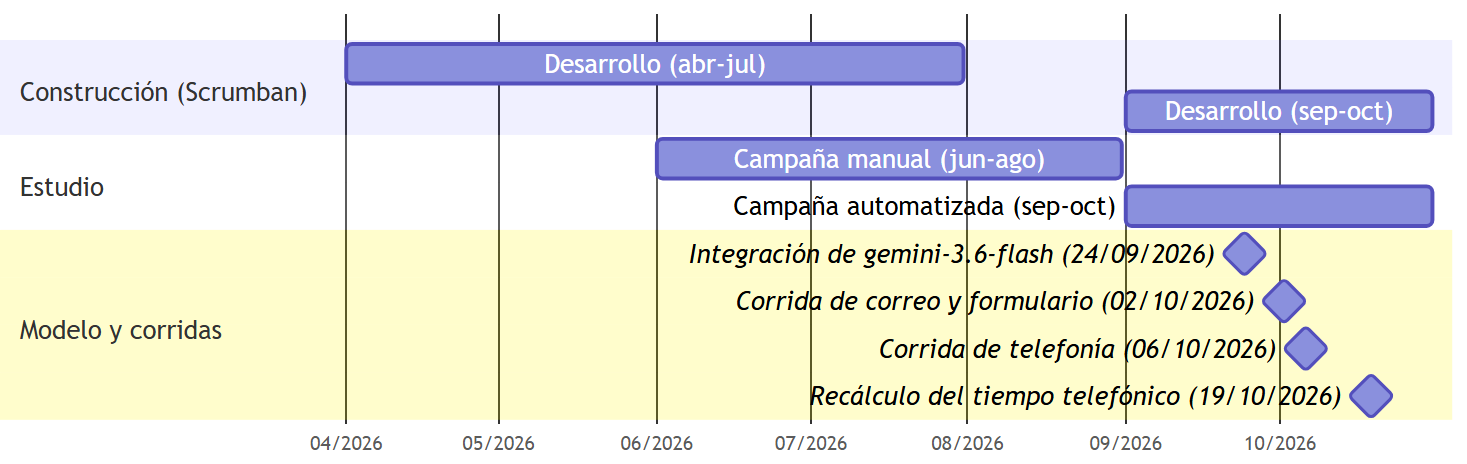
\includegraphics[width=\textwidth,height=0.28\textheight,keepaspectratio]{cronograma}
\caption{Cronograma de la construcción, las campañas y la versión del modelo (barras con precisión de mes; hitos, de día). Fuente: historial del repositorio y confirmación de los autores (9-10-2026).}
\label{fig:cronograma}
\end{figure}

\section{Repositorio de código fuente}\label{sec:anexo-repositorio}

El código fuente del módulo Python, los scripts de migración de la base de datos PostgreSQL gestionados mediante Alembic, los archivos de configuración del despliegue en contenedores Docker y los flujos de integración continua sobre GitHub Actions se encuentran disponibles en el repositorio público del proyecto \parencite{Gomez2026_repositorio}, accesible en \url{https://github.com/lucaGomezB/Automatizacion-de-Mesa-de-Ayuda-N8N}. El commit de referencia para la versión entregada al jurado se identifica con el tag anotado \texttt{v1.2.1}, creado sobre el commit definitivo del repositorio.

El hash completo de ese commit es \texttt{\small 509ffff105c21fed0c07cbf9a46245ba6c53e0e1}, que constituye la referencia verificable de la versión corregida.

La estructura del repositorio separa el módulo de procesamiento (\texttt{App/Backend/}, con la aplicación FastAPI, las migraciones Alembic y las pruebas), la interfaz de usuario (\texttt{App/Frontend/}, React con TypeScript), la definición del flujo de orquestación (\texttt{n8n/workflow.json}), los artefactos de evaluación (\texttt{evaluation/}), el corpus pseudonimizado (\texttt{data/}), los scripts auxiliares (\texttt{scripts/}) y la documentación (\texttt{docs/}), junto con las especificaciones de los changes (\texttt{openspec/}) y los archivos de orquestación local \texttt{docker-compose.yml} y \texttt{Makefile}. El archivo \texttt{README.md} describe esta organización y reúne las instrucciones detalladas para el despliegue local en menos de 15 minutos, por lo que constituye el punto de entrada al código fuente disponible en el repositorio público \parencite{Gomez2026_repositorio}.

\section{Esquema de base de datos}\label{sec:anexo-esquema-bd}

El esquema completo de la base de datos PostgreSQL se documenta mediante scripts SQL versionados que definen las siete entidades descritas en la Tabla~\ref{tab:entidades} de la \autoref{sec:arquitectura}, las restricciones de integridad referencial (claves foráneas con eliminación en cascada condicional), los índices secundarios sobre los atributos de búsqueda frecuente (fecha de creación, sector responsable y estado actual del ticket), y la generación de los identificadores de incidente. Las migraciones incrementales se gestionan mediante Alembic, lo que permite reproducir el estado de la base en cualquier punto histórico del desarrollo y revertir cambios cuando resulte necesario.

La migración inicial incluye la creación de las tablas de catálogo (\texttt{sector}, \texttt{estado}, \texttt{canal\_origen}) con sus valores semilla, garantizando que un despliegue nuevo del sistema comience con los datos de referencia correctos. Las migraciones subsiguientes documentan la evolución del esquema durante las etapas de desarrollo descritas en la \autoref{sec:marco-metodologico}.

El diagrama entidad-relación de las siete entidades se incluye como Figura~\ref{fig:er_modelo_datos} de la \autoref{sec:arquitectura}; su fuente Mermaid versionada reside en \texttt{docs/diagrams/er\_modelo\_datos.md}.

\section{Especificación OpenAPI de la interfaz REST}\label{sec:anexo-openapi}

La especificación completa de la interfaz REST se genera automáticamente mediante FastAPI conforme a la versión~3.1 de la especificación OpenAPI \parencite{Tiangolo2024_fastapi}. El documento resultante describe los puntos de entrada listados en la Tabla~\ref{tab:api} de la \autoref{sec:arquitectura}, los esquemas de los cuerpos de solicitud y respuesta validados mediante Pydantic~v2, los códigos de estado posibles para cada método HTTP, y ejemplos representativos para cada caso de uso.

La interfaz se encuentra disponible adicionalmente en formato interactivo a través del componente Swagger UI integrado en el servidor, accesible bajo la ruta \texttt{/docs} durante la ejecución, y en formato estático como archivo \texttt{openapi.json} en el directorio \texttt{docs/} del repositorio. La sincronización entre el código y la especificación estática se verifica automáticamente en el pipeline de integración continua.

La especificación OpenAPI vigente describe 33 puntos de entrada que exponen 41 métodos HTTP y 44 esquemas de datos, agrupados por recurso: autenticación, catálogos, clasificaciones, incidentes, directorio, estadísticas, telefonía, control de costo y salud.

A título ilustrativo, los 44 esquemas de datos comprenden las estructuras de los catálogos, las entidades de dominio y los objetos de respuesta de cada recurso. El esquema \texttt{IncidenteRead}, por ejemplo, expone el identificador del ticket, la descripción pseudonimizada, la prioridad, el sector y los sectores adicionales, el estado, el canal de origen, el reportante, las marcas temporales de ingreso y persistencia, y los indicadores de latencia end-to-end y de latencia anómala, con sus tipos y campos de solo lectura. El detalle exhaustivo de atributos, tipos y ejemplos reside en \texttt{docs/openapi.json}.

\section{Configuración del flujo N8N}\label{sec:anexo-flujo-n8n}

La exportación del flujo de orquestación en formato JSON incluye la totalidad de los 32 nodos configurados, sus parámetros operativos, las credenciales referenciadas mediante identificadores opacos sin exposición de valores, y los conectores entre nodos. El archivo \texttt{n8n/workflow.json} contiene esta exportación. La importación de este artefacto en una instancia limpia de N8N~2.11.2 reproduce íntegramente el comportamiento operativo del sistema, sujeta únicamente a la provisión de las credenciales correspondientes a los servicios externos integrados (servidor IMAP de correo, cuenta Twilio y clave de API de Gemini) mediante el sistema de credenciales nativo de la plataforma.

La Figura~\ref{fig:anexo_flujo_n8n} presenta una reconstrucción esquemática del flujo, derivada de la exportación JSON y agrupada por etapa funcional. Los 29 nodos operativos (más 3 notas adhesivas, 32 nodos en total) se organizan en siete etapas: entrada (triggers), con la recepción de correo por IMAP y los disparadores de telefonía, formulario web y notificación de clasificación; validación y normalización de la información de entrada, incluida la marca de canal y el sellado de ingreso; envío al backend, con la autenticación del operador y la solicitud POST del incidente; ruteo por canal de origen; revisión humana, con la notificación al operador designado y las respuestas de handoff; respuesta y auditoría del ticket; y aviso post-revisión. La parametrización completa de cada nodo reside en \texttt{n8n/workflow.json}.

\begin{figure}[htbp]
\centering
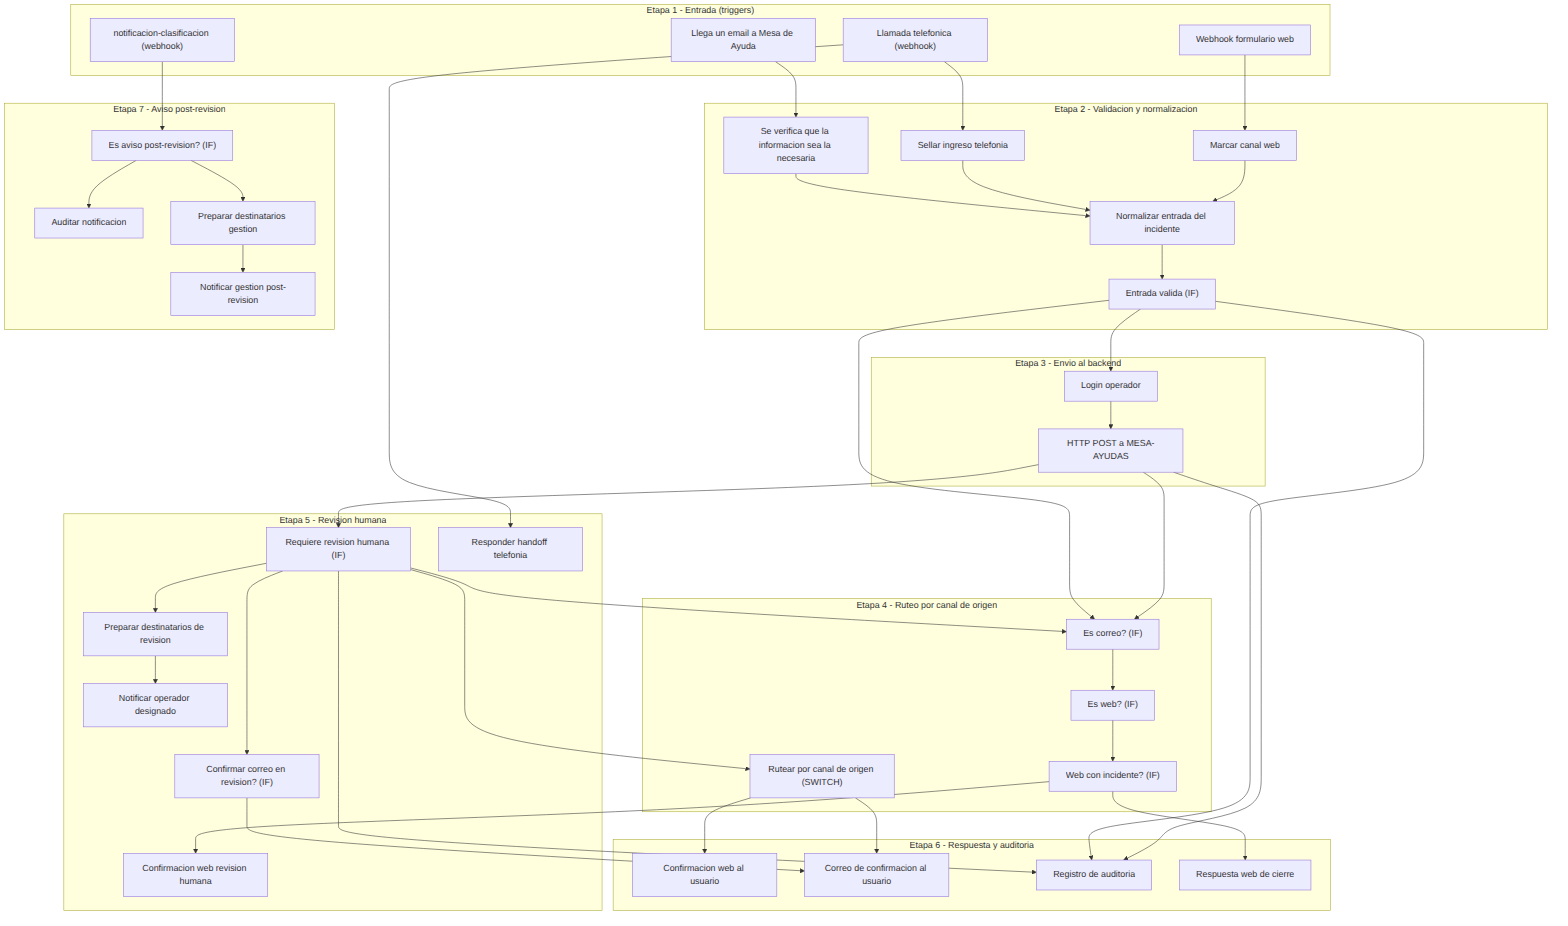
\includegraphics[width=\textwidth]{flujo_n8n}
\caption[Reconstrucción esquemática del flujo de orquestación N8N]{Reconstrucción esquemática del flujo de orquestación N8N: no es una captura de la interfaz; los 29 nodos operativos se agrupan por etapa funcional.}
\label{fig:anexo_flujo_n8n}
\end{figure}

\section{Corpus de validación}\label{sec:anexo-corpus}

El corpus de 200 incidentes utilizado para la validación experimental reside en el repositorio en formato JSON, en su forma pseudonimizada y versionada, bajo la ruta \texttt{data/corpus\_evaluacion\_pseudonimizado.json}. Cada caso incluye el identificador anónimo, la descripción cruda pseudonimizada, el canal de origen, el sector asignado por consenso humano, los sectores adicionales de verdad y el tiempo de registro medido en cada flujo. La categoría predicha por el clasificador y la confianza asociada no forman parte del corpus: se conservan en \texttt{evaluation/predicciones.json}, generado por el framework de evaluación. Se incluyen además las planillas de cronometraje del flujo manual y los registros automáticos generados por el flujo automatizado.

Cada uno de los 200 casos del corpus se compone de siete campos: \texttt{id} (identificador anónimo, por ejemplo \texttt{R001}), \texttt{descripcion} (texto pseudonimizado, con los identificadores personales reemplazados por etiquetas genéricas como \texttt{[EMAIL]}, \texttt{[TELEFONO]}, \texttt{[HOST]} y \texttt{[PERSONA]}), \texttt{canal\_origen} (correo electrónico, formulario web o llamada telefónica), \texttt{sector\_asignado} (sector principal de verdad, exactamente uno de los cinco sectores canónicos), \texttt{sectores\_adicionales} (sectores de verdad complementarios, sin repetir el asignado), \texttt{tiempo\_manual\_s} (tiempo de clasificación manual, en segundos) y \texttt{tiempo\_automatizado\_s} (tiempo del sistema automatizado, en segundos). El corpus completo reside en \texttt{data/corpus\_evaluacion\_pseudonimizado.json} y las predicciones del clasificador en \texttt{evaluation/predicciones.json}.

Por razones de privacidad y en cumplimiento de la Ley~25.326 \parencite{Ley25326_2000}, las descripciones textuales han sido pseudonimizadas previamente a su inclusión en el repositorio público, reemplazando nombres propios, direcciones de correo y otros identificadores personales por etiquetas genéricas.

\section{Documentación operativa}\label{sec:anexo-documentacion-operativa}

La documentación operativa del sistema, que reúne los procedimientos de despliegue, configuración, respaldo y restauración, monitoreo y respuesta ante incidentes operativos, se versiona en el repositorio junto con el código fuente; el runbook operativo reside en \texttt{docs/operational-guide.md}.

\section{Especificación del prompt de Gemini 3.6 Flash}
\label{anexo:H}

Este anexo documenta la especificación del prompt enviado al modelo \texttt{gemini-3.6-flash} (Gemini~3.6 Flash en el texto) y los parámetros de configuración de la inferencia. El prompt se mantiene en el repositorio bajo \texttt{docs/prompt\_gemini.txt} y es único para los tres canales de entrada.

\subsection{Estructura y contenido del prompt}\label{subsec:anexo-estructura-prompt}

El prompt sigue una estructura fija en español organizada en cinco componentes funcionales y un conjunto de reglas de desambiguación:

\begin{enumerate}
  \item \textbf{Instrucción de rol}: define que el modelo actúa como agente especializado en clasificación de incidentes técnicos en español rioplatense, lo que ancla el comportamiento en el dominio y el dialecto del estudio.
  \item \textbf{Definición de categorías}: presenta los cinco sectores canónicos con sus \emph{strings} exactos (sensibles a mayúsculas y sin tildes), un ámbito descriptivo por sector y un ejemplo representativo extraído del dominio real por cada uno.
  \item \textbf{Formato de respuesta}: solicita un JSON válido con exactamente dos campos, \texttt{categoría} (uno de los cinco valores canónicos) y \texttt{confianza} (número entre 0,0 y 1,0), sin texto adicional, comentarios ni explicaciones.
  \item \textbf{Lógica de decisión}: indica analizar la descripción y asignar una categoría única entre las cinco opciones; ante elementos de múltiples categorías, elegir la dominante.
  \item \textbf{Validación sintáctica}: exige validar la corrección sintáctica del JSON antes de devolverlo y reducir la confianza cuando no sea posible clasificar con seguridad.
  \item \textbf{Reglas de desambiguación de frontera}: las acciones sobre aplicaciones o sistemas operativos (acceder, iniciar sesión, abrir una aplicación) se orientan a \texttt{Soporte Tecnico Software}; los dispositivos físicos y su digitalización (escáner, impresora, periférico, error de digitalización) a \texttt{Soporte Tecnico Hardware}; y la infraestructura y los servicios de plataforma (servidor, red, SMTP, VM) a \texttt{Sistemas}. Estas reglas corrigen casos de frontera medidos sobre el corpus.
\end{enumerate}

\subsection{Parámetros de configuración}\label{subsec:anexo-parametros-config}

La invocación del modelo se realiza mediante el SDK \texttt{google-genai} (\texttt{>=2.20.0}), con los hiperparámetros que resume la Tabla~\ref{tab:anexo_gemini_params}, que corresponden a la configuración adoptada para el despliegue y no al resultado de una calibración documentada frente a valores alternativos (\autoref{subsec:capa-procesamiento}).

\begin{table}[htbp]
\small
\centering
\caption{Parámetros de configuración de la inferencia con \texttt{gemini-3.6-flash}.}
\label{tab:anexo_gemini_params}
\begin{tabular}{@{}>{\raggedright\arraybackslash}p{3.0cm} >{\raggedright\arraybackslash}p{2.6cm} >{\raggedright\arraybackslash}p{8.4cm}@{}}
\toprule
Parámetro & Valor & Justificación \\
\midrule
\texttt{temperature} & 0,3 & Valor bajo que reduce la variabilidad de la generación y mejora la consistencia en tareas de clasificación determinística. \\
\texttt{top\_p} & 0,9 & \emph{Nucleus sampling} que admite variantes léxicas válidas en español rioplatense sin sacrificar coherencia. \\
\texttt{max\_tokens} & 100 & Límite suficiente para la respuesta JSON, con margen ante variaciones y sin truncamiento. \\
\texttt{candidate\_count} & 1 & Respuesta única sin remuestreo, que acota la latencia del procesamiento en tiempo real. \\
\texttt{safety\_settings} & Parcialmente desactivados & Desactiva filtros que podrían rechazar descripciones legítimas de incidentes, manteniendo los filtros contra contenido verdaderamente tóxico. \\
\texttt{timeout} & 30 segundos por intento; 60 segundos en total & Límite de latencia por intento del backend al modelo (hasta dos reintentos ante fallas transitorias, dentro de un presupuesto total de 60 segundos por clasificación; no son reintentos de N8N al backend); al agotarse, el clasificador devuelve confianza 0,0 y marca el caso para revisión humana. \\
Umbral de revisión humana & 0,70 & Confianza mínima de una respuesta del modelo para no marcarla para revisión; no se aplica a la etapa determinística (\autoref{subsec:subsistema-clasificacion}). \\
SDK & \texttt{google-genai} \texttt{>=2.20.0} & Versión vigente al momento del estudio, documentada para reproducibilidad. \\
\bottomrule
\end{tabular}
{\footnotesize\textit{Fuente:} elaboración propia a partir de la documentación del SDK \texttt{google-genai}.\par}
\end{table}

\subsection{Validación de la respuesta}\label{subsec:anexo-validacion-respuesta}

Antes de aceptar la respuesta del modelo, el módulo de clasificación valida que el texto sea JSON parseable, que contenga exactamente las claves \texttt{categoría} y \texttt{confianza}, que la categoría sea uno de los cinco valores canónicos y que la confianza sea un número en el intervalo \([0{,}0, 1{,}0]\). Si cualquiera de estas condiciones falla, se registra la excepción, se asigna confianza 0,0, se marca el incidente para revisión humana y no se propagan estados inconsistentes a la base de datos. Este procedimiento garantiza la confiabilidad operativa frente a errores de formato o alucinaciones del modelo. El Listado~\ref{lst:validar-gemini} resume la rutina de validación.

\begin{lstlisting}[caption={Validación de la respuesta de Gemini (resumen).},label={lst:validar-gemini}]
def validar_respuesta_gemini(response_text: str) -> tuple[bool, dict]:
    try:
        data = json.loads(response_text)
    except json.JSONDecodeError as e:
        return False, {"error": f"JSON invalido: {e}"}
    if "categoria" not in data:
        return False, {"error": "Falta campo 'categoria'"}
    if data["categoria"] not in SECTORES_CANONICOS:
        return False, {"error": f"Categoria invalida: {data['categoria']}"}
    if "confianza" not in data:
        return False, {"error": "Falta campo 'confianza'"}
    if not isinstance(data["confianza"], (int, float)) \
            or not (0.0 <= data["confianza"] <= 1.0):
        return False, {"error": f"Confianza invalida: {data['confianza']}"}
    return True, data
\end{lstlisting}

\subsection{Iteración y mejora del prompt}\label{subsec:anexo-iteracion-prompt}

El prompt de la versión evaluada se ajustó de forma iterativa a partir de errores observados en el corpus de validación; no se dispuso de un corpus independiente de preproducción. Las versiones históricas del prompt se conservan en el historial de versiones del repositorio (archivo \texttt{docs/prompt\_gemini.txt}) para auditoría y eventual reversión.

\subsection{Recomendaciones para futuras iteraciones}\label{subsec:anexo-recomendaciones-prompt}

Ante una degradación de las métricas por cambios en el modelo, se recomienda profundizar los ejemplos por clase (de dos a cuatro o cinco), agregar contraejemplos de incidentes limítrofes, especificar umbrales de confianza explícitos, incluir un diccionario de términos clave por categoría y, una vez acumulado un corpus del orden de 5.000 casos etiquetados (referencia indicativa de orden de magnitud, no derivada del corpus actual ni de un cálculo de potencia estadística), migrar a un modelo ajustado específicamente al dominio.

\section{Trazabilidad de las correcciones del dictamen}\label{sec:anexo-trazabilidad}

El registro de correcciones derivado del dictamen evaluador se conserva como artefacto versionado en el repositorio, bajo la ruta \texttt{docs/Tesis/Correcciones/dictamen-correcciones.md}. El documento compila, de forma acumulativa, cada corrección aplicada al manuscrito y las decisiones adoptadas sobre las observaciones que no admitían una resolución inmediata (por ejemplo, la convención estadística del estadístico \emph{W}, la reformulación de la hipótesis principal y el tratamiento de los reintentos como limitación conocida). Se incluye aquí como ejemplo de trazabilidad: cada entrada del registro vincula una observación del dictamen con el archivo y la línea corregidos, de modo que la correspondencia entre la revisión solicitada y la revisión efectuada resulte auditable de extremo a extremo.

El dictamen que motiva las correcciones vigentes es el emitido el 22 de octubre de 2026 sobre la versión de trabajo v10, publicada como \texttt{v1.1.0} y aplicable por igual a \texttt{v1.1.1}. Sus cinco observaciones de fondo (A1 a A5) y sus correcciones de consistencia (B4 a B16) se atendieron mediante changes del repositorio; la \autoref{tab:anexo-trazabilidad} indica, para cada una, el change responsable y las secciones de la tesis donde se la atendió. Cuando una recomendación se dividió en partes, figuran los changes que las atendieron.

\begin{table}[htbp]
\small
\centering
\caption{Recomendaciones del dictamen del 22 de octubre de 2026, change responsable y secciones donde se atendieron.}
\label{tab:anexo-trazabilidad}
\setlength{\tabcolsep}{4pt}
\begin{tabular}{@{}>{\raggedright\arraybackslash}p{1.0cm} >{\raggedright\arraybackslash}p{3.3cm} >{\raggedright\arraybackslash}p{10.6cm}@{}}
\toprule
Rec. & Change & Secciones de la tesis \\
\midrule
A1 & \texttt{c-130} & \autoref{subsec:human-in-the-loop}, \autoref{subsec:subsistema-clasificacion}, \autoref{subsec:construccion-flujo-n8n}, \autoref{subsec:reduccion-intervencion} \\
A2 & \texttt{c-131} & \autoref{subsec:calibracion}, \autoref{tab:bandas}, \autoref{tab:exactitud-etapa-canal}, \autoref{subsec:interpretacion-resultados} \\
A3 & \texttt{c-132} & \autoref{subsec:balance-neto}, \autoref{subsec:implicancias-practicas} \\
A4 & \texttt{c-139}, \texttt{c-138} & \autoref{subsec:nlp-llm}, \autoref{subsec:trabajos-academicos}, \autoref{subsec:calibracion-cascadas}, \autoref{subsec:clasificador-supervisado} \\
A5 & \texttt{c-130}, \texttt{c-144}, \texttt{c-142} & \autoref{subsec:subsistema-clasificacion}, \autoref{subsec:conexion-scrumban}, \autoref{subsec:interpretacion-resultados}, \autoref{subsec:anexo-iteracion-prompt}; \autoref{subsec:sensibilidad-ajustes}, \autoref{subsec:limitaciones-estudio} \\
B4 & \texttt{c-133} & \autoref{tab:cumplimiento-objetivos}, \autoref{subsec:cumplimiento-objetivos} \\
B5 & \texttt{c-133} & \autoref{subsec:hipotesis-trabajo} \\
B6 & \texttt{c-133} & \autoref{subsec:metricas-instrumentos}, \autoref{tab:metricas} \\
B7 & \texttt{c-134}, \texttt{c-131} & \autoref{tab:tiempos-canal}; \autoref{tab:exactitud-etapa-canal} \\
B8 & \texttt{c-131} & \autoref{subsec:metricas-instrumentos}, \autoref{tab:exactitud-etapa-canal} \\
B9 & \texttt{c-135} & \autoref{subsec:gestion-scrumban}, \autoref{subsec:conexion-scrumban}, \autoref{fig:cronograma}, \autoref{subsec:limitaciones-estudio} \\
B10 & \texttt{c-135} & \autoref{sec:resultados}, \autoref{tab:comparativa}, \autoref{tab:trabajos-academicos} \\
B11 & \texttt{c-136} & \autoref{sec:recomendaciones}, \autoref{subsec:calibracion-gate}, \autoref{subsec:medicion-intervencion}, \autoref{subsec:aprendizaje-activo} \\
B12 & \texttt{c-134} & \autoref{subsec:analisis-estadistico}, \autoref{subsec:poblacion-muestra-corpus} \\
B13 & \texttt{c-135}, \texttt{c-134} & \autoref{subsec:cumplimiento-objetivos}; \autoref{subsec:diseno-experimental}, \autoref{subsec:consentimiento-derechos} \\
B14 & \texttt{c-137} & Todo el documento (revisión ortotipográfica) \\
B15 & \texttt{c-139} & \autoref{subsec:cumplimiento}, \autoref{subsec:analisis-estadistico} \\
B16 & \texttt{c-139}, \texttt{c-141} & \autoref{sec:anexo-repositorio} y Referencias bibliográficas \\
\bottomrule
\end{tabular}
\par\smallskip
{\footnotesize\textit{Fuente:} elaboración propia a partir de \texttt{docs/Tesis/Correcciones/dictamen-correcciones.md}.\par}
\end{table}

La trazabilidad interna de dos decisiones que el cuerpo del Capítulo~6 presenta en lenguaje llano se conserva aquí: el retiro de la rama de clasificación telefónica por agente LLM basada en LangChain y el traslado de la superficie de costo al backend corresponden al change \texttt{c-72}. El detalle de ambas decisiones figura en \texttt{docs/Tesis/Correcciones/dictamen-correcciones.md}.

\newpage

}
\end{appendices}

\end{document}
